% Type of document (article, report, book)
% scrreprt is from koma-script
\documentclass[a4paper, top=2cm, bottom=2cm, left=2.5cm, right=2.5cm, chapterprefix=true, numbers=noenddot]{scrreprt}

%%% PACKAGES %%%

\RedeclareSectionCommand[beforeskip=60pt, afterskip=40pt, font=\fontsize{25}{50}\selectfont\bfseries]{chapter}

% Define chapter and section title format
% add unicode support
\usepackage[utf8]{inputenc}

% Use Helvetica as font
\usepackage[scaled]{helvet}
\renewcommand\familydefault{\sfdefault}
\usepackage[T1]{fontenc}

\usepackage{multirow}

% Better tables
\usepackage{tabularx}

% Better enumerisation env
\usepackage{enumitem}

% Use graphics
\usepackage{graphicx}

% Use date and time
\usepackage{datetime}

% Have subfigures and captions
\usepackage{subcaption}

% Be able to include PDFs in the file
\usepackage{pdfpages}

% Have custom abstract heading
\usepackage{abstract}

% Need a list of equation
\usepackage{tocloft}
\usepackage{ragged2e}

% Better equation environment
\usepackage{amsmath}

% Symbols for most SI units
\usepackage{siunitx}

\usepackage{csquotes}

% Change page rotation
\usepackage{pdflscape}

% Symbols like checkmark
\usepackage{amssymb}
\usepackage{pifont}

\usepackage[absolute]{textpos}

% Glossary, hyperref, babel, polyglossia, inputenc, fontenc must be loaded before this package if they are used
%\usepackage{glossaries}
% Redefine the quote charachter as we are using ngerman
%\GlsSetQuote{+}
% Define the usage of an acronym, Abbreviation (Abbr.), next usage: The Abbr. of ...
%\setacronymstyle{long-short}

% Bibliography & citing
\usepackage[
	backend=biber,
	style=apa,
	bibstyle=apa,
	citestyle=apa,
	]{biblatex}
\addbibresource{references.bib}

% Clickable Links to Websites and chapters
% From the documentation: "Make sure it comeslastof your loaded packages, to give it a fighting chance of not beingover-written, since its job is to redefine many LATEX commands"
\usepackage{hyperref}

%%% COMMAND REBINDINGS %%%
\newcommand{\tabitem}{~~\llap{\textbullet}~~}
\newcommand{\xmark}{\ding{55}}
\newcommand{\notmark}{\textbf{\textasciitilde}}
% Pro/Con item https://tex.stackexchange.com/questions/145198/change-the-bullet-of-each-item#145203
\newcommand\pro{\item[$+$]}
\newcommand\con{\item[$-$]}

% Define list of equations - Thanks to Charles Clayton: https://tex.stackexchange.com/a/354096
\newcommand{\listequationsname}{\huge{List of Formulas}}
\newlistof{myequations}{equ}{\listequationsname}
\newcommand{\myequations}[1]{
	\addcontentsline{equ}{myequations}{\protect\numberline{\theequation}#1}
}
\setlength{\cftmyequationsnumwidth}{2.3em}
\setlength{\cftmyequationsindent}{1.5em}

% Usage {equation}{caption}{label}
% \indexequation{b = \frac{\pi}{\SI{180}{\degree}}\cdot\beta\cdot 6378.137}{Bogenlänge $b$ des Winkels $\beta$ mit Radius 6378.137m (Distanz zum Erdmittelpunkt am Äquator)}{Bogenlaenge}
\newcommand{\indexequation}[3]{
	\begin{align} \label{#3} \ensuremath{\boxed{#1}} \end{align}
	\myequations{#3} \centering \small \textit{#2} \normalsize \justify }

% Todolist - credit to https://tex.stackexchange.com/questions/247681/how-to-create-checkbox-todo-list
\newlist{todolist}{itemize}{1}
\setlist[todolist]{label=$\square$}

% Nested Enumeratelist credit to https://tex.stackexchange.com/a/54676
\newlist{legal}{enumerate}{10}
\setlist[legal]{label*=\arabic*.}

%%% PATH DEFINITIONS %%%
% Define the path were images are found
\graphicspath{{./img/}{./appendix/}}

%%% GLOSSARY ENTRIES %%%
%\makeglossaries
% \newacronym{RFID}{RFID}{Radio-Frequency Identification}
% \newglossaryentry{HF}{name={HF},description={High Frequency, RFID Tags im Frequenzbereich von 3-30MHz}}

\usepackage{fancyhdr}
\usepackage[top=2.5cm, bottom=2.5cm, left=3.0cm, right=2.5cm]{geometry}

% Clear all header and footer fields
\fancyhf{}

% Header settings
\fancyhead[R]{\leftmark} % Display chapter or section name on the right side of header
\setlength{\headsep}{0.5cm} % Add margin for header text

% Footer settings
\fancyfoot[C]{\thepage\hspace{1.5cm}} % Display page number in the center of footer with added space
\setlength{\footskip}{1.25cm} % Add margin for footer text

% Set the height of the header
\setlength{\headheight}{14.5pt}

% Apply the custom style to the "plain" page style
\fancypagestyle{plain}{%
    \fancyhf{} % Clear all header and footer fields
    \fancyfoot[C]{\thepage\hspace{1.5cm}} % Display page number in the center of footer with added space
    \renewcommand{\headrulewidth}{0pt} % Remove header rule
}

% Apply the custom style to all other page styles
\pagestyle{fancy}


%%% TODO Notes %%%
\usepackage{todonotes}

%%% Code %%%
\usepackage{listings}
\lstset{
  basicstyle=\ttfamily,
  columns=fullflexible,
  frame=single,
  breaklines=true,
  postbreak=\mbox{\textcolor{red}{$\hookrightarrow$}\space},
}

%%% No styling for toc etc. %%%
\addtocontents{toc}{\protect\thispagestyle{empty}}
\addtocontents{lof}{\protect\thispagestyle{empty}}
\addtocontents{lot}{\protect\thispagestyle{empty}}

%%% Tables %%%
\usepackage{booktabs}

%%% Image Placement %%%
\usepackage{floatrow}
\floatsetup[figure]{capposition=bottom}

%%% DOCUMENT %%%

\begin{document}

\begin{titlepage}
	\begin{center}
		\null
		\today
	\end{center}
\end{titlepage}

\newpage

\pagenumbering{gobble}

\raggedright

\textbf{\Large Bachelor Thesis at Lucerne University of Applied Sciences and Arts}\\[0.1cm]
\textbf{\Large School of Computer Science and Information Technology}\\[0.5cm]

\rule{\linewidth}{0.5mm}\\[0.4cm]
{\huge \bfseries Automated Image Quality Assessment in Teledermatology}\\[0.2cm]
\rule{\linewidth}{0.5mm}\\[0.5cm]

\textbf{Name of Student:} Nyungmartsang Choekyel\\
\textbf{Degree Program:} B.Sc. in Artificial Intelligence and Machine Learning\\
\textbf{Year of Graduation:} 2024\\[0.8cm]

\textbf{Main Advisor:} Dr. Amruthalingam Ludovic\\
\textbf{External Expert:} xxx\\
\textbf{Industry partner/provider:} ABIZ, University Hospital of Basel and derma2go\\[0.8cm]

\textbf{Code / Thesis Classification:}\\
\begin{itemize}
	\item[$\checkmark$] Public (Standard)
	\item[$\square$] Private
\end{itemize}
\vspace{0.4cm}

\textbf{Declaration}\\[0.5cm]
I hereby declare that I have completed this thesis alone and without any unauthorized or external help. I further declare that all the sources, references, literature and any other associated resources have been correctly and appropriately cited and referenced. The confidentiality of the project provider (industry partner) as well as the intellectual property rights of the Lucerne University of Applied Sciences and Arts have been fully and entirely respected in completion of this thesis.\\[0.8cm]

\begin{tabularx}{\textwidth}{@{}lX}
	&\\
	Rotkreuz, \today &  \\
	\cline{2-2}
	&\\[0.75cm]
\end{tabularx}

\textbf{Submission of the Thesis to the Portfolio Database:}\\[0.5cm]
\textbf{Confirmation by the student}\\[0.2cm]
I hereby confirm that this bachelor thesis has been correctly uploaded to the Portfolio Database in line with the code of practice of the University. I rescind all responsibility and authorization after upload so that no changes or amendments to the document may be undertaken.\\[0.8cm]

\begin{tabularx}{\textwidth}{@{}lX}
	&\\
	Rotkreuz, \today &  \\
	\cline{2-2}
	&\\[0.75cm]
\end{tabularx}

\newpage

\pagenumbering{gobble}

\chapter*{Expression of Thanks and Gratitude}

Expression of thanks and gratitude here...

\vfill

\emph{Intellectual property of the degree programs of the Lucerne
University of Applied Sciences and Arts, FH Zentralschweiz, in
accordance with Student Regulations:
\href{https://srl.lu.ch/app/de/texts_of_law/521/versions/4065}{Studienordnung}}




\pagenumbering{Roman}

\chapter*{Abstract}
Text \par
\vspace{\baselineskip}
\noindent
Text \par
\vspace{\baselineskip}
\noindent
Text
\clearpage

\pagestyle{empty}
\tableofcontents \clearpage

\listoffigures 

\listoftables \clearpage

\pagestyle{fancy}

\pagenumbering{arabic}

\chapter{Introduction}
\label{ch:Introduction}
text

\section{Background and Motivation}
\label{sec:BackgroundMotivation}
text \par
\vspace{\baselineskip}
\noindent

\section{Problem Statement}
\label{sec:ProblemStatement}
text \par
\vspace{\baselineskip}
\noindent

\section{Objectives of the Thesis}
\label{sec:Objectives}
text \par
\vspace{\baselineskip}
\noindent

\section{Scope and Limitations}
\label{sec:ScopeLimitations}
text \par
\vspace{\baselineskip}
\noindent

\section{Structure of the Thesis}
\label{sec:Structure}
text \par
\vspace{\baselineskip}
\noindent


\chapter{Literature Review}
\label{ch:LiteratureReview}
Stand der Forschung oder Stand der Praxis/Technik

Bezogen auf die eigenen Zielsetzungen und Fragestellungen soll aufgezeigt werden, wie andere dieses oder ähnliche Probleme gelöst haben. Worauf können Sie aufbauen, was müssen Sie neu angehen? Wodurch unterscheidet sich Ihre Lösung von anderen Lösungen? Für wissenschaftlich orientierte Arbeiten sei hier explizit auf (Balzert, S. 66 ff) verwiesen.

\section{Image Quality Assessment (IQA)}
\label{sec:OverviewTeledermatology}
In this section, the fundamentals of Image Quality Assessment (IQA) will be explored. It will introduce IQA as a field concerned with quantifying the quality of images objectively. The subsection will cover the metrics commonly used in IQA to evaluate image fidelity, clarity, and other quality aspects. Additionally, benchmark datasets utilized in IQA research and the state-of-the-art (SOTA) IQA methods will be discussed. \par
\vspace{\baselineskip}
Image Quality Assessment (IQA) is a vital process aimed at measuring various forms of degradation in images. These degradations include blur, geometric distortions such as shrinking or zooming, and blockiness artifacts resulting from compression standards. IQA primarily focuses on quantifying these degradations to ensure the fidelity and perceptual quality of images. \par
\vspace{\baselineskip}
It's worth noting that while IQA primarily measures degradation, it's closely related to other aspects of image assessment. For instance, Image Aesthetics Assessment evaluates the visual appeal of images as perceived by human eyes, which intersects with IQA. Additionally, Image Fidelity Assessment examines the accuracy of reconstructed images concerning the original view, though the primary focus of IQA remains on measuring degradation. \par

\subsection{Subjective Quality Assessment}
\label{sub:SubjectiveQualityAssessment}
Subjective quality assessment involves human observers evaluating the quality of images based on their visual perception. There are two primary methods employed: Absolute Categorical Rating and Paired Comparison. \par
\begin{itemize}
    \item Absolute Categorical Rating: In this method, human observers view an image and assign a score to its quality based on predefined categories. They evaluate the image independently without any reference image.
    \item Paired Comparison: Here, human observers compare two images: the one under assessment and a reference image. They then assign a quality score based on the perceived difference between the two images. However, Paired Comparison is not feasible in teledermatology due to the absence of a reference image, as the diagnosis of the image is unknown.
\end{itemize}
Subjective quality assessment is known for its accuracy, as it directly involves human perception. However, it is also resource and labor-intensive, requiring human assessors to evaluate each image. Moreover, subjective assessment can be prone to biases introduced by human scorers. \par

\subsection{Objective Quality Assessment}
\label{sub:ObjectiveQualityAssessment}
Objective quality assessment relies on mathematical algorithms rather than human judgment to evaluate image quality. There are three main categories of objective assessment methods: Full-Reference IQA (FR-IQA), Reduced-Reference IQA (RR-IQA), and No-Reference IQA (NR-IQA). \par
\vspace{\baselineskip}
\begin{figure}[ht]
    \centering
    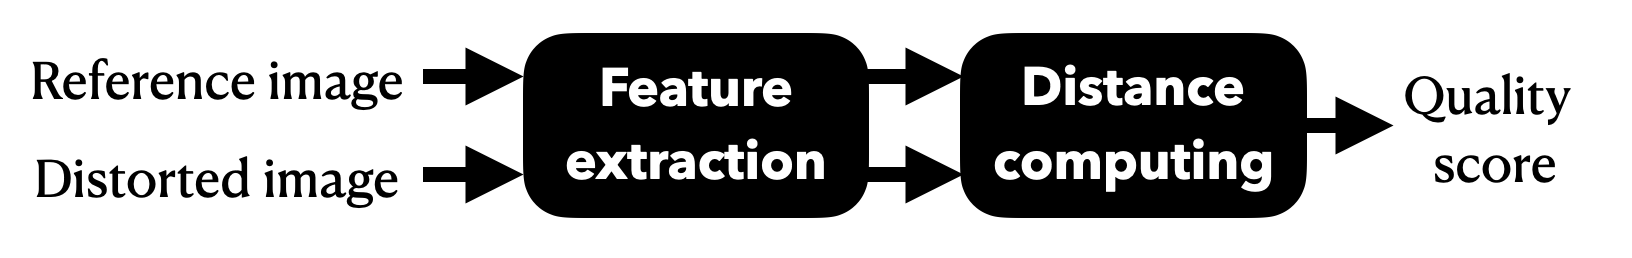
\includegraphics[keepaspectratio,width=15cm]{img/FRIQA.png}
    \caption{Comparison between a distorted image and a reference image to compute quality scores.}
    \label{fig:FRIQA}
\end{figure}
\noindent
\textbf{Full-Reference IQA (FR-IQA):} In FR-IQA \ref{fig:FRIQA}, each distorted image is compared against a reference image. Features are extracted from both images, and their distance is computed to derive a quality score. This method provides a comprehensive assessment but requires a reference image for every distorted image. \par
\vspace{\baselineskip}
\begin{figure}[ht]
    \centering
    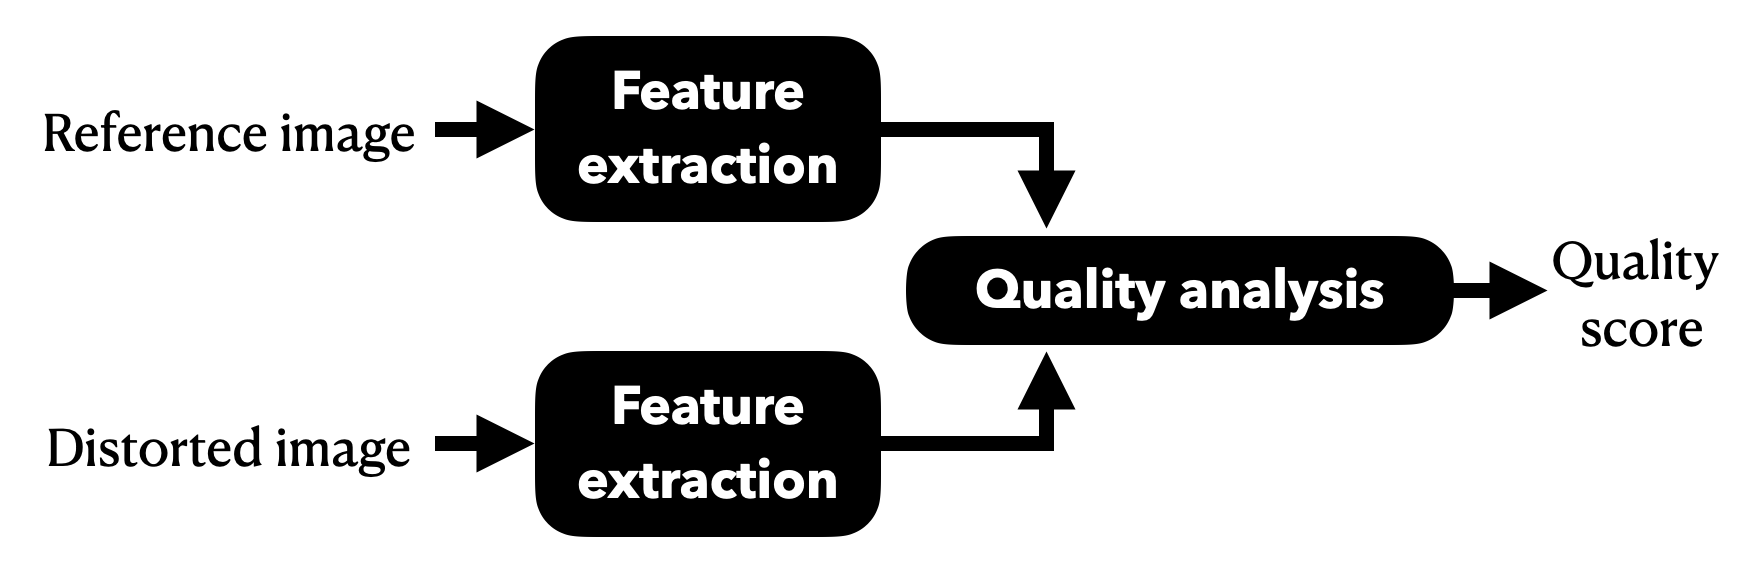
\includegraphics[keepaspectratio,width=15cm]{img/RRIQA.png}
    \caption{Reduced-reference assessment comparing features extracted from distorted and reference images for quality analysis.}
    \label{fig:RRIQA}
\end{figure}
\noindent
\textbf{Reduced-Reference IQA (RR-IQA):} RR-IQA \ref{fig:RRIQA} is similar to FR-IQA but uses a reduced sample of reference images. Features are extracted separately from the distorted image and reference images, and quality is analyzed based on these features. This approach reduces computational complexity but still requires reference information. \par
\vspace{\baselineskip}
Both FR-IQA and RR-IQA utilize two methods to analyze quality:
\begin{itemize}
    \item Spatial-Based Analysis: This method compares images pixel by pixel or region by region, offering straightforward interpretation and efficient computation. However, it may not be robust and is not directly similar to the Human Visual System (HVS).
    \item Transform-Based Analysis: Images are transformed into another domain, such as the frequency domain, mimicking the HVS. While robust, this method is complex, computationally expensive, and less intuitive to interpret.
\end{itemize}
\vspace{\baselineskip}
\begin{figure}[ht]
    \centering
    
\includegraphics[keepaspectratio,width=15cm]{img/NRIQA.png}
    \caption{Quality assessment based solely on features extracted from the distorted image, without a reference image.}
    \label{fig:NRIQA}
\end{figure}
\noindent
\textbf{No-Reference IQA (NR-IQA):} NR-IQA \ref{fig:NRIQA} does not require a reference image; only the distorted image is analyzed. Features are extracted from the distorted image, and quality is predicted based on these features. NR-IQA can focus on single distortions or be designed for general-purpose assessment, making it adaptable for diverse applications. However, it tends to be complex and computationally expensive. \par
\vspace{\baselineskip}
For this study, the focus will be on NR-IQA, particularly in the context of general-purpose quality assessment, aiming to address various distortions encountered in teledermatology images.

\subsection{Common Distortions in IQA}
\label{sub:CommonDistortionsIQA}
Image Quality Assessment (IQA) considers various distortions that affect image quality. \par
The common distortions are \cite{https://arxiv.org/abs/2310.14918}:
\begin{figure}[ht]
    \centering
    \begin{subfigure}[b]{0.24\textwidth}
        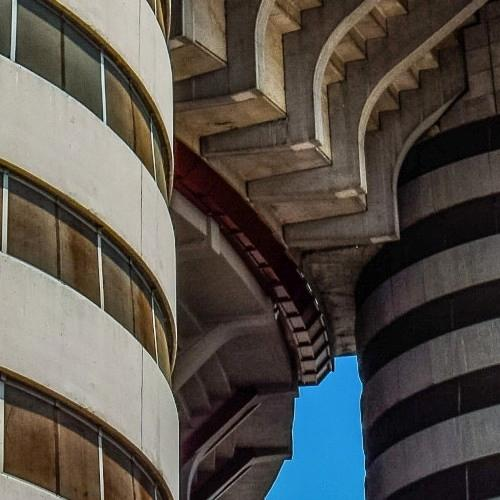
\includegraphics[width=\textwidth]{img/Original.jpg}
        \caption{Original}
    \end{subfigure}
    \hfill
    \begin{subfigure}[b]{0.24\textwidth}
        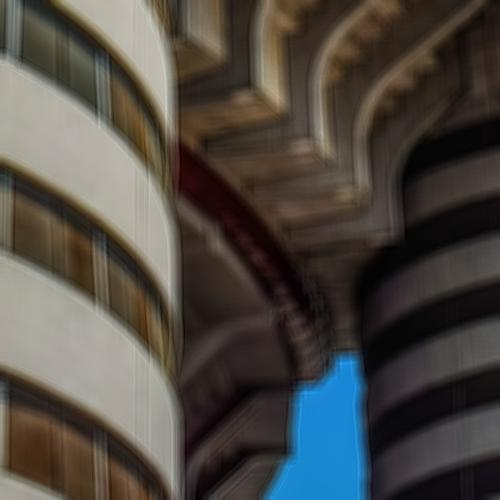
\includegraphics[width=\textwidth]{img/Blur.jpg}
        \caption{Blur}
        \label{fig:blur}
    \end{subfigure}
    \hfill
    \begin{subfigure}[b]{0.24\textwidth}
        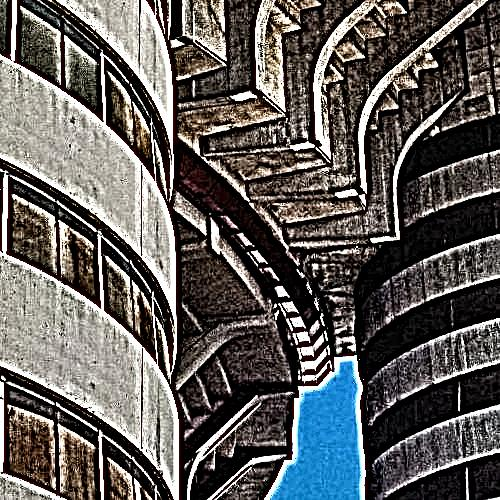
\includegraphics[width=\textwidth]{img/Sharpness.jpg}
        \caption{Sharpness}
        \label{fig:sharpness}
    \end{subfigure}
    \hfill
    \begin{subfigure}[b]{0.24\textwidth}
        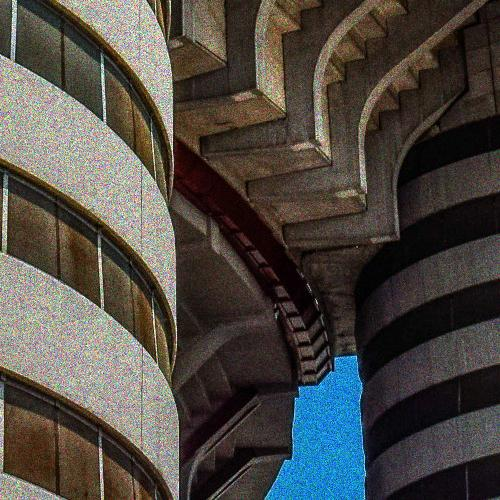
\includegraphics[width=\textwidth]{img/Noise.jpg}
        \caption{Noise}
        \label{fig:noise}
    \end{subfigure} 

    \begin{subfigure}[b]{0.24\textwidth}
        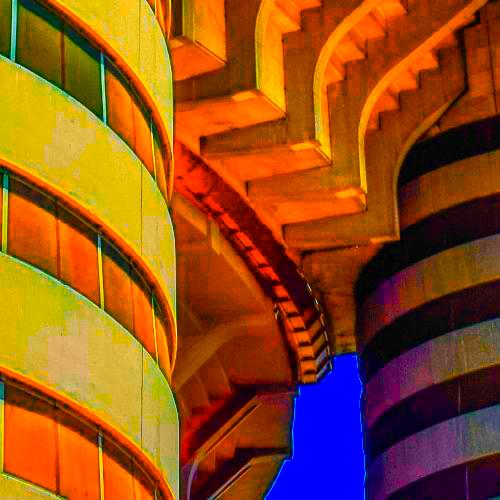
\includegraphics[width=\textwidth]{img/ColorAccuracy.jpg}
        \caption{Color Accuracy}
        \label{fig:color_accuracy}
    \end{subfigure}
    \hfill
    \begin{subfigure}[b]{0.24\textwidth}
        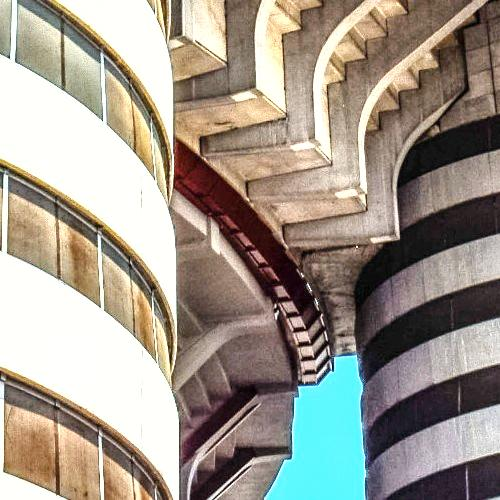
\includegraphics[width=\textwidth]{img/BrightnessContrast.jpg}
        \caption{Brightness \& Contrast}
        \label{fig:brightness_contrast}
    \end{subfigure}
    \hfill
    \begin{subfigure}[b]{0.24\textwidth}
        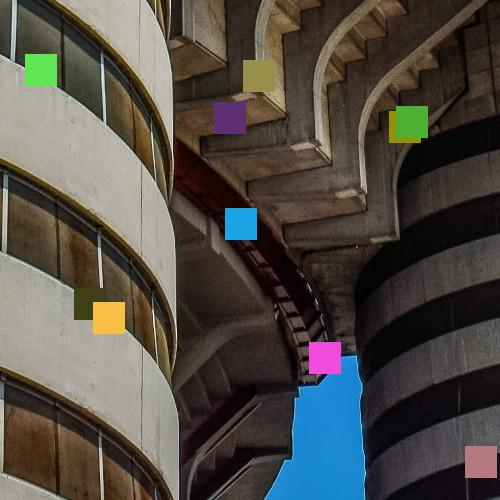
\includegraphics[width=\textwidth]{img/Artifacts.jpg}
        \caption{Artifacts}
        \label{fig:artifacts}
    \end{subfigure}
    \hfill
    \begin{subfigure}[b]{0.24\textwidth}
        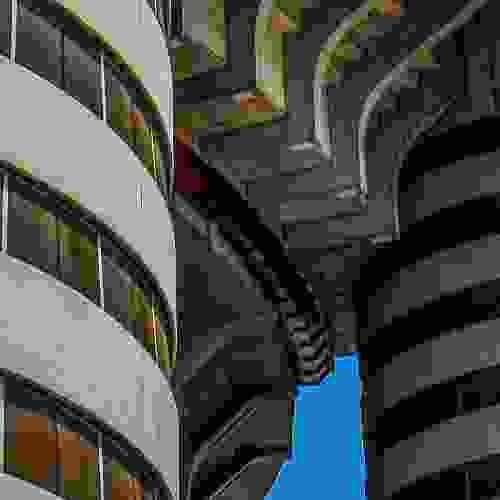
\includegraphics[width=\textwidth]{img/Compression.jpg}
        \caption{Compression}
        \label{fig:compression}
    \end{subfigure}
    \caption{Example images illustrating common distortions used in Image Quality Assessment.}
    \label{fig:distortions}
\end{figure}
\begin{enumerate}
    \item \textbf{Blur}: Blurred images lack sharpness and clarity, often resulting from motion blur, focus issues, or lens imperfections. Example Image: \ref{fig:blur}.
    
    \item \textbf{Sharpness}: Sharpness refers to the clarity and definition of edges and details in an image. Example Image: \ref{fig:sharpness}.
    
    \item \textbf{Noise}: Noise manifests as random variations in brightness or color in an image, typically caused by sensor limitations or high ISO settings. Example Image: \ref{fig:noise}.
    
    \item \textbf{Color Accuracy}: Color accuracy pertains to the faithful reproduction of colors in an image. Distortions in color accuracy can lead to inaccurate or unrealistic color representation. Example Image: \ref{fig:color_accuracy}.
    
    \item \textbf{Brightness \& Contrast}: Brightness refers to the overall lightness or darkness of an image, while contrast relates to the difference in luminance between the lightest and darkest parts. Distortions in brightness and contrast can result in images appearing too dark, too bright, or lacking in tonal range. Example Image: \ref{fig:brightness_contrast}.
    
    \item \textbf{Artifacts}: Artifacts are unwanted visual anomalies introduced during image acquisition or processing, such as compression artifacts, halos, or jagged edges. Example Image: \ref{fig:artifacts}.
    
    \item \textbf{Compression}: Compression distortions occur when an image is compressed to reduce file size, leading to loss of detail and image degradation. Example Image: \ref{fig:compression}.
\end{enumerate}
Each distortion type affects the visual quality and perceptual fidelity of images, influencing the effectiveness of IQA methodologies in assessing image quality. Understanding these distortions is crucial for developing robust quality assessment algorithms and enhancing image fidelity in various applications, including teledermatology.

\subsection{Benchmark Datasets for IQA}
\label{sub:BenchmarkDatasetsIQA}
Benchmark datasets play a crucial role in advancing the field of Image Quality Assessment (IQA) by providing standardized and diverse sets of images with known distortions and corresponding quality annotations. These datasets serve as reference points for evaluating the performance of IQA algorithms and comparing their effectiveness across different distortion types, levels, and image characteristics. \par

By offering a wide range of images spanning various content types, resolutions, and distortion scenarios, benchmark datasets enable researchers to rigorously assess the robustness, accuracy, and generalization capability of IQA methodologies. Furthermore, these datasets facilitate the development of novel algorithms by providing ground-truth quality scores and fostering reproducible research practices. \par

In the following sections, we will explore some prominent benchmark datasets commonly used in the field of IQA, highlighting their key characteristics, contents, and contributions to advancing the state-of-the-art in image quality assessment. \par

\begin{table*}[!t]
    \centering
    \caption{An overview of IQA databases}
    \label{tab:iqa_databases}
    \setlength{\tabcolsep}{0.3em}
    \scalebox{0.57}{
    \renewcommand{\arraystretch}{1.5}
    \begin{tabular}{p{1.8cm} p{2cm} c c c c c c c}
    \toprule
        Category & Database & Year & \#Ref. & \#Dist. & \#Dist. Type & \#Dist. Level & Resolution Type & Ground-truth \\
        \hline
        \multirow{10}{*}{General} 
        & LIVE \cite{LIVE} & 2004 & 30 & 779 & 5 & 5 or 4 & 768 x 512 & DMOS \\
        & TID2008 \cite{TID2008} & 2008 & 25 & 1700 & 17 & 4 & 512 x 384 & MOS \\
        & TID2013 \cite{TID2013} & 2013 & 25 & 3000 & 24 & 5 & 512 x 384 & MOS \\
        & CSIQ \cite{CSIQ} & 2009 & 30 & 866 & 6 & 5 or 4 & 512 x 512 & DMOS \\
        & IVC \cite{IVC} & 2005 & 10 & 54 & 4 & 5 & 512 x 512 & MOS \\
        & MICT \cite{MICT} & 2001 & 14 & 168 & 2 & 6 & 768 x 512 & MOS \\
        & A57 \cite{A57} & 2007 & 3 & 54 & 6 & 3 & 512 x 512 & MOS \\
        & WED \cite{WED} & 2017 & 4744 & 94880 & 4 & 5 & - & - \\
        & KADIS700K \cite{KADIS700K} & - & - & - & - & - & - & - \\
        & KADID \cite{KADID} & - & - & - & - & - & - & - \\
        \hline
        \multirow{3}{*}{Multiple Distortions} 
        & LIVEMD \cite{LIVEMD} & 2012 & 15 & 405 & 2 & - & 1280 x 720 & DMOS \\
        & MDID2013 \cite{MDID2013} & 2013 & 12 & 324 & - & - & 768 x 512 or 1280 x 720 & DMOS \\
        & MDID2016 \cite{MDID2016} & 2016 & 20 & 1600 & - & - & 512 x 384 & MOS \\
        \hline
        \multirow{4}{*}{Screen content} 
        & SIQAD \cite{SIQAD} & 2014 & 20 & 980 & 7 & 7 & 700 x 700 & DMOS \\
        & SCIQ \cite{SCIQ} & 2017 & 40 & 1800 & 9 & 5 & 1280 x 720 & MOS \\
        & CCT \cite{CCT} & 2017 & 72 & 1320 & 2 & 11 & 1280 x 720 to 1920 x 1080 & MOS \\
        & HSNID \cite{HSNID} & 2019 & 20 & 600 & 6 & 5 &  - & MOS \\
        \hline
        \multirow{2}{*}{Authentic} 
        & LIVE Wild \cite{LIVEWild} & 2016 & 0 & 1162 & - & - & 500 x 500 & MOS \\
        & CID2013 \cite{CID2013} & 2015 & 0 & 480 & - & - & 1600 x 1200 & MOS \\
    \bottomrule
    \end{tabular}
    }
\end{table*}
\vspace{\baselineskip}
\textbf{Traditional IQA Databases}
\todo{Fill out Dist. Type in Table}
\begin{itemize}
    \item \textbf{LIVE image quality assessment database} \cite{LIVE}: LIVE includes 29 pristine images and 779 distorted images corrupted by 5 types of distortions: JPEG compression (JPEG), JPEG2000 compression (JP2K), white noise (WN), Gaussian blur (GB), and simulated fast fading Rayleigh channel (FF). Each distortion type contains 5 or 4 distortion levels. Most images are 768 $\times$ 512 pixels in size.
    \item \textbf{Tampere image database 2008 (TID2008)} \cite{TID2008}: TID2008 includes 25 pristine images and 1700 distorted images corrupted by 17 types of distortions, with 4 levels for each distortion type. All images have a fixed resolution of 512 $\times$ 384.
    \item \textbf{Tampere image database 2013 (TID2013)} \cite{TID2013}: TID2013 is extended from TID2008 by increasing the number of distortion levels to 5, and the number of distortion types to 24. Therefore, 3000 distorted images are generated from 25 pristine images. The subjective testing and data processing steps are similar to that of TID2008.
    \item \textbf{Categorical subjective image quality (CSIQ) database} \cite{CSIQ}: It contains 30 pristine images and 866 distorted images corrupted by JPEG, JP2K, WN, GB, additive pink Gaussian noise, and global contrast decrements, with 5 or 4 levels for each distortion type. The resolution is 512 $\times$ 512.
    \item \textbf{IRCCyN/IVC subjective quality assessment database} \cite{IVC}: IVC consists of 10 pristine images and 235 distorted images corrupted by JPEG, JP2K, blur, and locally adaptive resolution coding, with 5 levels for each distortion type. The resolution is fixed at 512 $\times$ 512.
    \item \textbf{MICT image quality evaluation database} \cite{MICT}: MICT includes 14 pristine images and 168 distorted images corrupted by JPEG and JP2K, with 6 levels for each distortion type. The resolution is 768 $\times$ 512.
    \item \textbf{A57 database} \cite{A57}: A57 includes 3 pristine images and 54 distorted images corrupted by 6 types of distortions, with 3 levels for each distortion type. All images are in gray scale. The resolution is 512 $\times$ 512.
    \item \textbf{Waterloo exploration database (WED)} \cite{WED}: WED includes 4744 pristine natural images and 94880 distorted images corrupted by JPEG, JP2K, GB, and WN, with 5 levels for each distortion type. The images have various resolutions. No human opinion score is provided, but the authors introduce several alternative test criteria to evaluate the IQA models.
\end{itemize}

\textbf{Multiple Distortions IQA Databases}
\begin{itemize}
    \item \textbf{LIVE multiply distorted (LIVEMD) database} \cite{LIVEMD}: LIVEMD consists of 15 reference images and 405 multiply distorted images. The database includes one/double-fold artifacts. Each multiply distorted image is corrupted under two multiple distortion scenarios: Gaussian blur followed by JPEG and Gaussian blur followed by white noise. All images have a resolution of 1280 $\times$ 720.
    \item \textbf{Multiply distorted image database 2013 (MDID2013)} \cite{MDID2013}: MDID2013 has a total of 12 pristine images and 324 distorted images. Each pristine image is corrupted successively by Gaussian blur, white noise, and JPEG. The images have resolutions of 768 $\times$ 512 or 1280 $\times$ 720.
    \item \textbf{Multiply distorted image database 2016 (MDID2016)} \cite{MDID2016}: MDID2016 consists of 20 reference images and 1600 distorted images. Five distortion types are introduced, i.e., white noise, Gaussian blur, JPEG, JPEG2000, and contrast change (CC). The order of distortions is as follows: Gaussian blur or CC first, JPEG or JPEG2000 second, and white noise last. All distorted images are with random types and levels of distortions. The image resolution is 512 $\times$ 384.
\end{itemize}

\textbf{Screen Content IQA Databases}
\begin{itemize}
    \item \textbf{Screen Image Quality Assessment Database (SIQAD)} \cite{SIQAD}: SIQAD includes 20 pristine and 980 distorted screen content images (SCIs). Distortion types include white noise (WN), Gaussian blur (GB), color cast (CC), JPEG, JPEG2000 (JP2K), motion blur (MB), and layer segmentation-based compression, with 7 levels for each type. The images have various resolutions near 700 $\times$ 700.
    \item \textbf{Screen Content Image Quality (SCIQ) Database} \cite{SCIQ}: SCIQ consists of 40 pristine and 1800 distorted SCIs corrupted by 9 types of distortions, including WN, GB, MB, CC, JPEG, JP2K, color saturation change (CSC), color quantization with dithering (CQD), and the screen content coding extension of High Efficiency Video Coding (HEVC-SCC). Five distortion levels are considered. The resolution is fixed at 1280 $\times$ 720.
    \item \textbf{Cross-Content-Type (CCT) Database} \cite{CCT}: CCT is constructed to conduct cross-content-type IQA research. CCT consists of 72 pristine and 1320 distorted natural scene images (NSIs), computer graphic images (CGIs), and SCIs. Two distortion types are considered, i.e., HEVC and HEVC-SCC coding, with 11 distortion levels for each type. The image resolution is either 1920 $\times$ 1080 or 1280 $\times$ 720.
    \item \textbf{Hybrid Screen Content and Natural Scene Image Database (HSNID)} \cite{HSNID}: HSNID has 10 pristine NSIs and 10 pristine SCIs, and 600 distorted NSIs and SCIs corrupted by WN, GB, MB, CC, JPEG, and JP2K, with 5 distortion levels for each type.
\end{itemize}

\textbf{Authentic Distortions IQA Databases}
\begin{itemize}
    \item \textbf{LIVE in the wild image quality challenge database} \cite{LIVEWild}: It includes 1162 authentically distorted images captured using a variety of mobile devices. Complex real distortions, which are not well-modeled by the synthetic distortions are included. All images are cropped to the resolution of 500 $\times$ 500. MOSs collected via crowdsourcing are provided.
    \item \textbf{Camera image database (CID2013)} \cite{CID2013}: CID2013 is designed to test no-reference IQA algorithms. It includes 480 real images captured from 8 typical scenes using 79 consumer cameras and mobile phones. The images are rated from 5 aspects: the overall quality, sharpness, graininess, lightness, and color saturation scales. The images are scaled to a size of 1600 $\times$ 1200.
\end{itemize}


\subsection{State-of-the-Art in IQA}
\label{sub:SOTA_IQA}
The current state-of-the-art (SOTA) in Image Quality Assessment (IQA) within the general image domain is ARNIQA. ARNIQA stands out for its ability to learn the distortion manifold encompassing all possible image degradations. It has demonstrated superiority in handling both synthetic and authentic distortions. \par
\vspace{\baselineskip}
ARNIQA comprises three main components:

\textbf{Image Degradation Model:} This component synthetically degrades images using an extensive set of 1.9 billion distinct degradation combinations. It can randomly stack up to 7 degradations across different ranges, enabling comprehensive coverage of possible distortions. \par
\textbf{SimCLR (Simple Framework for Contrastive Learning):} SimCLR extracts features from an unsupervised setting, learning meaningful representations of data and capturing essential patterns and relationships within the dataset. Notably, it can be reused without retraining as a backbone for various tasks. \par
\textbf{Linear Regressor:} A simple linear regressor maps the learned representations to quality scores ranging from 0 to 1. Similar degrees and patterns of degradation result in similar quality scores, indicating their relative positions in the distortion manifold. \par
\vspace{\baselineskip}
ARNIQA offers several advantages over previous methods. It is less complex, making it more accessible and easier to implement. Additionally, it is data-efficient, exhibiting strong generalization capabilities across diverse datasets and applications. Furthermore, ARNIQA is robust, reliably delivering accurate quality assessments across a wide range of distortion types and severities. \par
\vspace{\baselineskip}
SimCLR Explanation: SimCLR employs a unique approach to learn meaningful representations of data by maximizing the similarity between different views of the same image while maximizing the dissimilarity between views of different images. By focusing on inherent distortions rather than image content, SimCLR disregards irrelevant details, enhancing its robustness. Moreover, SimCLR employs a strategy to augment the dataset by generating hard negative examples, which helps improve model performance and generalization. \par

\subsection{Challenges and Opportunities in IQA}
\label{sub:ChallengesOpportunitiesIQA}
Despite advancements, IQA faces challenges such as subjective perception, computational complexity, and the need for robust evaluation methodologies. However, ongoing research presents opportunities for addressing these challenges and further improving the effectiveness and efficiency of IQA methods. \par
\vspace{\baselineskip}
\noindent


\section{Teledermatology}
\label{sec:Teledermatology}
The following section provides an overview of teledermatology, a specialized field of dermatology that utilizes telecommunications technology to provide remote diagnosis and consultation for skin conditions. This section discusses the importance of image quality in teledermatology, quality criteria for teledermatology images, as well as challenges and opportunities associated with the practice. \par
\vspace{\baselineskip}
\noindent

\subsection{Introduction to Teledermatology}
\label{sub:IntroductionTeledermatology}
The term "teledermatology" combines "tele", which refers to distance or remote communication, and "dermatology", the medical field focused on skin health. This specialized branch of dermatolgoy utilizes telecommunications technology to provide remote diagnosis and consultation for skin conditions.\par
\vspace{\baselineskip}
\noindent
This innovative approach to healthcare delivery is particularly beneficial for patients in remote or underserved areas, as well as for those with mobility issues. Teledermatology services can be provided in real-time, or through store and forward images, wherein the patient captures images of their skin or any skin-related issues using a camera or smartphone and send them electronically to a dermatologist, along with relevant details about their condition, such as symptoms and medical history. This allows dermatologists to assess the skin condition remotely and provide recommendations or treatment plans without the need for an in-person visit.\par

\subsection{Importance of Image Quality in Teledermatology}
\label{sub:ImportanceIQA_Teledermatology}
High-quality images are essential for accurate diagnosis in teledermatology. While poor image quality can lead to misinterpretation of skin lesions, incorrect diagnosis or missed diagnosis. \par
\vspace{\baselineskip}
\noindent
With good image quality the dermatologists can better assess the severity of skin conditions and formulate appropriate treatment plans.\par
\vspace{\baselineskip}
\noindent
No in-persons visits and improve accessibility to specialized care.\par
\vspace{\baselineskip}
\noindent
Maintaining consistent image quality standards ensures the reliablility and reproducibility of teledermatology services. It minimizes variability and enhances the overall reliability of remote diagnosis and consultation process\par
\vspace{\baselineskip}
\noindent
show good and bad quality images!!\par

\subsection{Quality Criteria for Teledermatology Images}
\label{sub:QualityCriteriaTeledermatology}
In the context of teledermatology, Image Quality Assessment (IQA) must consider specific criteria to ensure accurate diagnosis and effective remote consultations. These quality criteria include:

\begin{enumerate}
    \item \textbf{Lighting}: Position the light source evenly to avoid shadows and overexposure. Natural light or diffused artificial light can help illuminate the skin lesion uniformly and reduce glare.
    \item \textbf{Background}: Use a plain, non-reflective background to minimize distractions and ensure the focus remains on the skin lesion. A neutral-colored backdrop, such as white or gray, is ideal for providing contrast with the lesion.
    \item \textbf{Field of View}: Center the skin lesion or area of interest within the frame to ensure complete coverage and avoid cutting off important details. Maintain a consistent distance between the camera and the skin to prevent distortion.
    \item \textbf{Orientation}: Orient the camera perpendicular to the skin surface to capture images in the correct orientation. Align the camera with the skin lesion to maintain consistency and facilitate accurate comparison between images.
    \item \textbf{Focus \& Depth of Field}: Ensure the camera is in focus and adjust the aperture to achieve sufficient depth of field. Focus on the skin lesion to capture sharp, detailed images without blurriness or loss of clarity.
    \item \textbf{Resolution}: Use a camera with high-resolution capabilities to capture fine details and nuances of the skin lesion. Adjust the camera settings to the highest resolution possible to ensure clarity and precision in the image.
    \item \textbf{Color Calibration}: Calibrate the camera settings to accurately reproduce colors and skin tones. Avoid harsh lighting or color casts that may distort the color representation of the skin lesion. Use a color reference chart or white balance settings to ensure color accuracy.
\end{enumerate}
By following these guidelines, clinicians and patients can capture high-quality images that meet the necessary standards for accurate diagnosis and effective remote consultations in teledermatology.


\subsection{Challenges and Opportunities in Teledermatology}
\label{sub:ChallengesOpportunitiesTeledermatology}
Challenges: picture taken by the patient is not in a good qualtiy, patient data security and privacy, including compliance with regulations. The whole patient cannot be examined, only localised. No touching of skin. Demands diligence in documentation, storage and consent. Who has the clinical accountability or responsibility. Double charging. Teledermatology is not included in training curriculum for doctors. Different patient experience. Barriers in practice such as individual preference of doctors, resistance to change and no benefit in investing time to adapt. \par
\vspace{\baselineskip}
\noindent
Opportunities: increase access to care, reduce waiting times, reduce travel time and costs, increase patient satisfaction, increase efficiency, increase access to specialist care, increase access to education and training, increase access to research and clinical trials, increase access to data and analytics, increase access to technology and innovation, increase access to collaboration and networking, increase access to telemedicine and telehealth. \par

\subsection{Previous Research in Teledermatology}
\label{sub:PreviousResearchTeledermatology}
The article by Primary Care Commissioning in 2011 outlined quality standards for teledermatology services using store and forward images. These standards include: \par
\noindent
\begin{itemize}
    \item Standard 1: Models of teledermatology services including links to other services
    \item Standard 2: Selecting patients for teledermatology
    \item Standard 3: Gaining the patient's informed consent
    \item Standard 4: Competent staff
    \item Standard 5: The teledermatology referral: patient history and suitable images
    \item Standard 6: Communication between referring and reporting clinician
    \item Standard 7: Information governance and record-keeping
    \item Standard 8: Audit and quality control
\end{itemize}
\par
\noindent
These standards serve as guidelines for ensuring the quality and effectiveness of teledermatology services, particularly in the context of using store and forward images.

\chapter{Methodology}
\label{ch:Methodology}
Based on the insights from \autoref{ch:LiteratureReview}, this chapter provides an overview of the key ideas and concepts needed to achieve the research goals. The following sections will explore important concepts related to image quality assessment in teledermatology and explain the reasoning behind this work. Detailed implementation of these steps will be covered in \autoref{ch:Implementation}.\par

\section{Explorative Approach}
\label{sec:ExplorativeApproach}
\begin{figure}[ht]
    \centering
    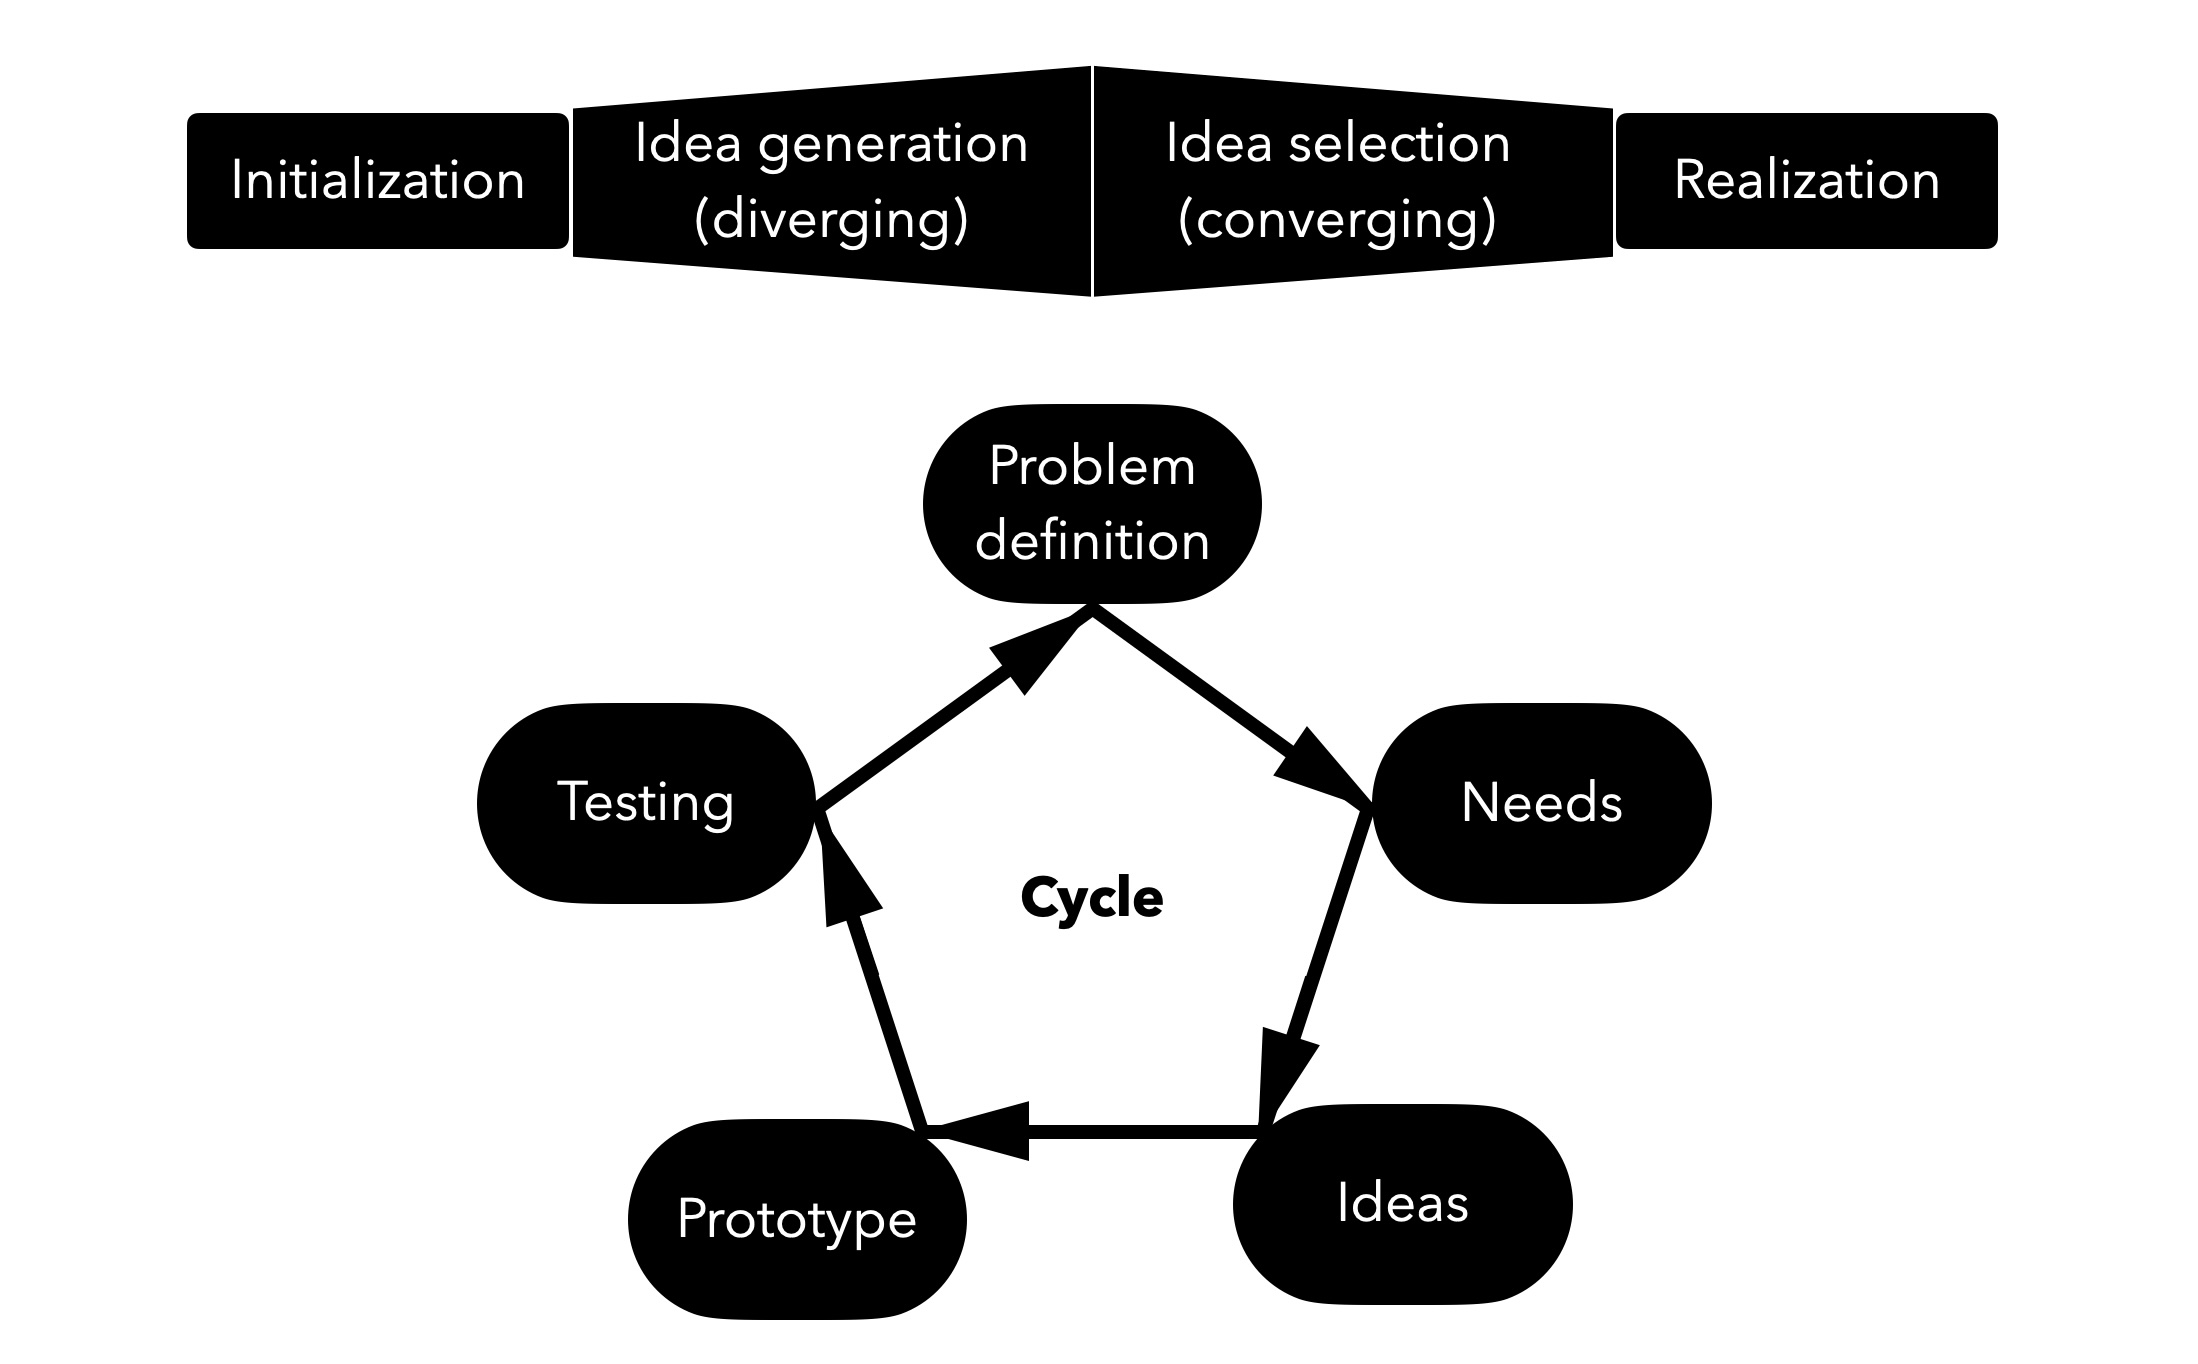
\includegraphics[keepaspectratio,width=13cm]{img/DecisionCycle.jpg}
    \caption{Illustration of the explorative approach, including the stages of initialization, idea generation, idea selection, and implementation. The lower part of the figure shows the decision cycles \autocite{DesignThinking}.}
    \label{fig:decision_cycle}
\end{figure}
\noindent
Teledermatology, especially when focused on Image Quality Assessment (IQA), offers many opportunities for innovation due to the different types of image distortions and ways to address them. To handle this complexity, an exploratory approach was used in this research. This approach is flexible and innovative, allowing for adjustments as new information is discovered, unlike traditional methods like the waterfall approach. \par
\vspace{\baselineskip}
\noindent
At the beginning, the problem was broadly defined, allowing for a flexible and adaptive approach. The research progressed through creative problem-solving with multiple learning cycles, refining ideas and methods iteratively. The project was divided into two main phases. In the \textit{Diverging Phase}, the research question’s scope was expanded to generate new ideas continuously, based on insights from the ongoing literature review. In the \textit{Converging Phase}, the focus on combining these ideas into clear findings and conclusions, aiming to create a unified understanding of the initial problem. This exploratory model is shown in \autoref{fig:decision_cycle}, which illustrates the stages of starting, generating ideas, selecting ideas, and implementation, along with the decision cycles \autocite{DesignThinking}.

\section{Project Control}
\label{sec:ProjectMonitoring}
Even with an exploratory approach, it is important to have a rough timeline to guide the research tasks. A workflow was established before starting, detailed in the planning document attached to this thesis. \par
\noindent
There are three key milestones identified in the first half of the project, each crucial for its success: \par
\vspace{\baselineskip}
\noindent
\textbf{Understanding Teledermatology}: Gaining a thorough understanding of the field to ensure all subsequent actions are relevant and well-informed. \par
\vspace{\baselineskip}
\noindent
\textbf{State of the Art in IQA}: Identifying the latest developments in IQA to ensure the methods used are up-to-date and effective. \par
\vspace{\baselineskip}
\noindent
\textbf{Availability of Teledermatology Data}:  Securing access to appropriate datasets for conducting meaningful IQA. \par
\vspace{\baselineskip}
\noindent
These milestones are essential because each phase of the project relies on the successful completion of the previous one. Missing any of these milestones could significantly impact the project and might require a fundamental reassessment of the objectives outlined in \autoref{sec:Objectives}. \par

\section{Research Steps}
\label{sec:ResearchSteps}
As mentioned, this study was exploratory, so it was not possible to follow a strict, step-by-step process. However, for the individual key steps, I took a systematic approach to stay organized and ensure that each step was done in the right order: \par

\subsection{Literature Review}
\label{sub:LR}
First, I began by getting an overview of my research field. As I was new to the domain of teledermatology and dermatology, this initial step was crucial. By researching and reading relevant literature, I gradually built a solid understanding of the field. Next, I identified the core topics related to my research objectives. Once I had these key topics, I carefully selected the databases to search, focusing on those most relevant to my field: PubMed\footnote{https://pubmed.ncbi.nlm.nih.gov}, Google Scholar\footnote{https://scholar.google.com}, IEEE Xplore\footnote{https://ieeexplore.ieee.org/Xplore/home.jsp}, Connected Papers\footnote{https://www.connectedpapers.com}, and Papers with Code\footnote{https://paperswithcode.com}. Using these databases, I applied search filters to narrow down the results, such as limiting the search to articles published after 2020. \par
\vspace{\baselineskip}
\noindent
I reviewed the titles of the search results and opened the ones that seemed interesting. After that, I read the abstracts to determine their relevance. Depending on the relevance of the abstract and some of the figures, I decided whether to read the full paper. Additionally, for state-of-the-art methods, I focused on finding and reading papers that had published their code and model weights if models were trained. This systematic approach ensured that my literature review was thorough and focused on the most relevant and up-to-date research. \par

\subsection{Data Collection and Preparation}
\label{sub:DataCollection}
In searching for a suitable dataset to evaluate image quality in teledermatology, a major challenge was the lack of Mean Opinion Score (MOS) or Differential Mean Opinion Score (DMOS) in teledermatology datasets, as commonly found in traditional IQA datasets mentioned in \autoref{sub:BenchmarkDatasetsIQA}. This scarcity is due to the resource-intensive nature of labeling images in the medical field. \par
\vspace{\baselineskip}
\noindent
To address this gap, I created a distortion pipeline that synthetically distorts images based on the seven criteria defined in \autoref{sub:QualityCriteriaTeledermatology}. Each type of distortion has five levels of severity, with the severity indicating how poor the image quality is. These distortions are carefully selected to simulate real-world imperfections commonly encountered in teledermatology. Each image is then labeled according to the severity and type of distortion applied, creating a dataset that not only includes the distorted images but also features precise annotations regarding their quality. This allowed me to artificially create labels for my images. For this, I needed high-quality images to start with. I chose two datasets: the SCIN dataset for its relevance and uniqueness, and the Fitzpatrick17k dataset to complement the SCIN dataset. \par
\vspace{\baselineskip}
\noindent
Unlike many dermatology datasets that mainly focus on skin cancer diagnostics by classifying malignant and benign tumors, the SCIN dataset covers a broader range of common dermatological conditions, including allergic, inflammatory, and infectious diseases. These conditions are frequently encountered in everyday clinical practice but are underrepresented in existing datasets. The SCIN dataset is particularly valuable because it captures images of early-stage conditions. Over half of the images were taken less than a week from the onset of symptoms, with 30\% captured less than a day after symptoms appeared \autocite{SCIN}. These are conditions patients are likely to consult via teledermatology platforms before visiting traditional healthcare settings. The Fitzpatrick17k dataset contains more clinical setting images, which provide good quality but do not represent the variability seen in typical teledermatology images \autocite{F17K}, so I used the Fitzpatrick17k dataset only for training purposes. In total, I filtered 475 good quality images from the Fitzpatrick17k dataset and another 475 good quality images from the SCIN dataset, along with 200 randomly selected test images from the SCIN dataset.\par
\vspace{\baselineskip}
\noindent
This approach to dataset preparation not only tailored the data to the specific needs of this research but also established a framework for systematically assessing image quality in teledermatology. This preparation is crucial for the next phases of the project, which involve training and validating the image quality assessment model to ensure it can reliably perform in real-world teledermatology applications. \par

\subsection{Feature Extraction}
\label{sub:FeatureExtraction}
Feature extraction is the next important step where the SimCLR model from ARNIQA is used to identify key features from the distorted images. These features capture the patterns of distortions that affect image quality. The extracted features and the generated labels are then used to train different models, including XGBoost regressor, XGBoost classifier, and MLP regressor, to see which one works best for assessing image quality. \par

\subsection{Training and Validation}
\label{sub:TrainVal}
The training of the models is based on the prepared training data. Since I am generating labels and distorted images, I am not restricted by the original amount of data. I can run the images through the distortion pipeline multiple times, creating various versions of distortions from the original images. The models are then trained with these data to develop their ability to assess image quality. Validation is done in parallel with training by using a portion of the data as a validation set. This helps evaluate and monitor the performance of the models. \par 


\subsection{Testing and Experiments}
\label{sub:TestExperiment}
After completing the training, the models are evaluated using independent test data. I labeled 200 test images, scoring each one on the seven quality criteria to ensure the model’s performance can be compared to human evaluation. This phase is crucial to assess the actual performance and reliability of the models. The evaluation is conducted using defined metrics such as Precision, Recall, Spearman’s Rank Order Correlation Coefficient (SRCC), and Pearson Linear Correlation Coefficient (PLCC). The results of this evaluation provide valuable insights into the strengths and weaknesses of the image quality assessment models and serve as a basis for further improvements or adjustments. \par 

\subsection{Discussion and Further Development}
\label{sub:DiscussionDevelopment}
In conclusion, the results of the project are analyzed and discussed. This discussion includes an evaluation of the achieved goals, an analysis of the challenges and limitations of the project, and a look at possible further developments. Additionally, potential applications of the developed image quality assessment models in teledermatology are considered, along with the opportunities and challenges that arise from these applications. \par

\chapter{Implementation}
\label{ch:Implementation}
text

\chapter{Results and Analysis}
\label{ch:ResultsAnalysis}
In this chapter, the performance of the trained models is analyzed and discussed. The main focus is on the final MLP regressor model, which was found to be the best performing model across multiple criteria. The selection of the MLP regressor is supported by the results shown in \autoref{fig:ModelSRCC}, which presents a parallel coordinate plot comparing the best-performing models across all seven criteria and the overall SRCC.\par
The parallel coordinate plot shows that the MLP regressor consistently performs better than the other models across all criteria. Although all models perform similarly for different criteria, no model stands out in a specific criterion. This could be because the same features were used for every criterion, with only the target labels differing. \par
\vspace{\baselineskip}
\noindent
In addition to the parallel coordinate plot, \autoref{table:srcc_results} summarizes the cross-dataset evaluation results, showing the generalizability of the models. The table lists the models in the left column and their evaluation results on the SCIN and Fitzpatrick (F17K) datasets in the right columns. This table shows how well the models, trained on one dataset, perform when evaluated on another, providing insights into their robustness and adaptability. All data were synthetically distorted through the pipeline to ensure consistent evaluation conditions. \par
\vspace{\baselineskip}
\noindent
Given these findings, the MLP regressor was chosen as the final model for further testing. The following sections will detail the performance of the MLP regressor on the test images, providing a clear analysis of its strengths and weaknesses in assessing image quality in teledermatology. \par

\section{Range of Distortion Values}
\label{sec:RangeDistortionValues}
The ranges of values for each distortion type were carefully chosen to reflect realistic scenarios for teledermatology  applications. Each distortion type was visualized individually to make sure they were appropriate. \autoref{sec:Degradation_Types} includes images that show each criterion with different distortion types and five severity levels. \par
\vspace{\baselineskip}
\noindent
It is important to note that images should not be normalized before viewing because normalization can make the images appear overly colorful and unrealistic. However, normalization is necessary during training and testing because the feature extraction backbone from ARNIQA\autocite{ARNIQA} was trained on ResNet50 with ImageNet images. This step helps the model accurately extract relevant features from the images. \par
\section{Model Performance}
\label{sec:ModelPerformance}
To fully understand the performance of the four different models with different architectures, a cross-dataset evaluation was done. \autoref{table:srcc_results} summarizes the overall Spearman’s Rank Correlation Coefficient (SRCC) on the synthetically distorted SCIN and Fitzpatrick datasets. This evaluation highlights how well the models generalize across different datasets. Note that the Fitzpatrick dataset is referred to as F17K for simplicity. \par 
\begin{table}[h]
    \centering
    \begin{tabular}{|l|c|c|}
        \hline
        \textbf{Model} & \textbf{SCIN} & \textbf{F17K} \\
        \hline
        Combined MLP Regressor & \underline{0.66} & \underline{0.75} \\
        Combined XGB Regressor & 0.65 & 0.73 \\
        Combined XGB Classifier & 0.58 & 0.61 \\
        Combined MLP Classifier & 0.43 & 0.46 \\
        \hline
        F17K MLP Regressor & 0.54 & 0.69 \\
        SCIN MLP Regressor & 0.62 & 0.49 \\
        F17K XGB Regressor & 0.53 & 0.67 \\
        SCIN XGB Regressor & 0.61 & 0.48 \\
        SCIN MLP Classifier & 0.53 & 0.45 \\
        F17K MLP Classifier & 0.47 & 0.58 \\
        SCIN XGB Classifier & 0.54 & 0.43 \\
        F17K XGB Classifier & 0.46 & 0.59 \\
        \hline
    \end{tabular}
    \caption{Spearman’s Rank Correlation Coefficient (SRCC) of Different Models on SCIN and F17K Datasets. F17K refers to the Fitzpatrick17k dataset.}
    \label{table:srcc_results}
\end{table}
\subsection{Parallel Coordinate Plot}
\label{subsec:ParallelCoordinatePlot}
\autoref{fig:ModelSRCC}, a parallel coordinate presents a visual comparison of the model performances across different criteria and the overall SRCC. \par
\begin{figure}[ht]
    \centering
    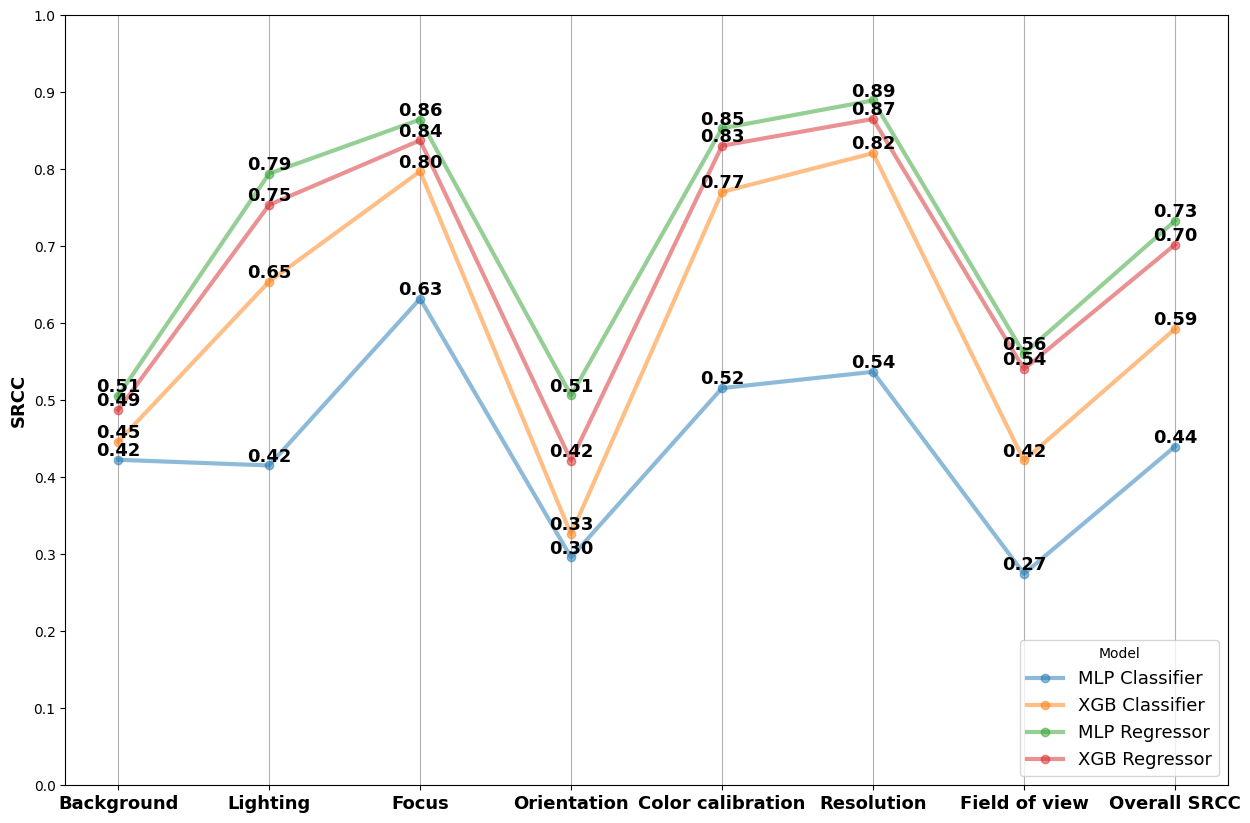
\includegraphics[keepaspectratio,width=15cm]{img/Model_SRCC.png}
    \caption{Parallel coordinate plot showing the best SRCC values for the four different models across the seven criteria and the overall SRCC. This plot highlights the performance of the MLP Regressor.}
    \label{fig:ModelSRCC}
\end{figure}

\subsection{Performance Metrics}
\label{subsec:PerformanceMetrics}
The performance of the final MLP regressor model on individual criteria is shown in \autoref{table:performance_metrics}. This table provides a comprehensive view of the model’s strengths and weaknesses, highlighting areas for improvement. The model was evaluated on 475 good quality Fitzpatrick images that were synthetically distorted using the distortion pipeline. \par
\begin{table}[h]
    \centering
    \begin{tabular}{|l|c|c|c|c|}
        \hline
        \textbf{Criteria} & \textbf{MAE} & \textbf{R\textsuperscript{2}} & \textbf{SRCC} & \textbf{Cohen's Kappa} \\
        \hline
        Background & 0.9684 & 0.2595 & 0.5422 & 0.4399 \\
        Lighting & 0.5726 & 0.6440 & 0.8028 & 0.7913 \\
        Focus & 0.4042 & 0.7385 & 0.8622 & 0.8568 \\
        Orientation & 0.9895 & 0.1824 & 0.4735 & 0.4102 \\
        Color calibration & 0.4905 & 0.7334 & 0.8622 & 0.8583 \\
        Resolution & 0.3642 & 0.7656 & 0.8722 & 0.8726 \\
        Field of view & 0.5474 & 0.5976 & 0.7710 & 0.7660 \\
        \hline
        \textbf{Overall} & \textbf{0.6195} & \textbf{0.5646} & \textbf{0.7507} & \textbf{0.7396} \\
        \hline
    \end{tabular}
    \caption{Performance Metrics for Each Distortion Criteria}
    \label{table:performance_metrics}
\end{table}

\clearpage
\subsection{Confusion Matrices}
\label{subsec:ConfusionMatrices}
In addition to numerical metrics, confusion matrices\footnote{from utils.visualization import plot\_all\_confusion\_matrices} were created for each criterion, as shown in \autoref{fig:confusion_matrices}. These matrices display where the model makes correct predictions and where it makes mistakes, showing a detailed view of its accuracy for each type of distortion. The comparison between actual and predicted scores helps identify specific areas where the model performs well and areas that need improvement. Furthermore, the confusion matrices also reveal any biases the model might have toward certain severity ranges, indicating whether it tends to predict only low or high severity levels, or if its predictions are skewed in some way. \par
\vspace{\baselineskip}
\begin{figure}[ht]
    \centering
    \begin{subfigure}[b]{0.32\textwidth}
        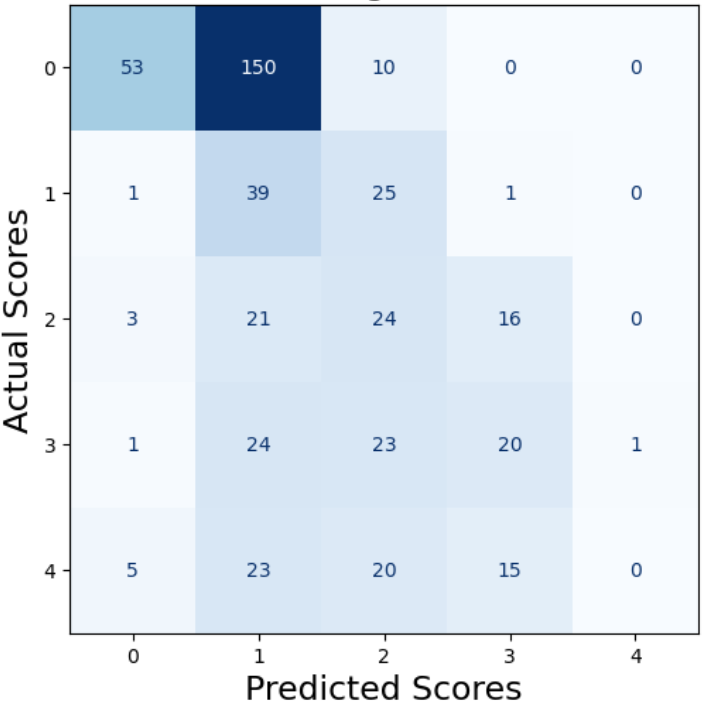
\includegraphics[width=\textwidth]{img/cm/bg.png}
        \caption{Background}
        \label{fig:cm_bg}
    \end{subfigure}
    \hfill
    \begin{subfigure}[b]{0.32\textwidth}
        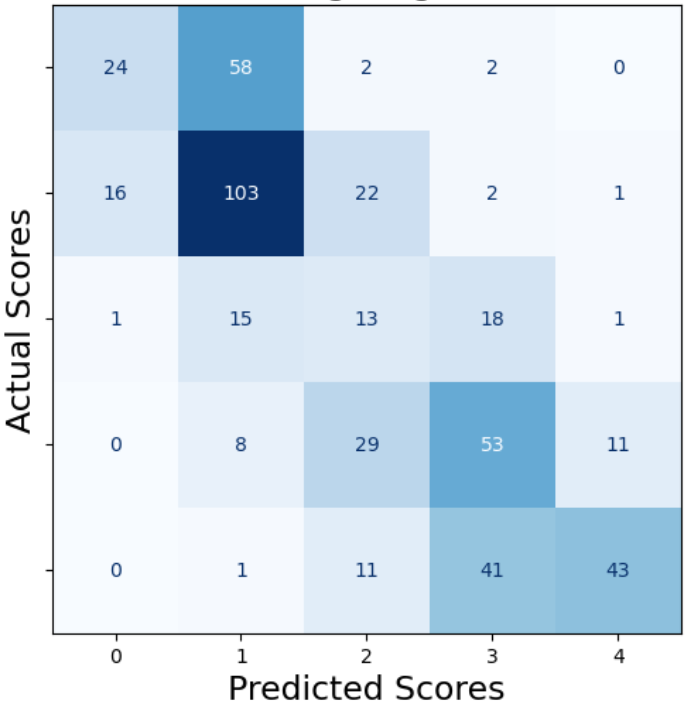
\includegraphics[width=\textwidth]{img/cm/light.png}
        \caption{Lighting}
        \label{fig:cm_light}
    \end{subfigure}
    \hfill
    \begin{subfigure}[b]{0.32\textwidth}
        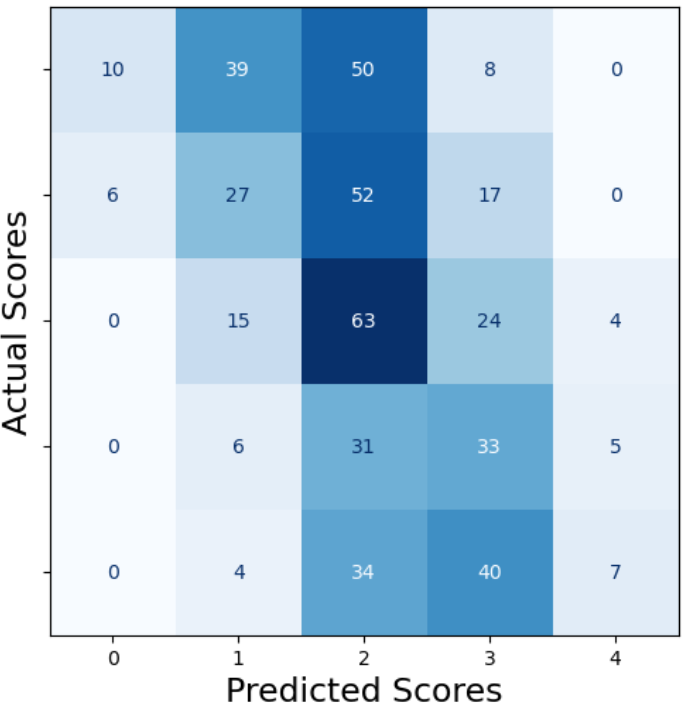
\includegraphics[width=\textwidth]{img/cm/orient.png}
        \caption{Orientation}
        \label{fig:cm_orient}
    \end{subfigure} 

    \begin{subfigure}[b]{0.24\textwidth}
        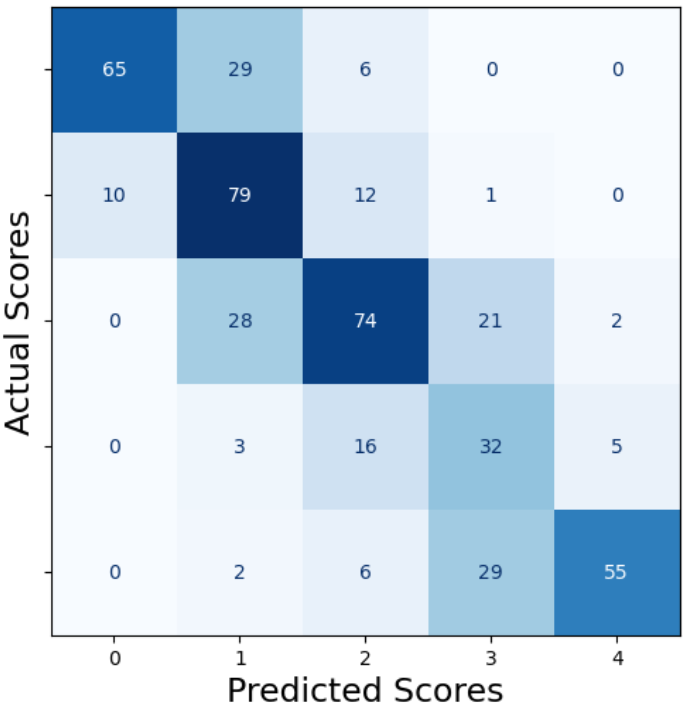
\includegraphics[width=\textwidth]{img/cm/foc.png}
        \caption{Focus}
        \label{fig:cm_foc}
    \end{subfigure}
    \hfill
    \begin{subfigure}[b]{0.24\textwidth}
        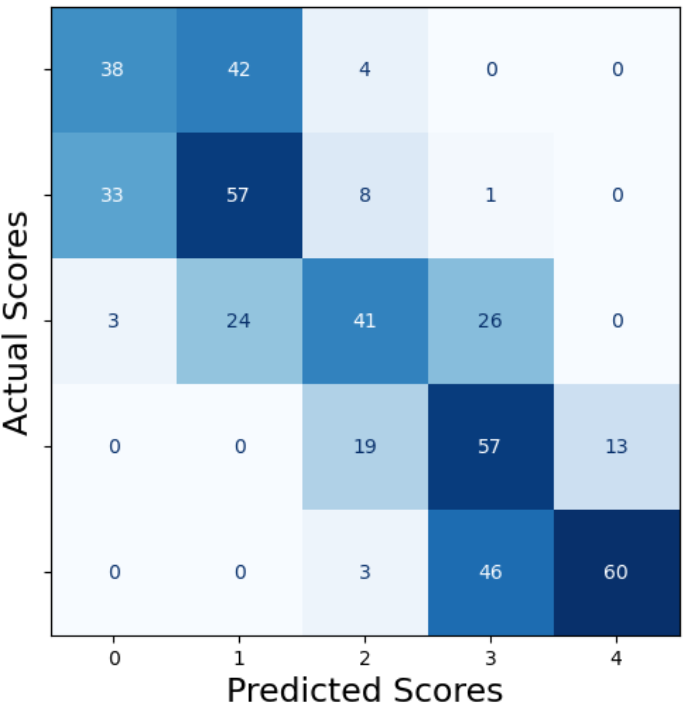
\includegraphics[width=\textwidth]{img/cm/cc.png}
        \caption{Color Calibration}
        \label{fig:cm_cc}
    \end{subfigure}
    \hfill
    \begin{subfigure}[b]{0.24\textwidth}
        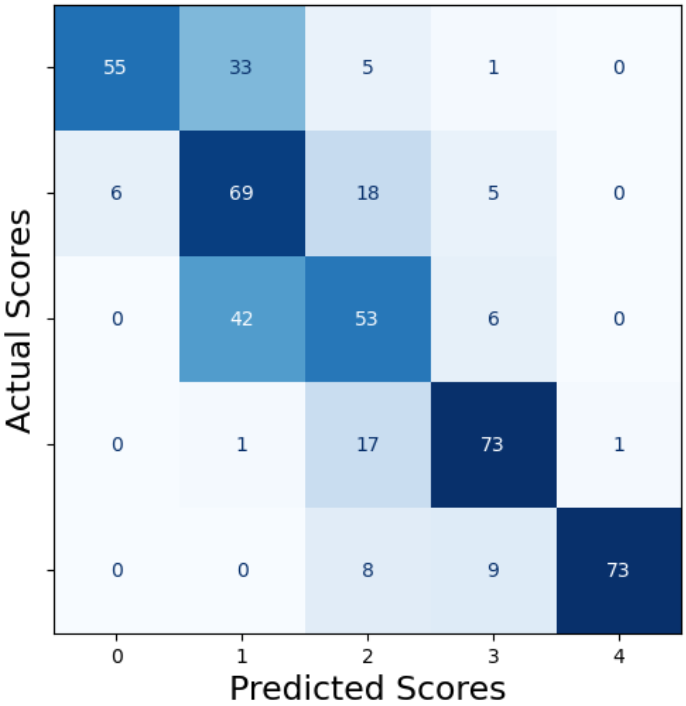
\includegraphics[width=\textwidth]{img/cm/res.png}
        \caption{Resolution}
        \label{fig:cm_res}
    \end{subfigure}
    \hfill
    \begin{subfigure}[b]{0.24\textwidth}
        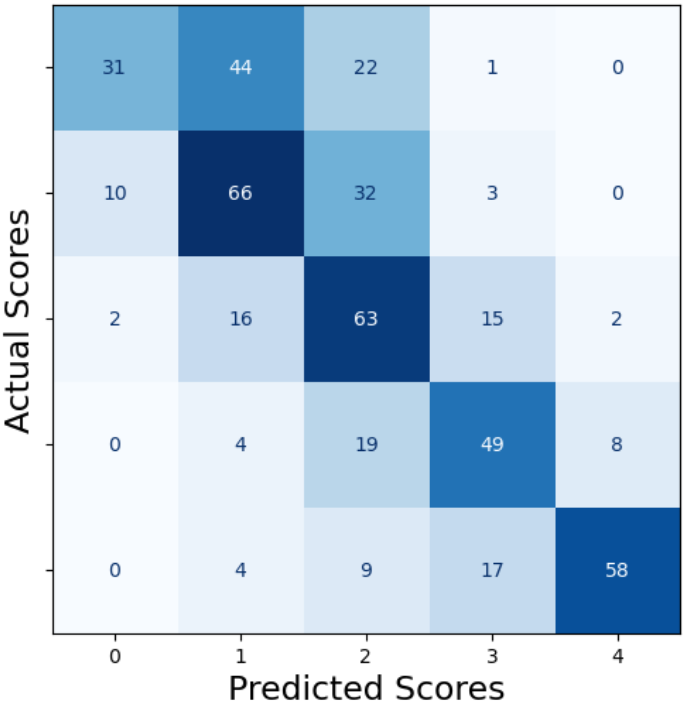
\includegraphics[width=\textwidth]{img/cm/fov.png}
        \caption{Field of View}
        \label{fig:cm_fov}
    \end{subfigure}
    \caption{Confusion matrices for the MLP Regressor model evaluated on the 475 images from the Fitzpatrick dataset. Each matrix corresponds to a specific distortion criterion and shows the actual scores on the y-axis and the predicted scores on the x-axis. Darker shades indicate higher counts, highlighting where the model's predictions match the actual values and where discrepancies occur.}
    \label{fig:confusion_matrices}
\end{figure}
\vspace{\baselineskip}
\noindent

\clearpage
\section{Model Predictions}
\label{sec:VisualizingPredictions}
To better understand the model’s performance on the two test sets (70 synthetic distorted images and 200 authentic images), radar charts\footnote{from utils.visualization import plot\_results} were created. These charts show the criteria on the outside, with severity ranges going from the center (0) to the outer edge (1), indicating high distortion for each criterion. These visualizations provide a clear and simple view of the model’s performance, showing its strengths and areas for improvement. They help identify specific cases where the model predicted the correct severity and where it struggled. The radar charts also make it easy to see which distortions the model handles well and which need more attention. \par
\subsection{Visualizations for Synthetic Distorted Images}
\label{subsec:SyntheticDistortedImages}
These visualizations, as shown in \autoref{fig:synthetic}, help to compare the model's predictions with the actual distortions introduced by the pipeline. This approach clearly demonstrates the model's ability to handle various types of distortions. \par
\vspace{\baselineskip}
\noindent
The first column shows the original image, the second displays the distorted image, the third contains the actual labels, and the fourth presents the model’s predictions. This setup makes it easy to compare the model’s predictions with the actual distortions. \par
\begin{figure}[ht]
    \centering
    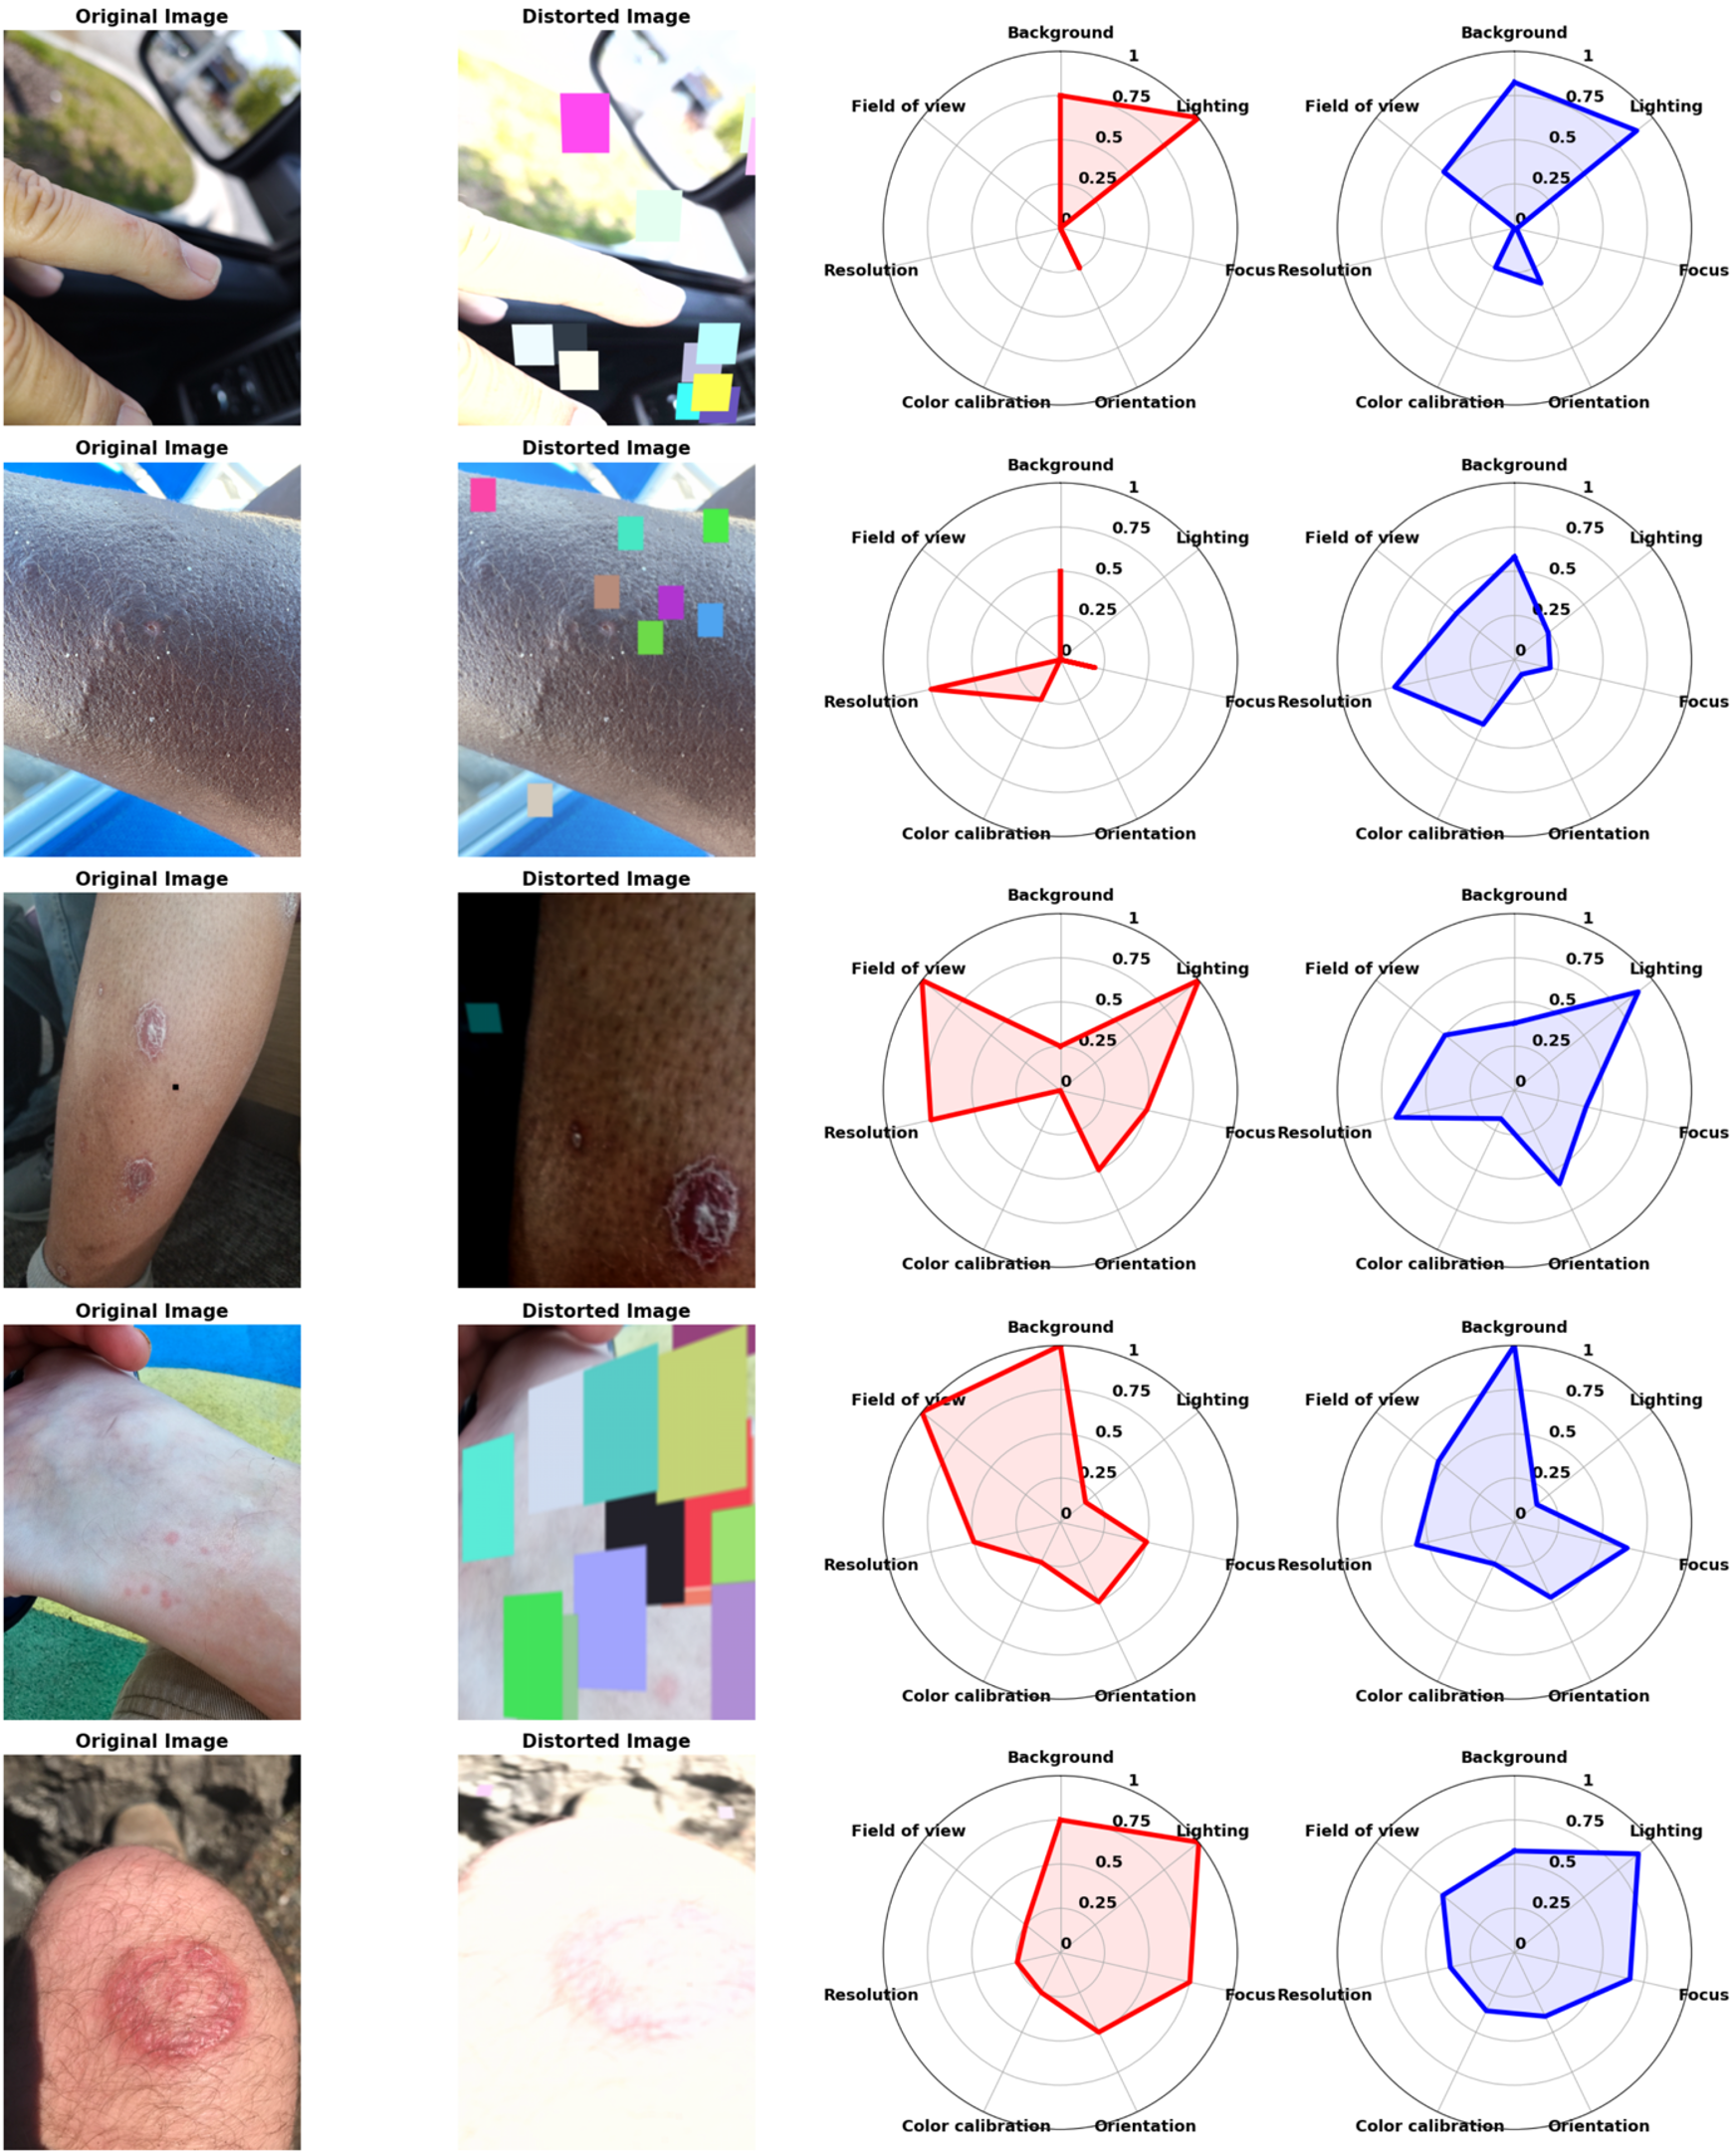
\includegraphics[keepaspectratio,width=15cm]{img/synthetic.png}
    \caption{Visualizations for the MLP Regressor model on 70 synthetic distorted images. The four-column layout shows the original image, the distorted image, the actual labels, and the model's predictions.}
    \label{fig:synthetic}
\end{figure}

\subsection{Visualizations for Authentic Images}
\label{subsec:AuthenticImages}
The visualizations, as shown in \autoref{fig:authentic}, compare the model's predictions with human-labeled scores. This method highlights the model's performance in real-world scenarios, showing its strengths and areas for improvement. \par
\vspace{\baselineskip}
\noindent
The first column shows the image, the second column displays the human-labeled scores, and the third column presents the model’s predictions. This comparison helps show how well the model’s predictions align with the human evaluations. \par
\begin{figure}[ht]
    \centering
    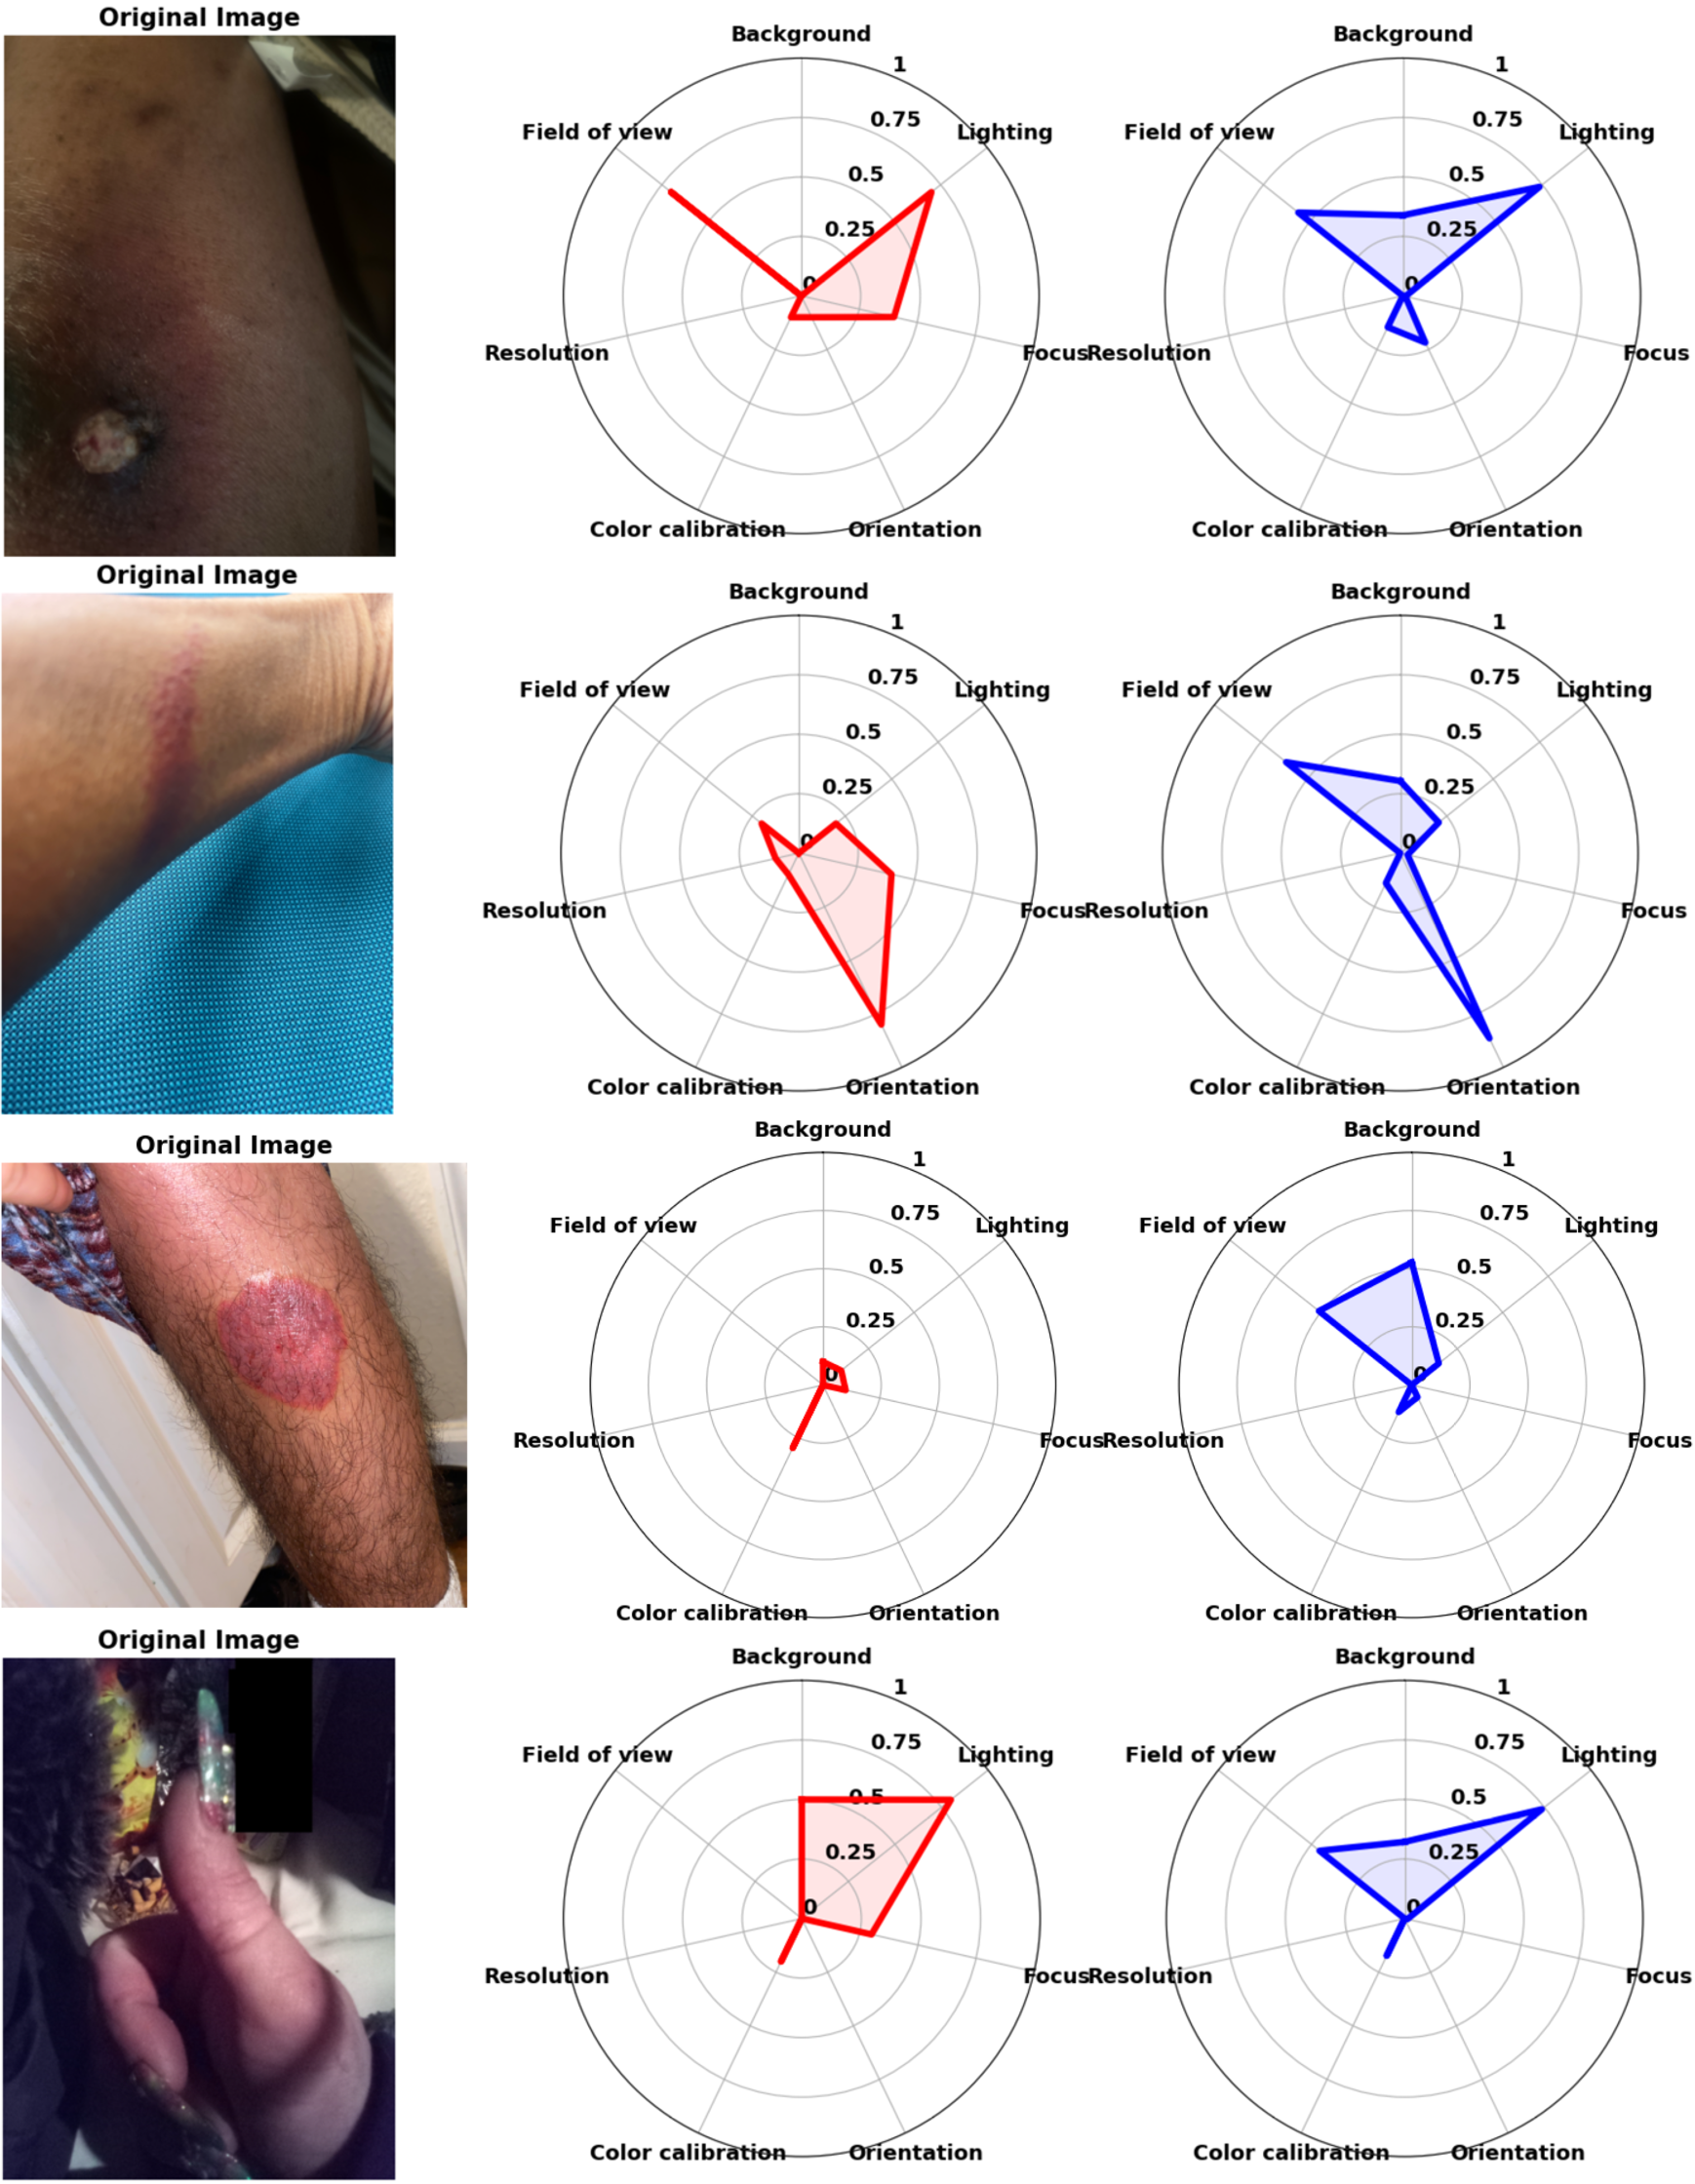
\includegraphics[keepaspectratio,width=15cm]{img/authentic.png}
    \caption{Visualizations for the MLP Regressor model on 200 authentic images. The three-column layout shows the image, the human-labeled scores, and the model's predictions.}
    \label{fig:authentic}
\end{figure}
\clearpage
\section{Assessing Training and Testing Images Quality}
\label{sec:TestingFilteredImages}
To verify the quality of the images used for training and see how they change after synthetic distortion, radar charts were created. These charts show the quality of the original training images and how they are affected by the distortions. Additionally, the quality of both the synthetic and authentic test images is assessed using the same method. These radar charts show a simple visual representation of the quality and the level of distortion across the seven criteria. \par
\subsection{Training Images Quality}
\label{subsec:TrainingImagesQuality}
\subsubsection{SCIN Dataset}
\label{subsubsec:SCINDataset}
\begin{figure}[ht]
    \centering
    \begin{subfigure}[b]{0.48\textwidth}
        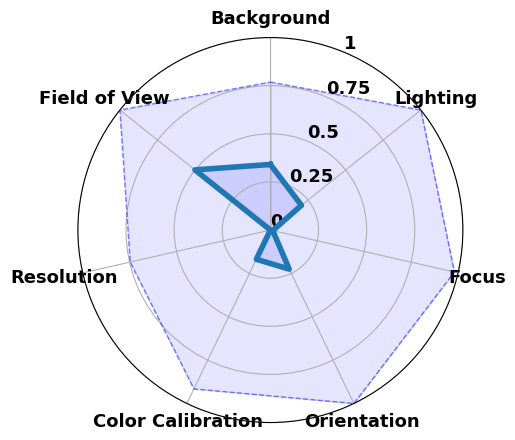
\includegraphics[width=\textwidth]{img/hept/SCIN10k.png}
        \caption{SCIN Images}
        \label{fig:SCIN10k}
    \end{subfigure}
    \hfill
    \begin{subfigure}[b]{0.48\textwidth}
        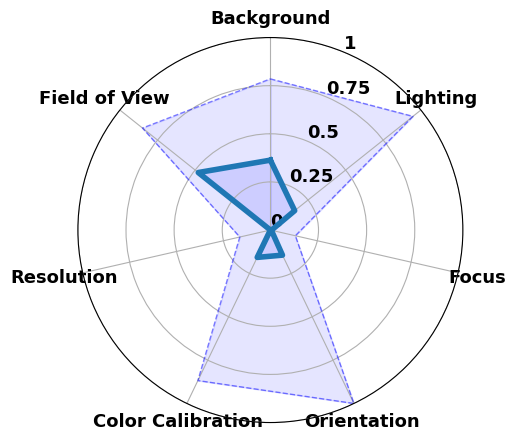
\includegraphics[width=\textwidth]{img/hept/SCIN.png}
        \caption{Filtered SCIN Images}
        \label{fig:SCIN}
    \end{subfigure}
    \hfill
    \caption{Radar charts for the SCIN dataset. (a) Original images from the SCIN dataset (10'379 images). (b) Filtered good quality images (475 images).}
    \label{fig:SF}
\end{figure}
\clearpage
\subsubsection{Fitzpatrick Dataset}
\label{subsubsec:FitzpatrickDataset}
\begin{figure}[ht]
    \centering
    \begin{subfigure}[b]{0.48\textwidth}
        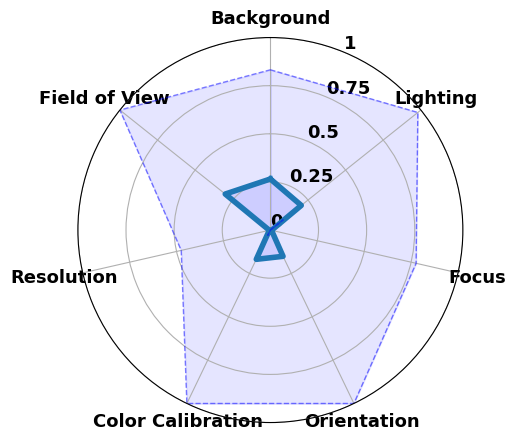
\includegraphics[width=\textwidth]{img/hept/Fitzpatrick17k.png}
        \caption{Fitzpatrick Images}
        \label{fig:Fitzpatrick17K}
    \end{subfigure}
    \hfill
    \begin{subfigure}[b]{0.48\textwidth}
        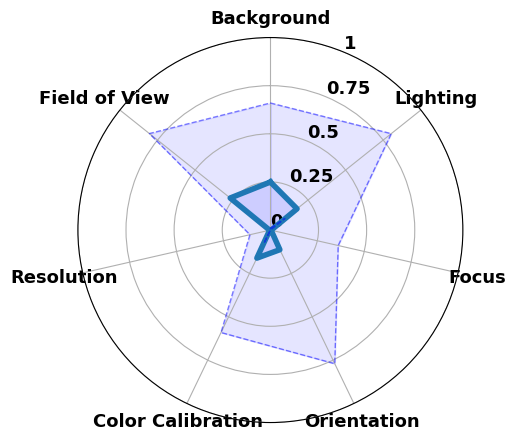
\includegraphics[width=\textwidth]{img/hept/F17K.png}
        \caption{Filtered Fitzpatrick Images}
        \label{fig:F17K}
    \end{subfigure}
    \hfill
    \caption{Radar charts for the Fitzpatrick dataset. (a) Original images from the Fitzpatrick dataset (16'577 images). (b) Filtered good quality images (475 images).}
    \label{fig:FF}
\end{figure}

\subsubsection{Combined Dataset}
\label{subsubsec:CombinedDataset}
\begin{figure}[ht]
    \centering
    \begin{subfigure}[b]{0.48\textwidth}
        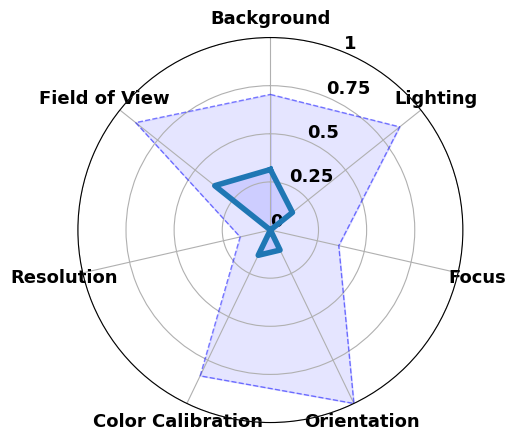
\includegraphics[width=\textwidth]{img/hept/combined.png}
        \caption{Combined SCIN and Fitzpatrick Images}
        \label{fig:combined}
    \end{subfigure}
    \hfill
    \begin{subfigure}[b]{0.48\textwidth}
        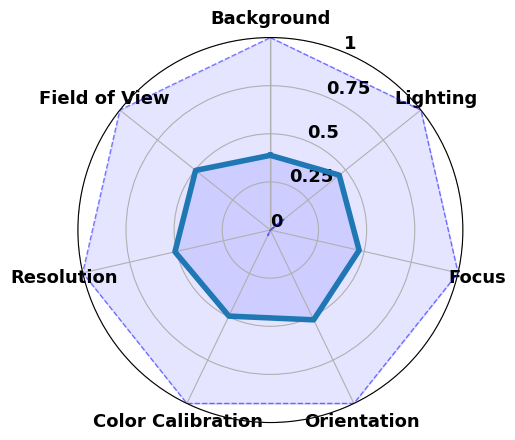
\includegraphics[width=\textwidth]{img/hept/comb_synthetic.png}
        \caption{Synthetically Distorted Images}
        \label{fig:comb_synthetic}
    \end{subfigure}
    \hfill
    \caption{Combined dataset analysis. (a) Combined SCIN and Fitzpatrick images (950 images). (b) Synthetically distorted images.}
    \label{fig:CF}
\end{figure}
\clearpage
\subsection{Test Images Quality}
\label{subsec:TestImagesQuality}
\subsubsection{Synthetic Test Images}
\label{subsubsec:SyntheticTestImages}
\begin{figure}[ht]
    \centering
    \begin{subfigure}[b]{0.48\textwidth}
        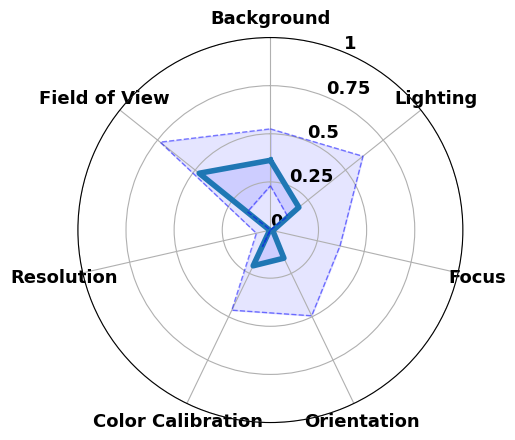
\includegraphics[width=\textwidth]{img/hept/test_70.png}
        \caption{Filtered Test Images}
        \label{fig:test_70}
    \end{subfigure}
    \hfill
    \begin{subfigure}[b]{0.48\textwidth}
        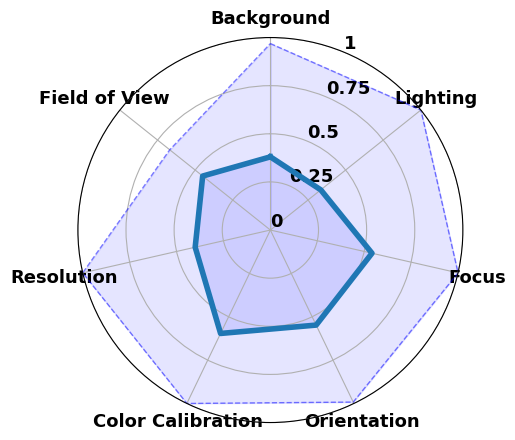
\includegraphics[width=\textwidth]{img/hept/test_70_synthetic.png}
        \caption{Synthetically Distorted Test Images}
        \label{fig:test_70_synthetic}
    \end{subfigure}
    \hfill
    \caption{Synthetic test set analysis. (a) Filtered good quality test images (70 images, independent of training set). (b) Synthetically distorted test images.}
    \label{fig:T1}
\end{figure}

\subsubsection{Authentic Test Images}
\label{subsubsec:AuthenticTestImages}
\begin{figure}[ht]
    \centering
    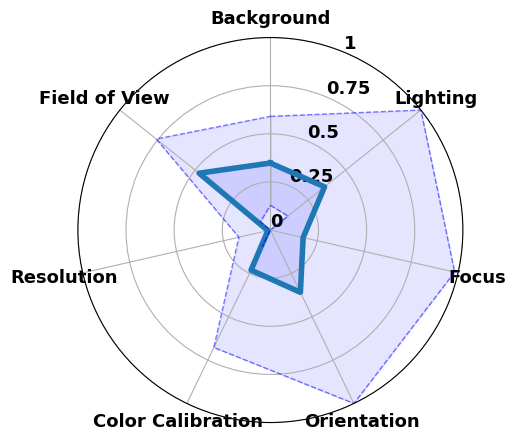
\includegraphics[keepaspectratio,width=7cm]{img/hept/test_200.png}
    \caption{Authentic test set from the SCIN dataset, independent of the training images, showing real-world distortions.}
    \label{fig:T2}
\end{figure}

\chapter{Conclusion and Future Work}
\label{ch:DiscussionConclusion}
text


%\chapter{Chapter}
\label{ch:Chapter}
text

\section{Section}
\label{sec:Section}
text \par
\vspace{\baselineskip}
\noindent

\newpage

\pagenumbering{Roman}

\appendix
% Verhindert das Einfügen von Kapiteltitel kleiner als \chapter
\addtocontents{toc}{\protect\setcounter{tocdepth}{0}}

%\printglossary

%\listofmyequations \pagebreak

\printbibliography

\chapter{Supplementary Material}
\label{ch:Supplementary}

The following pages contain the supplementary material for this thesis. This section includes documents specific to project planning and management. The documents are attached in this order: \par

\begin{itemize}
    \item Project Assignment
    \item Risk Management
    \item Project Planning
\end{itemize}
\vspace{\baselineskip}
\noindent
Additionally, the appendix contains detailed information on the IQA databases from the general image domain, showcases the different dermatology quality criteria and their types across five severity ranges, and provides an overview of the proposed framework for automated IQA in teledermatology. \par

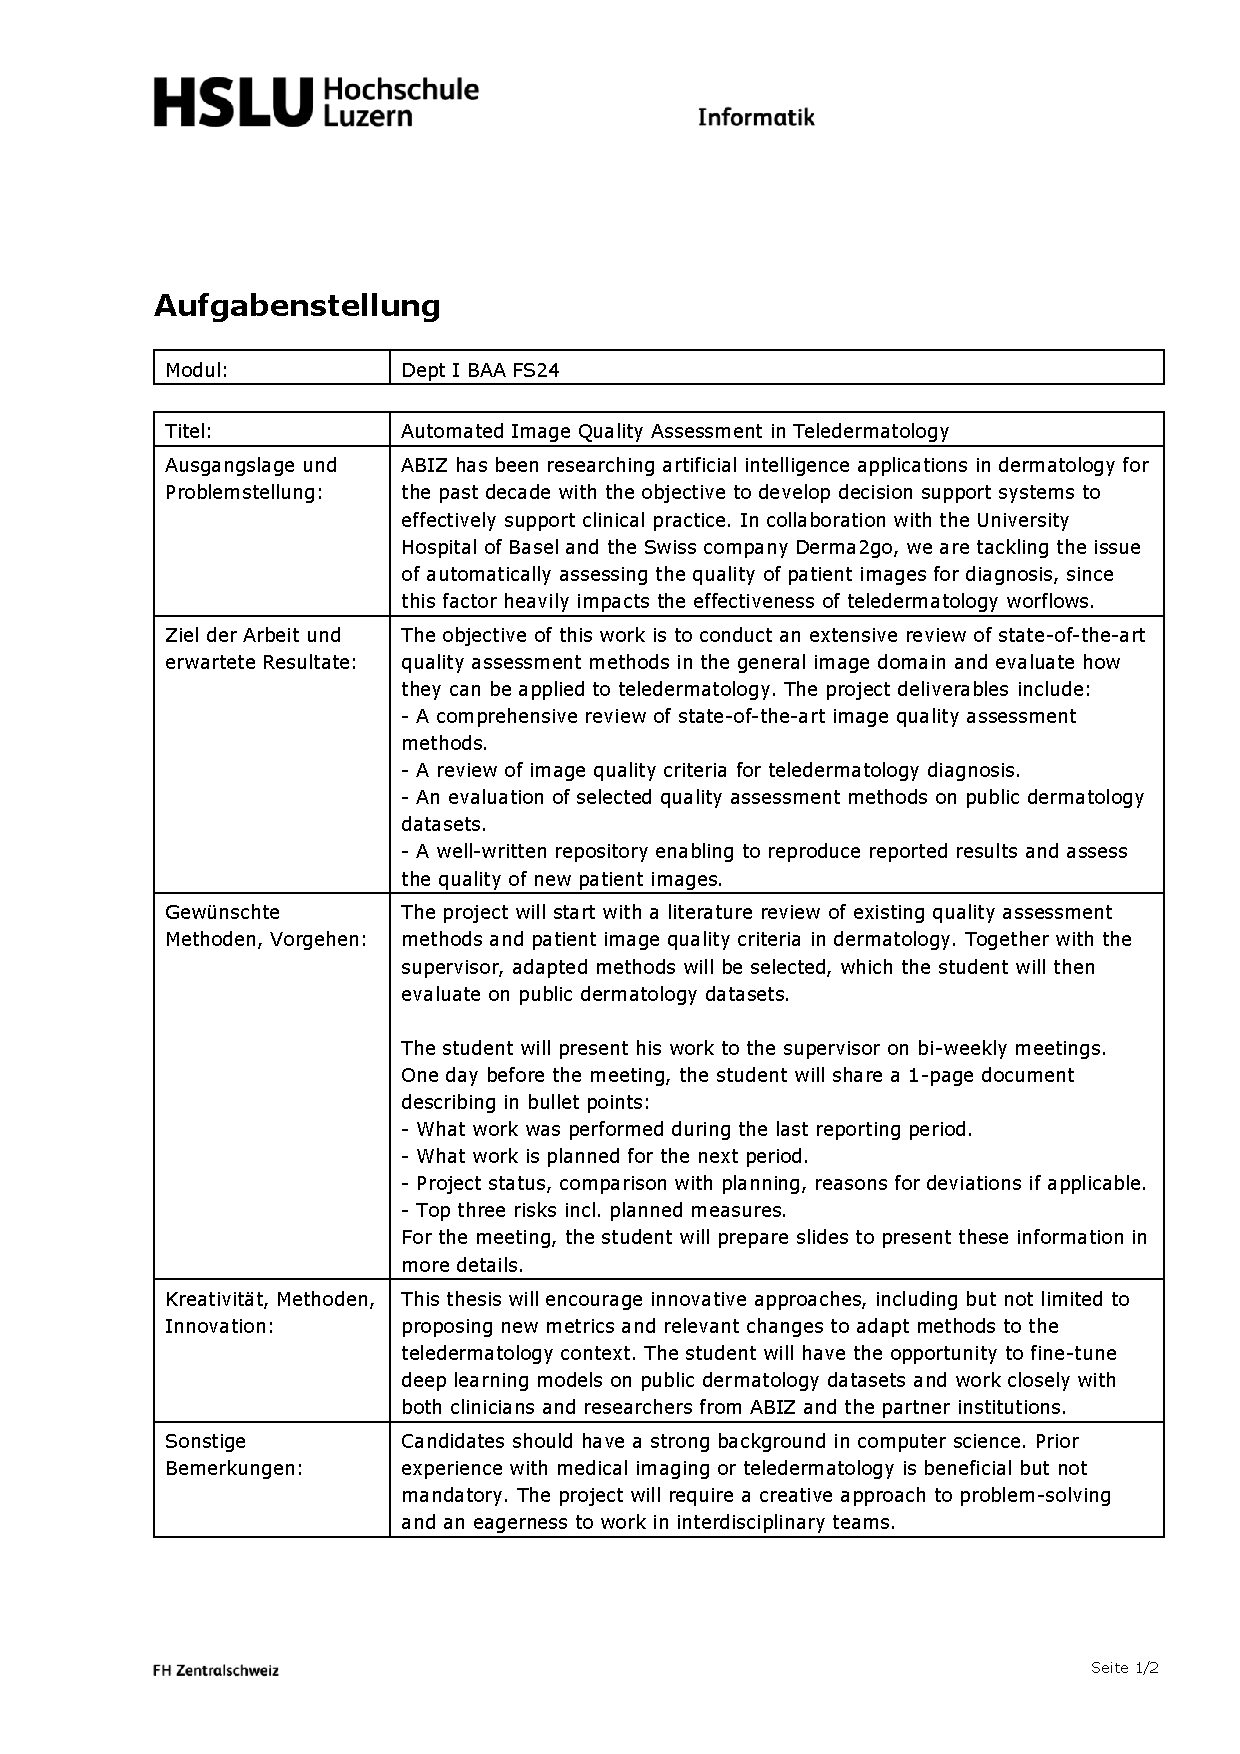
\includepdf[pages=-]{Aufgabenstellung_BAA.pdf}
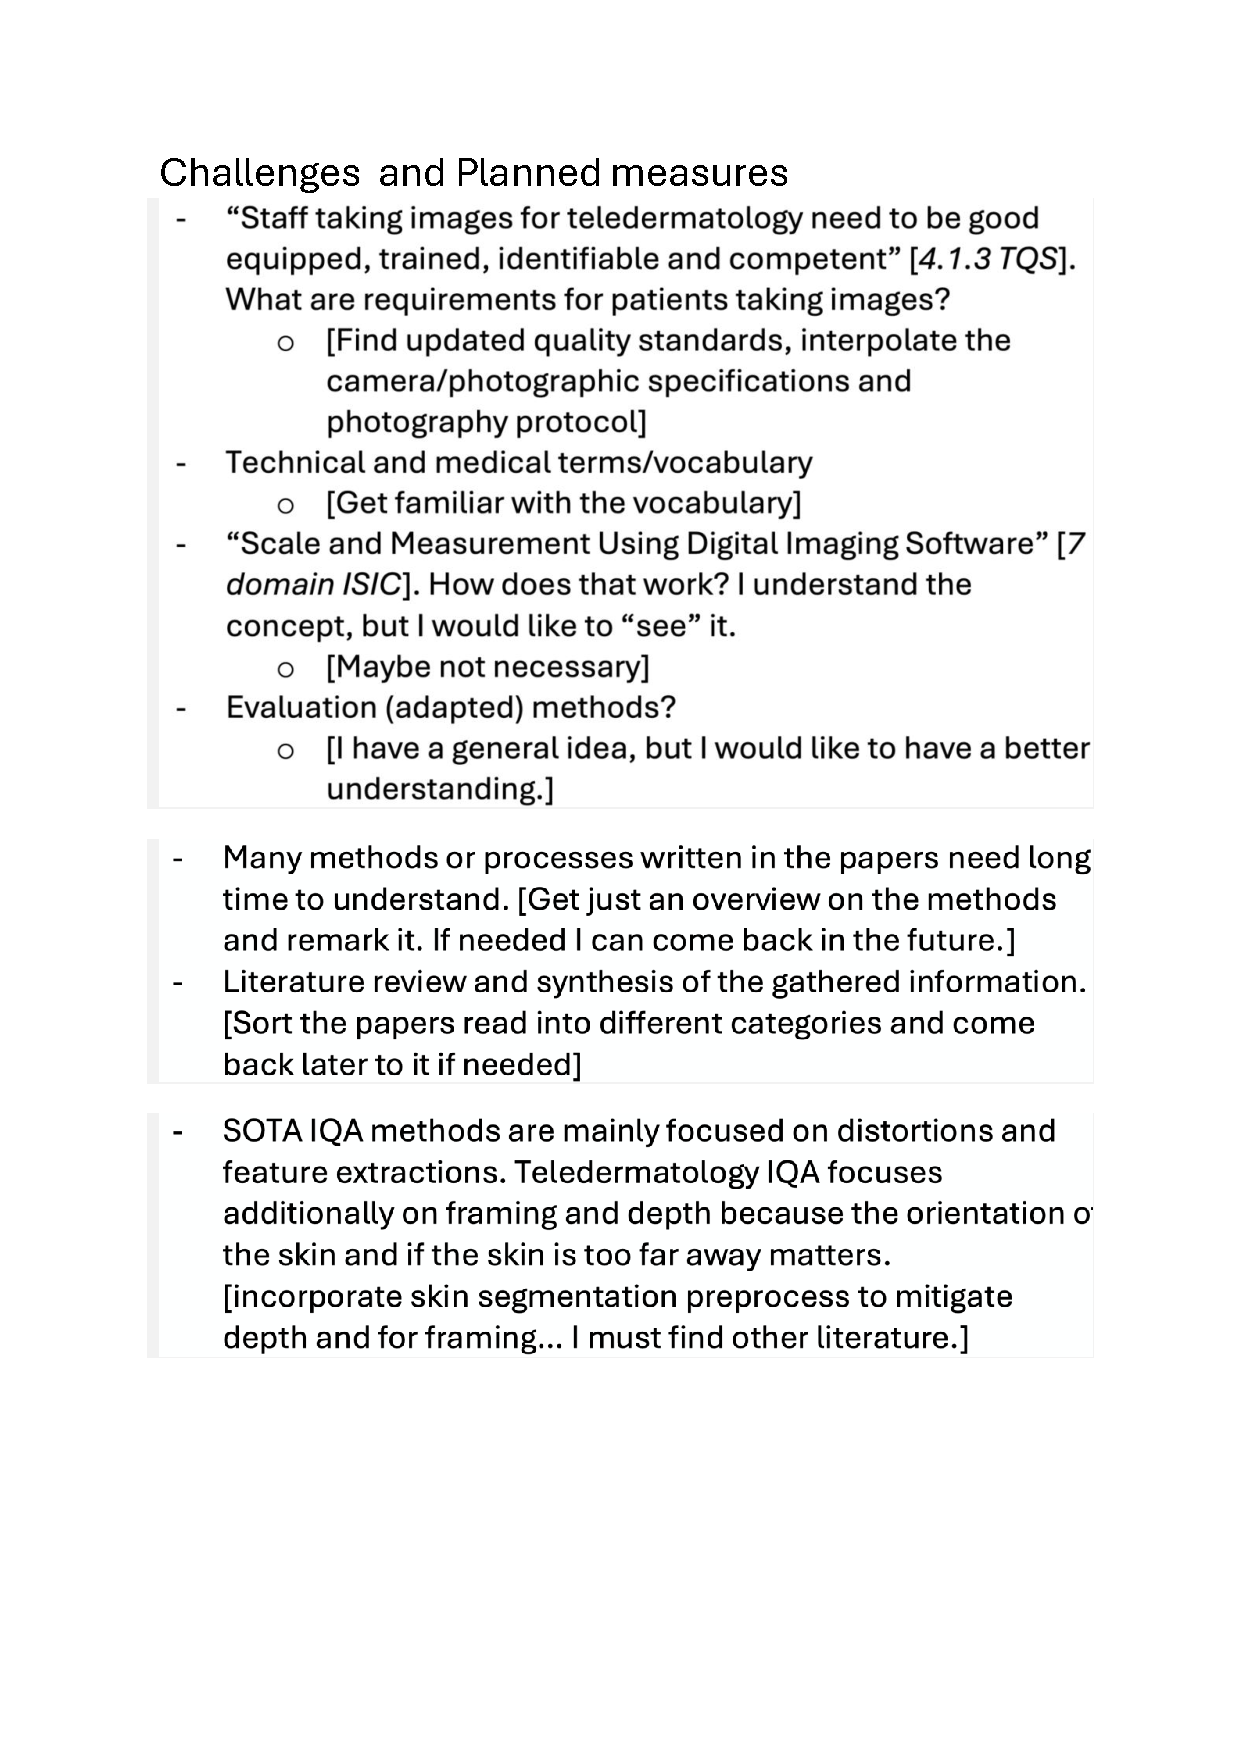
\includepdf[pages=-]{challenges.pdf}
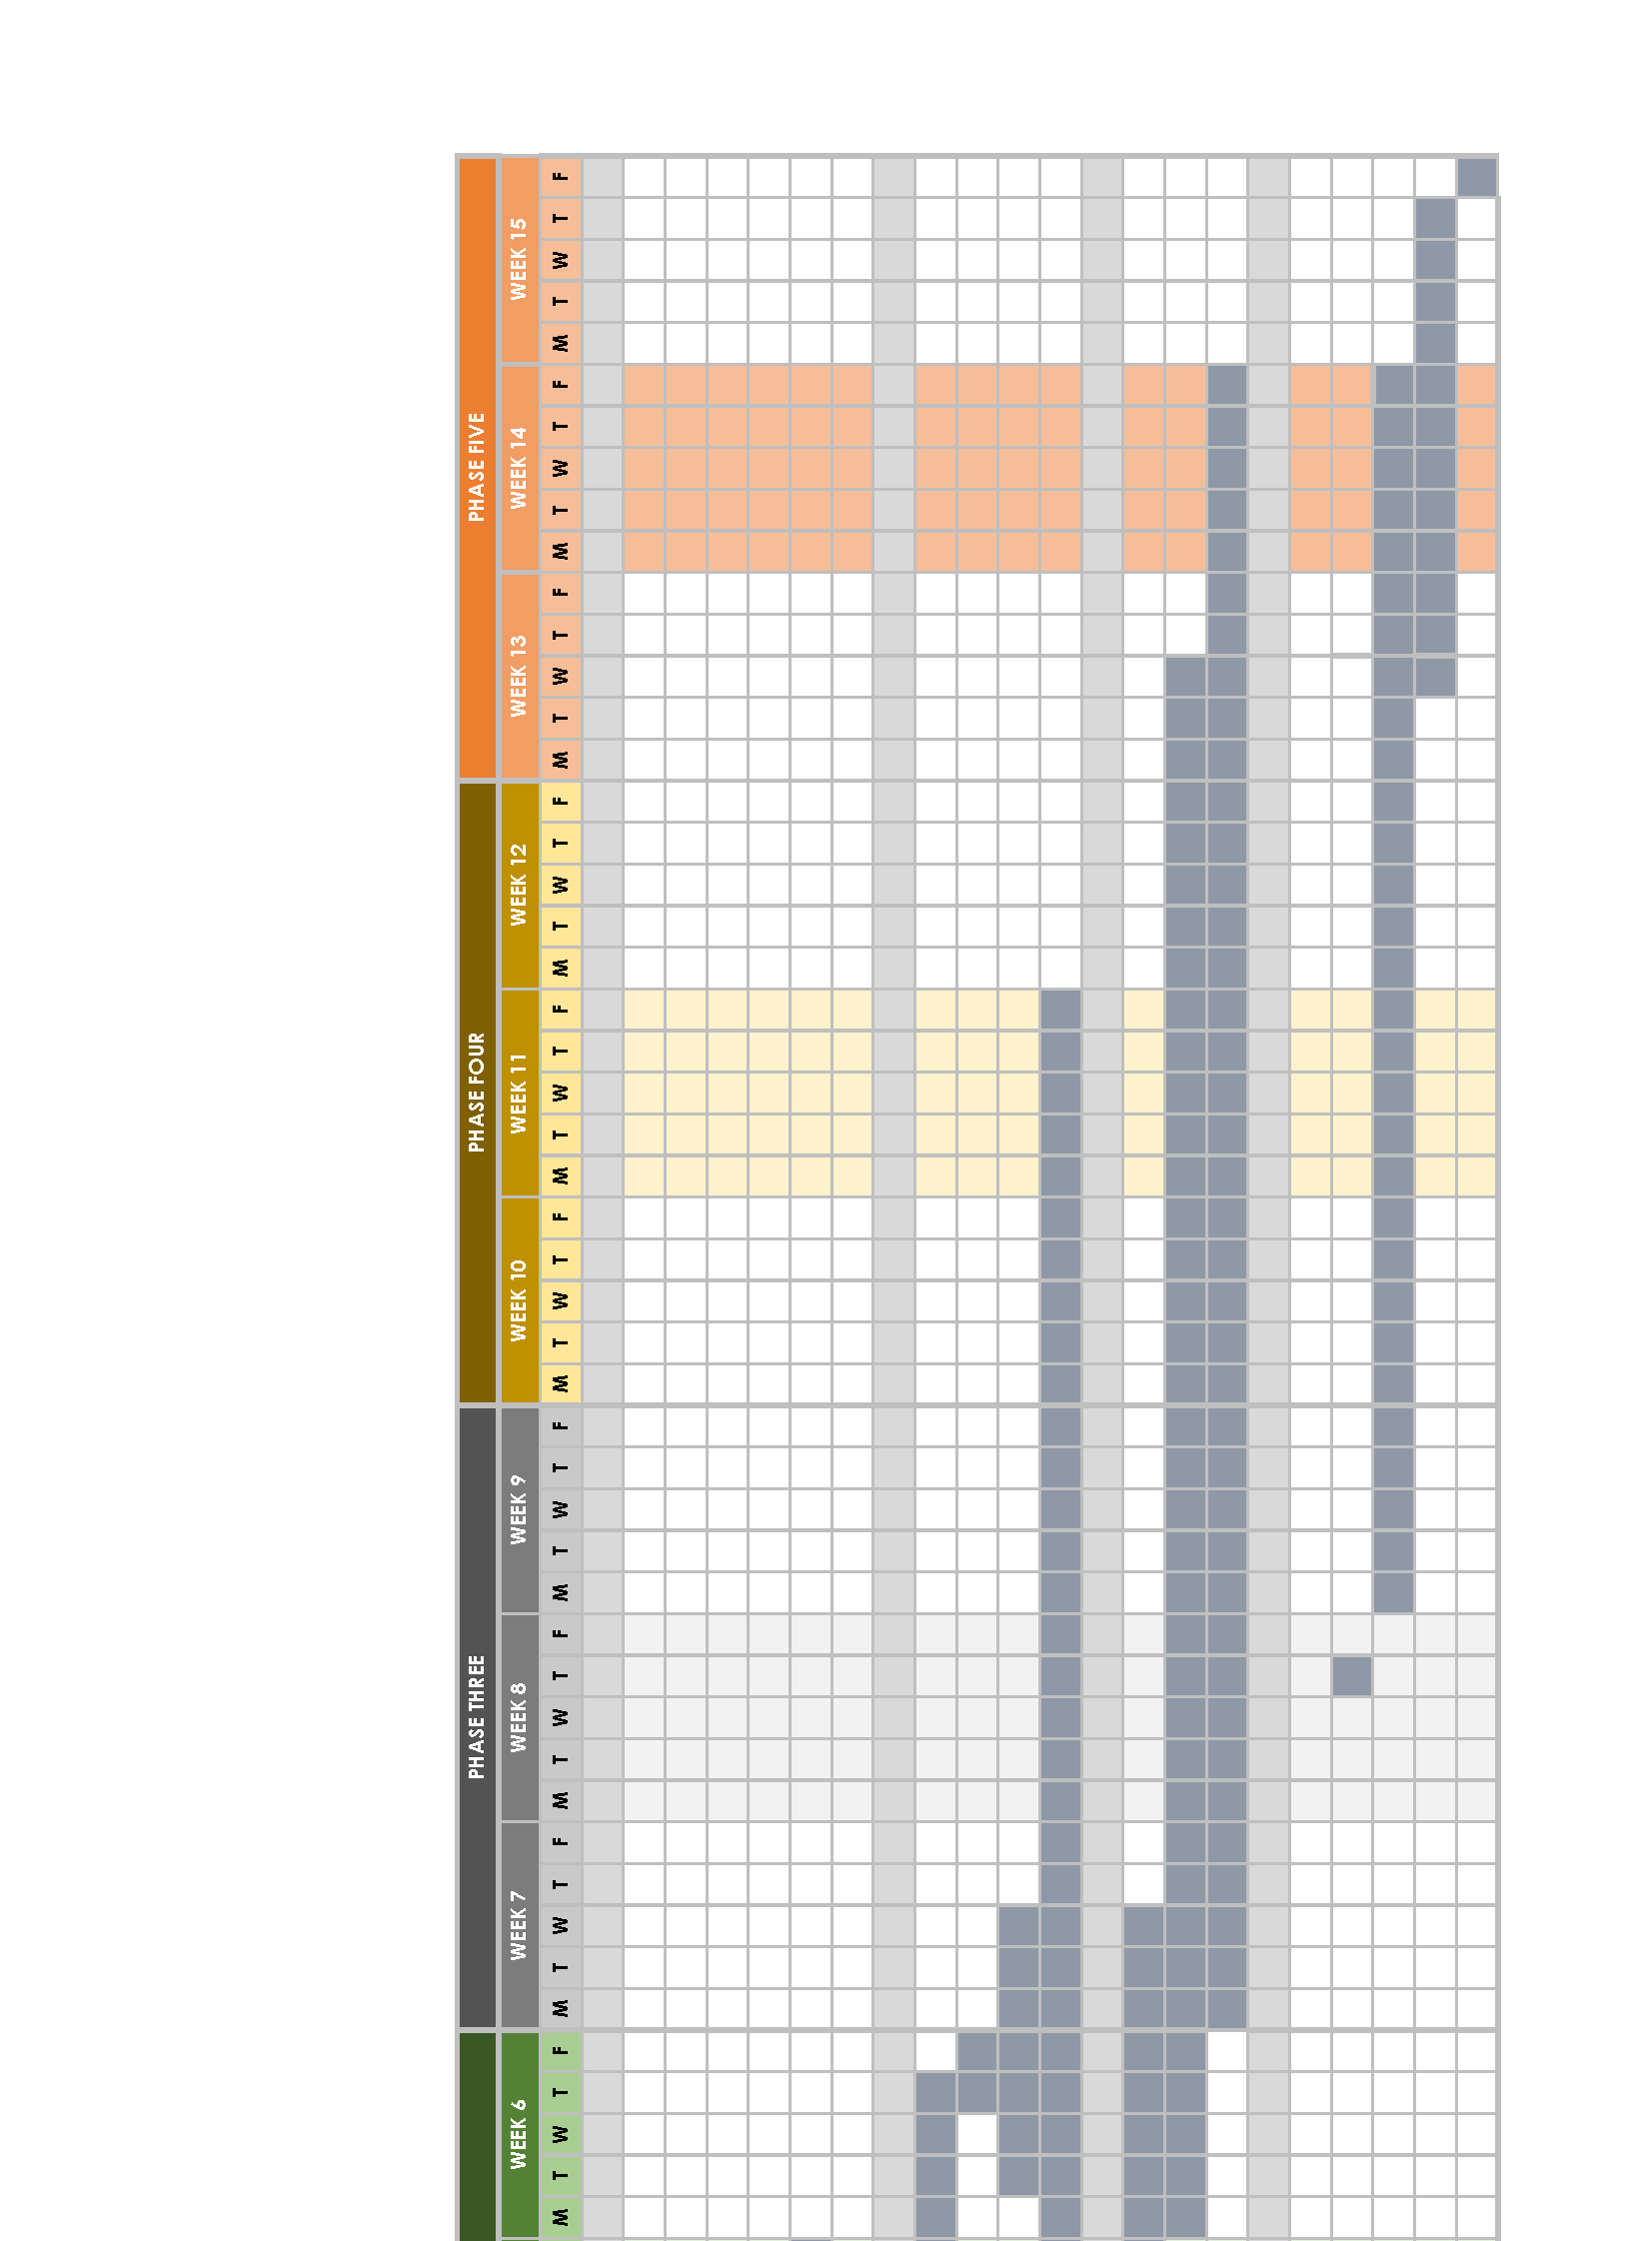
\includepdf[pages=-]{Gantt_BAA.pdf}

\section{Dataset}
\label{sec:Dataset}
Detailed information on image quality assessment (IQA) databases: \par
\begin{itemize}
    \item \textbf{LIVE} (Laboratory for Image \& Video Engineering) dataset \autocite{LIVE} includes 29 reference images and 779 manually distorted images corrupted by 5 types of distortions: JPEG compression (JPEG), JPEG2000 compression (JP2K), white noise (WN), Gaussian blur (GB), and simulated fast fading Rayleigh channel (FF). Each distortion type contains 5 or 4 distortion levels. Most images are 768 $\times$ 512 pixels in size. Each distorted image in this dataset is associated with a Differential Mean Opinion Score (DMOS), scaled from 0 to 100, where 0 indicates no perceivable distortion. 
    \item \textbf{TID2008} (Tampere image database 2008) dataset \autocite{TID2008} includes 25 reference images and 1700 distorted images corrupted by 17 types of distortions, with 4 levels for each distortion type. All images have a fixed resolution of 512 $\times$ 384. This dataset provides MOS values and their standard deviations, with MOS ranging from 0 to 9, where 9 signifies a distortion-free image.
    \item \textbf{TID2013} (Tampere image database 2013) dataset \autocite{TID2013} is extended from TID2008 \autocite{TID2008} by increasing the number of distortion levels to 5, and the number of distortion types to 24. Therefore, 3000 distorted images are generated from 25 pristine images. The subjective testing and data processing steps are similar to that of TID2008. DMOS values for this dataset were derived from over half a million ratings given by nearly a thousand observers, with values ranging from 0 to 9, where higher values denote poorer image quality.
    \item \textbf{CSIQ} (Categorical subjective image quality (CSIQ) database) \autocite{CSIQ} contains 30 pristine images and 866 distorted images corrupted by JPEG, JP2K, WN, GB, additive pink Gaussian noise, and global contrast decrements, with 5 or 4 levels for each distortion type. The resolution is 512 $\times$ 512. Each image in CSIQ is associated with DMOS values obtained from subjective ratings by 25 testers, with DMOS values scaled from 0 to 1, where higher values indicate worse quality.
    \item \textbf{A57} \autocite{A57} includes 3 pristine images and 54 distorted images corrupted by 6 types of distortions, with 3 levels for each distortion type. All images are in gray scale. The resolution is 512 $\times$ 512.
    \item \textbf{WED} (Waterloo exploration database) \autocite{WED} includes 4744 pristine natural images and 94880 distorted images corrupted by JPEG, JP2K, GB, and WN, with 5 levels for each distortion type. The images have various resolutions. No human opinion score is provided, but the authors introduce several alternative test criteria to evaluate the IQA models.
\end{itemize}

\textbf{Multiple Distortions IQA Databases}
\begin{itemize}
    \item \textbf{LIVEMD} (LIVE multiply distorted) \autocite{LIVEMD} database consists of 15 reference images and 405 multiply distorted images. The database includes one/double-fold artifacts. Each multiply distorted image is corrupted under two multiple distortion scenarios: Gaussian blur followed by JPEG and Gaussian blur followed by white noise. All images have a resolution of 1280 $\times$ 720. DMOS values for each distorted image range from 0 to 100.
    \item \textbf{Multiply distorted image database 2013 (MDID2013)} \autocite{MDID2013}: MDID2013 has a total of 12 pristine images and 324 distorted images. Each pristine image is corrupted successively by Gaussian blur, white noise, and JPEG. The images have resolutions of 768 $\times$ 512 or 1280 $\times$ 720.
    \item \textbf{Multiply distorted image database 2016 (MDID2016)} \autocite{MDID2016}: MDID2016 consists of 20 reference images and 1600 distorted images. Five distortion types are introduced, i.e., white noise, Gaussian blur, JPEG, JPEG2000, and contrast change (CC). The order of distortions is as follows: Gaussian blur or CC first, JPEG or JPEG2000 second, and white noise last. All distorted images are with random types and levels of distortions. The image resolution is 512 $\times$ 384.
\end{itemize}

\textbf{Screen Content IQA Databases}
\begin{itemize}
    \item \textbf{Screen Image Quality Assessment Database (SIQAD)} \autocite{SIQAD}: SIQAD includes 20 pristine and 980 distorted screen content images (SCIs). Distortion types include white noise (WN), Gaussian blur (GB), color cast (CC), JPEG, JPEG2000 (JP2K), motion blur (MB), and layer segmentation-based compression, with 7 levels for each type. The images have various resolutions near 700 $\times$ 700.
    \item \textbf{Screen Content Image Quality (SCIQ) Database} \autocite{SCIQ}: SCIQ consists of 40 pristine and 1800 distorted SCIs corrupted by 9 types of distortions, including WN, GB, MB, CC, JPEG, JP2K, color saturation change (CSC), color quantization with dithering (CQD), and the screen content coding extension of High Efficiency Video Coding (HEVC-SCC). Five distortion levels are considered. The resolution is fixed at 1280 $\times$ 720.
    \item \textbf{Cross-Content-Type (CCT) Database} \autocite{CCT}: CCT is constructed to conduct cross-content-type IQA research. CCT consists of 72 pristine and 1320 distorted natural scene images (NSIs), computer graphic images (CGIs), and SCIs. Two distortion types are considered, i.e., HEVC and HEVC-SCC coding, with 11 distortion levels for each type. The image resolution is either 1920 $\times$ 1080 or 1280 $\times$ 720.
    \item \textbf{Hybrid Screen Content and Natural Scene Image Database (HSNID)} \autocite{HSNID}: HSNID has 10 pristine NSIs and 10 pristine SCIs, and 600 distorted NSIs and SCIs corrupted by WN, GB, MB, CC, JPEG, and JP2K, with 5 distortion levels for each type.
\end{itemize}

\textbf{Authentic Distortions IQA Databases}
\begin{itemize}
    \item \textbf{LIVE in the wild image quality challenge database} \autocite{LIVE_Wild} includes 1162 authentically distorted images captured using a variety of mobile devices. Complex real distortions, which are not well-modeled by the synthetic distortions are included. All images are cropped to the resolution of 500 $\times$ 500. A novel crowdsourcing system was employed to gather over 350,000 opinion scores from 8100 observers, ensuring the objectivity of the MOS values obtained.
    \item \textbf{Camera image database (CID2013)} \autocite{CID2013}: CID2013 is designed to test no-reference IQA algorithms. It includes 480 real images captured from 8 typical scenes using 79 consumer cameras and mobile phones. The images are rated from 5 aspects: the overall quality, sharpness, graininess, lightness, and color saturation scales. The images are scaled to a size of 1600 $\times$ 1200.
\end{itemize}

\clearpage
\section{Degradation Types}
\label{sec:Degradation_Types}
The dataset used in this thesis is augmented with synthetic degradations. The following figures below show the different levels of intensity for the degradations of each distortion group. \par
\begin{figure*}[ht]
    \centering
    \setlength{\tabcolsep}{1pt}
    \Large
    \resizebox{\textwidth}{!}{%
        \begin{tabular}{C{5em}ccccc}
            & Level 1 & Level 2 & Level 3 & Level 4 & Level 5 \\
            Brighten & 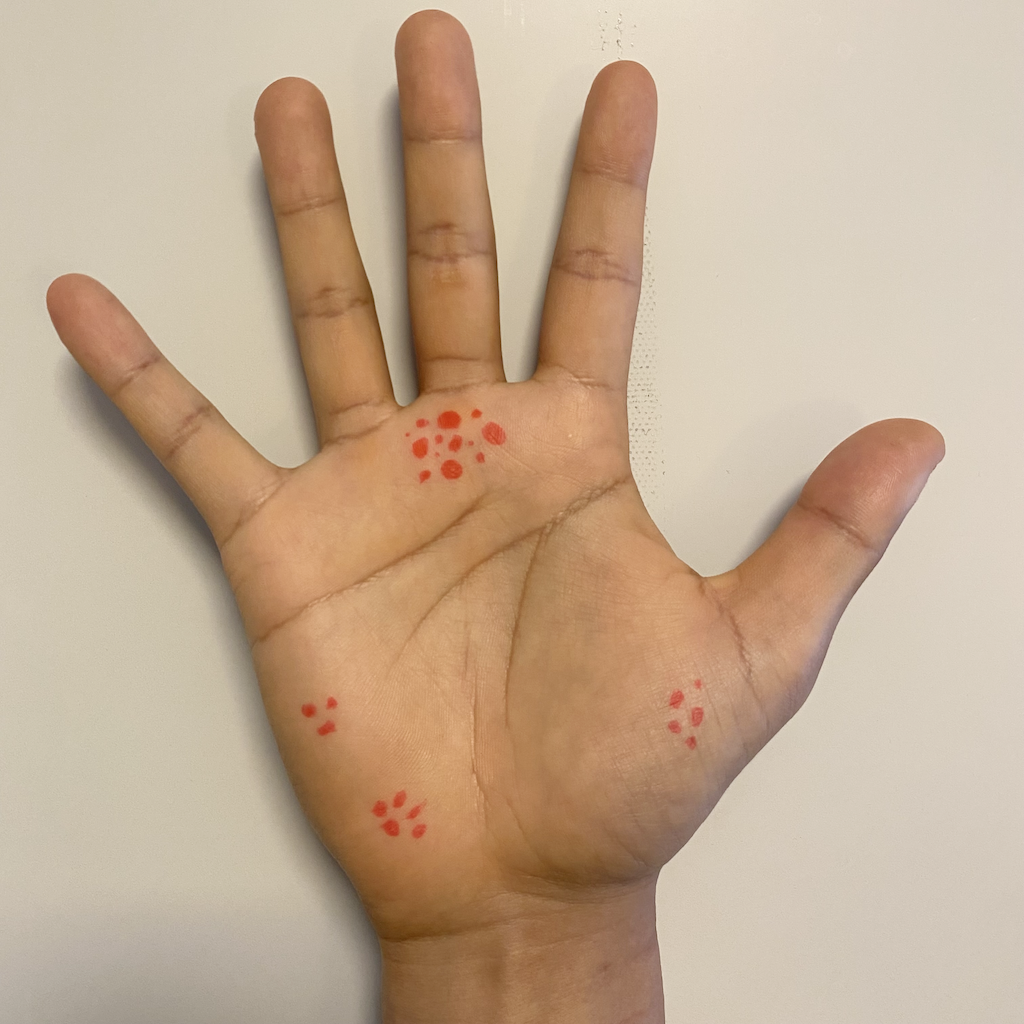
\includegraphics[width=\gridimagewidth,valign=m]{img/supplementary/lighting/brighten/0_brighten_0.0.png} & 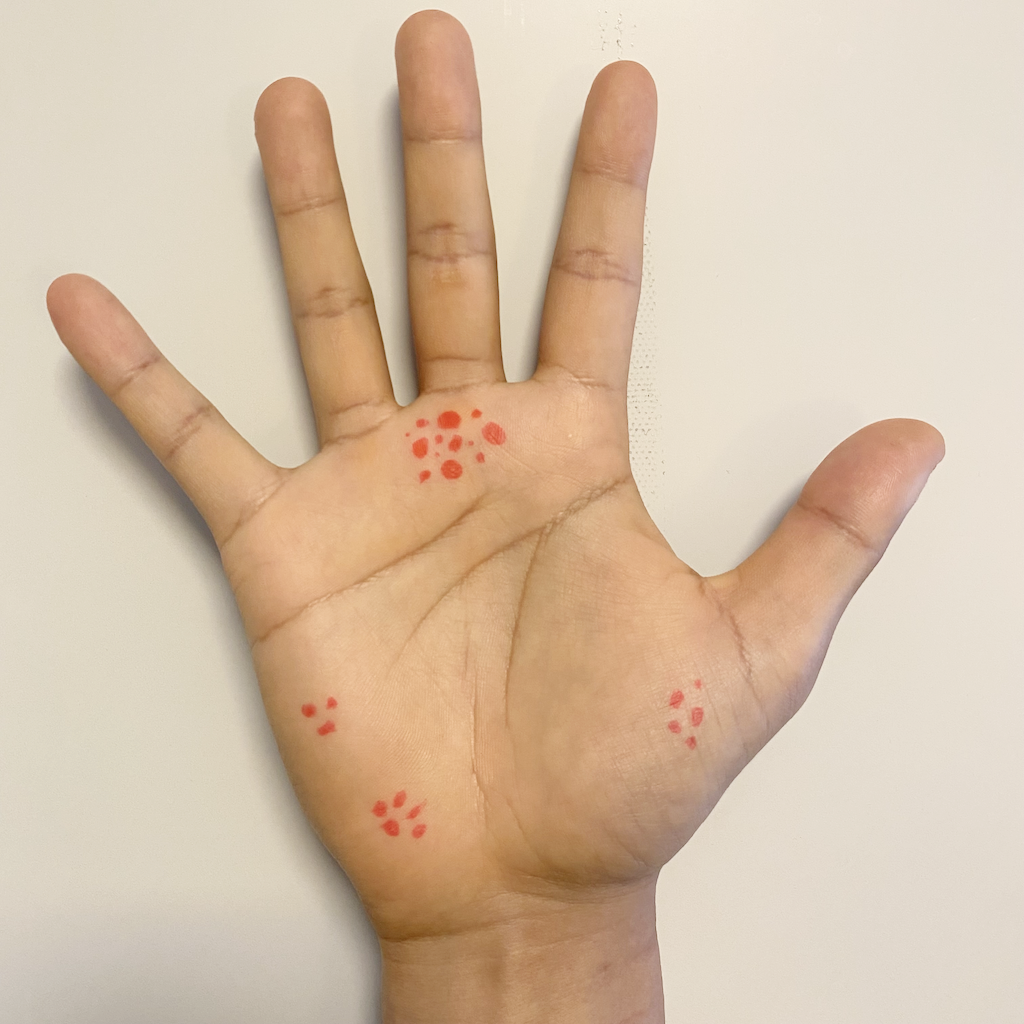
\includegraphics[width=\gridimagewidth,valign=m]{img/supplementary/lighting/brighten/0_brighten_0.2.png} & 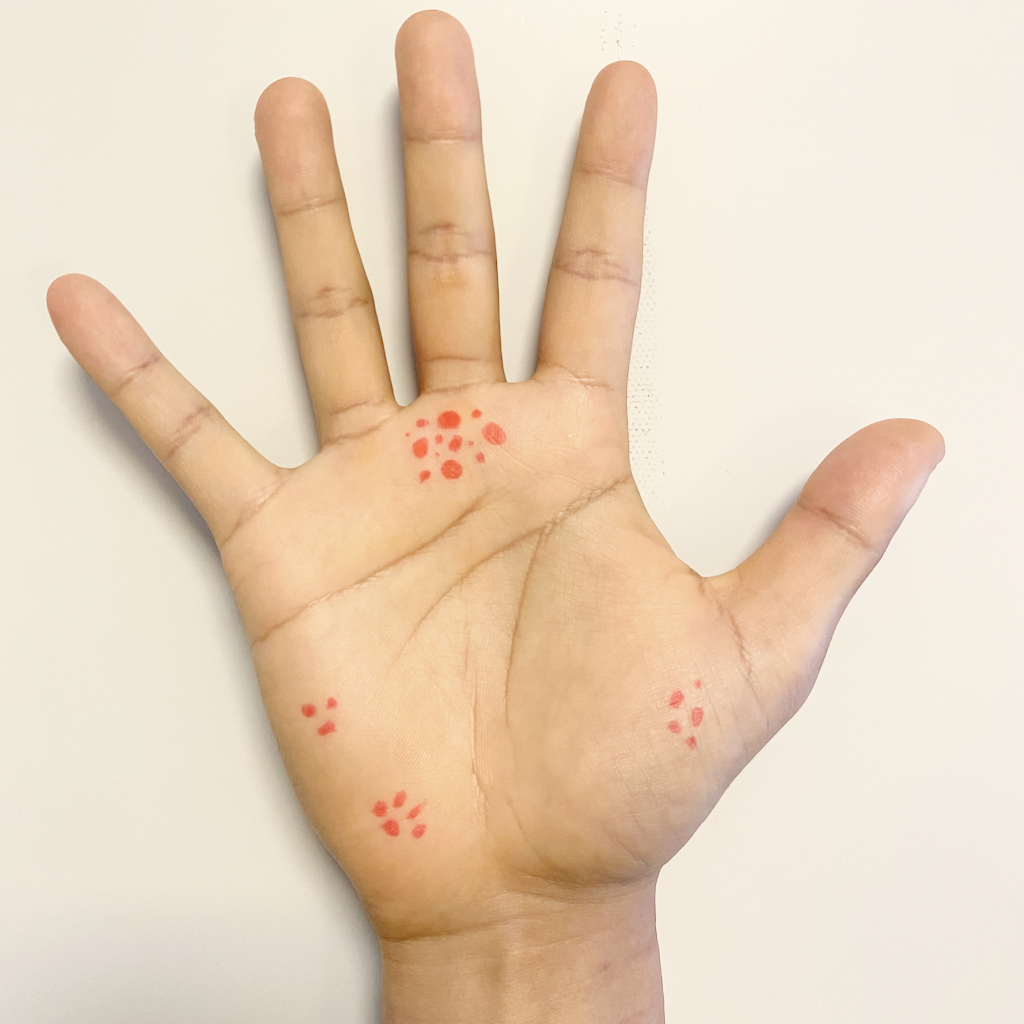
\includegraphics[width=\gridimagewidth,valign=m]{img/supplementary/lighting/brighten/0_brighten_0.4.png} & 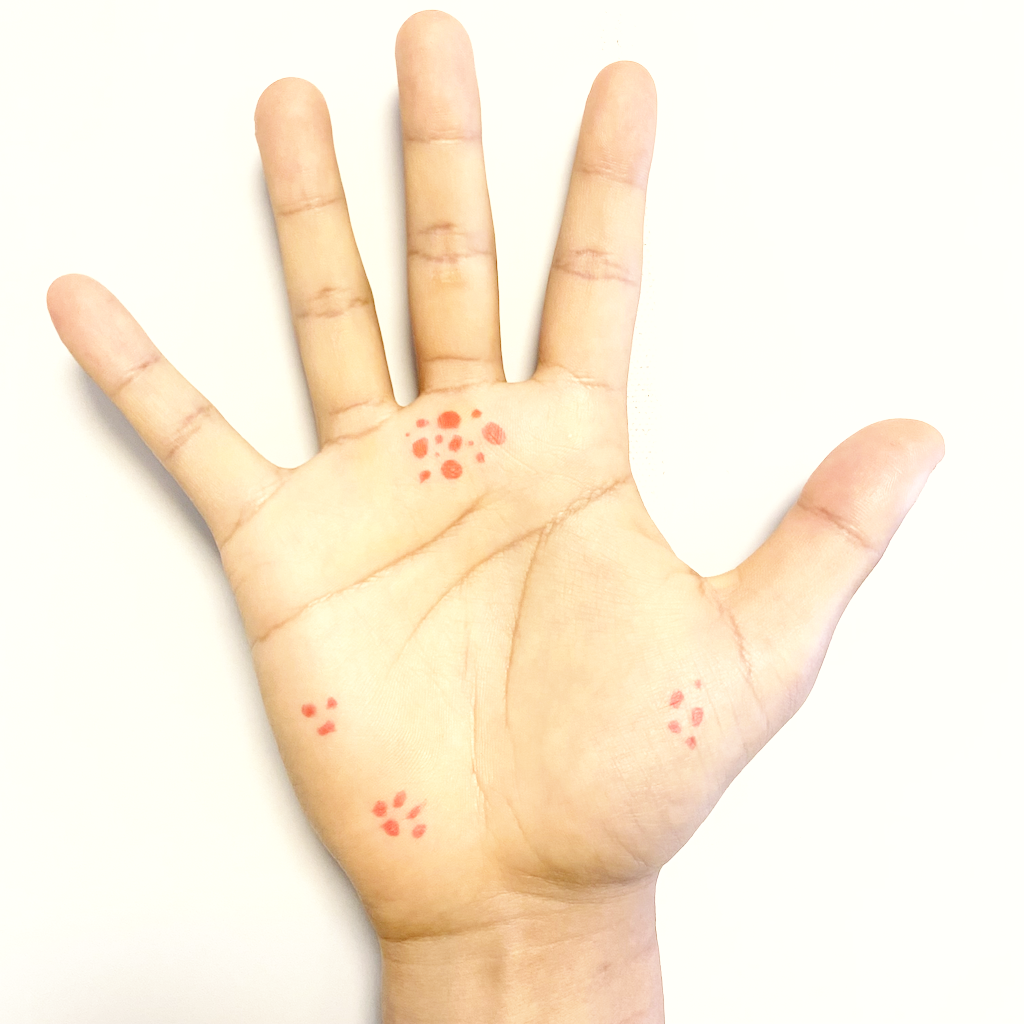
\includegraphics[width=\gridimagewidth,valign=m]{img/supplementary/lighting/brighten/0_brighten_0.7.png} & 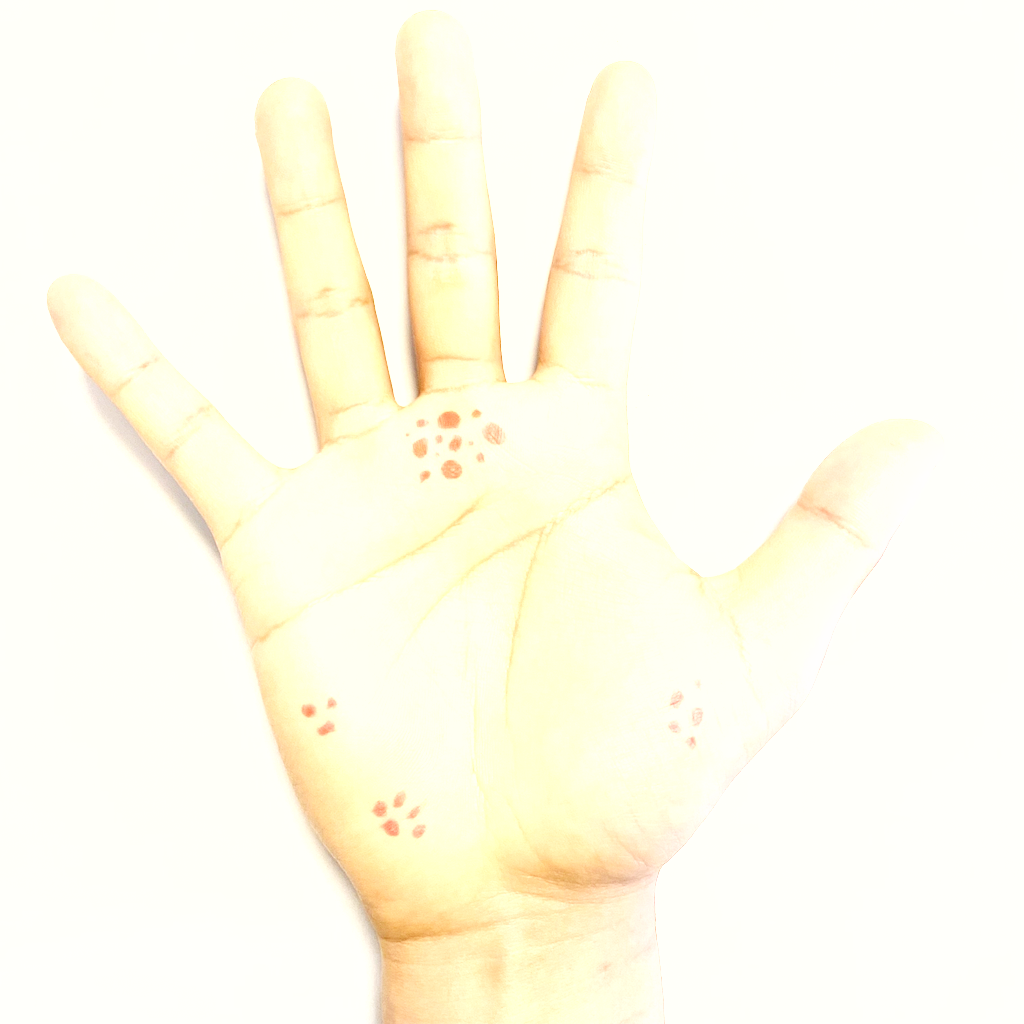
\includegraphics[width=\gridimagewidth,valign=m]{img/supplementary/lighting/brighten/0_brighten_1.1.png} \\ [6.15ex]
            Darken & 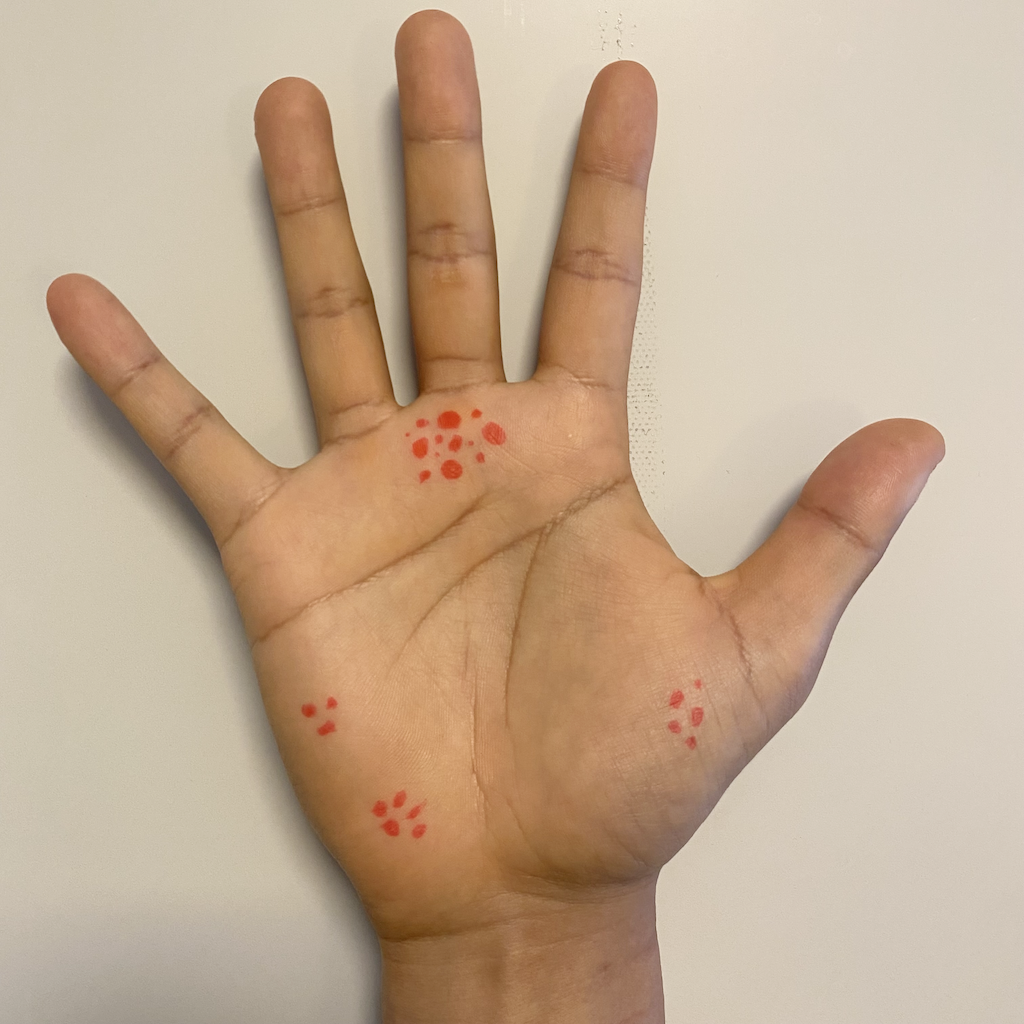
\includegraphics[width=\gridimagewidth,valign=m]{img/supplementary/lighting/darken/0_darken_0.0.png} & 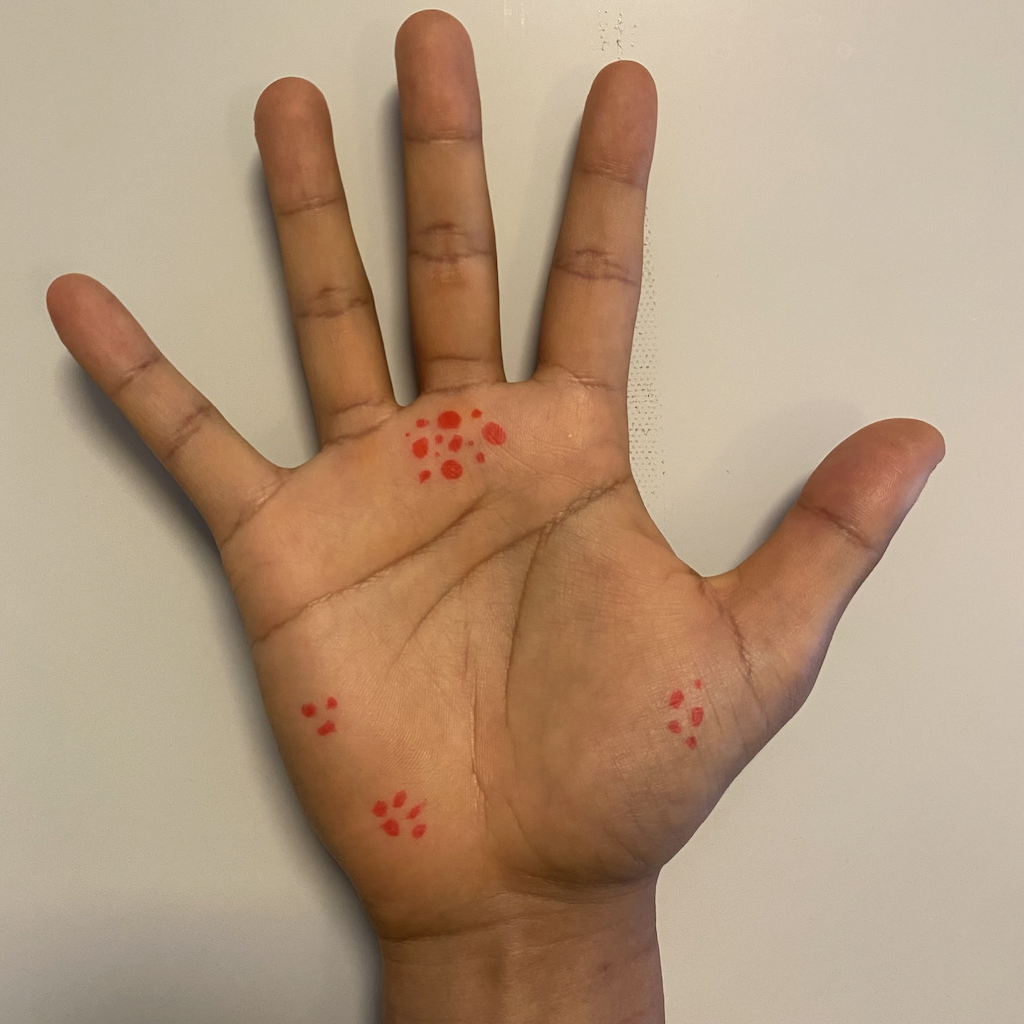
\includegraphics[width=\gridimagewidth,valign=m]{img/supplementary/lighting/darken/0_darken_0.2.png} & 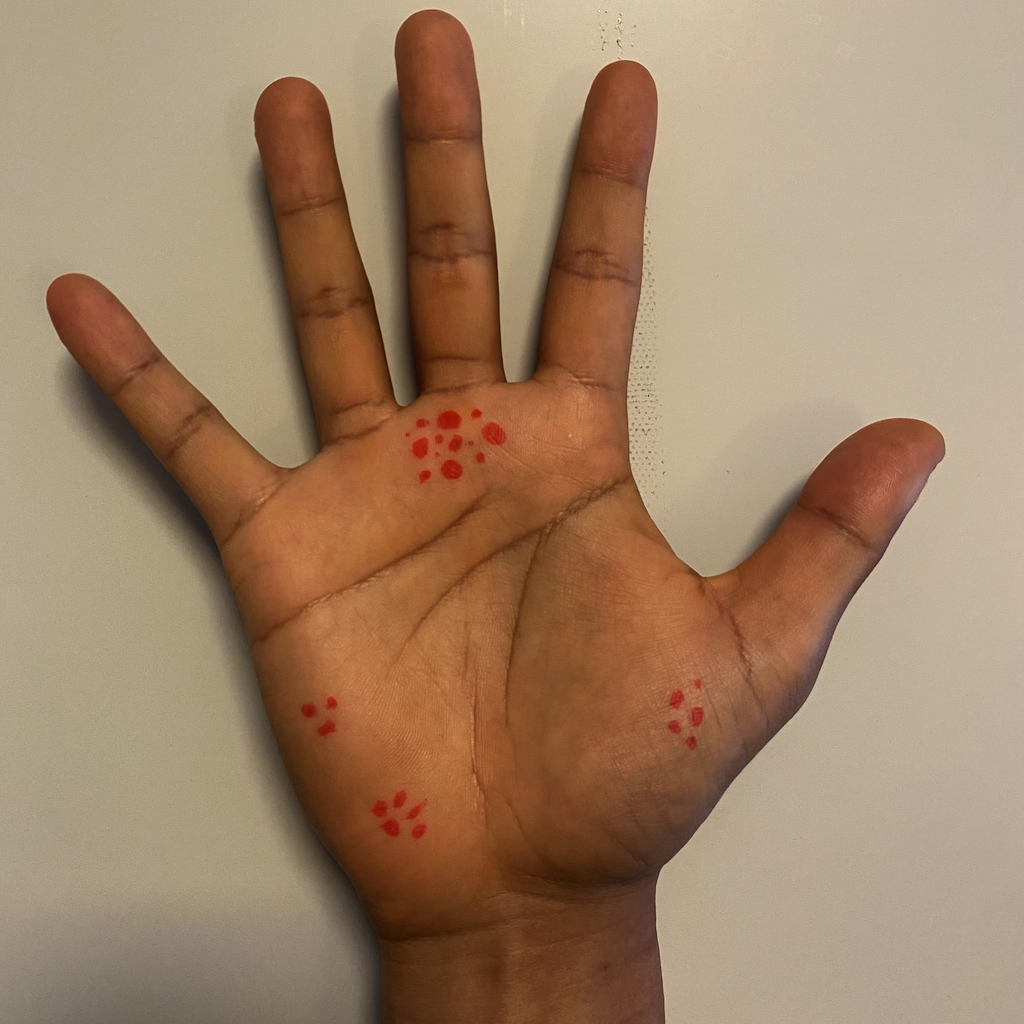
\includegraphics[width=\gridimagewidth,valign=m]{img/supplementary/lighting/darken/0_darken_0.4.png} & 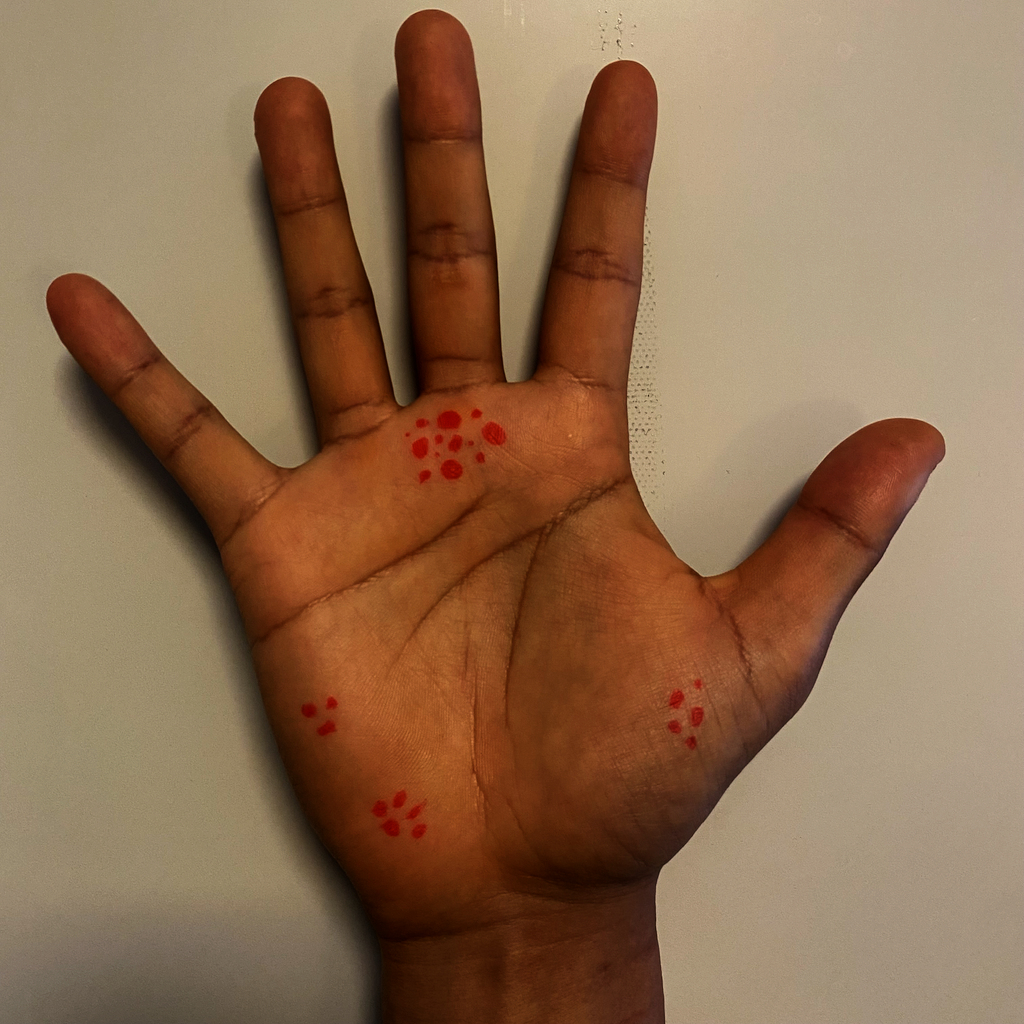
\includegraphics[width=\gridimagewidth,valign=m]{img/supplementary/lighting/darken/0_darken_0.6.png} & 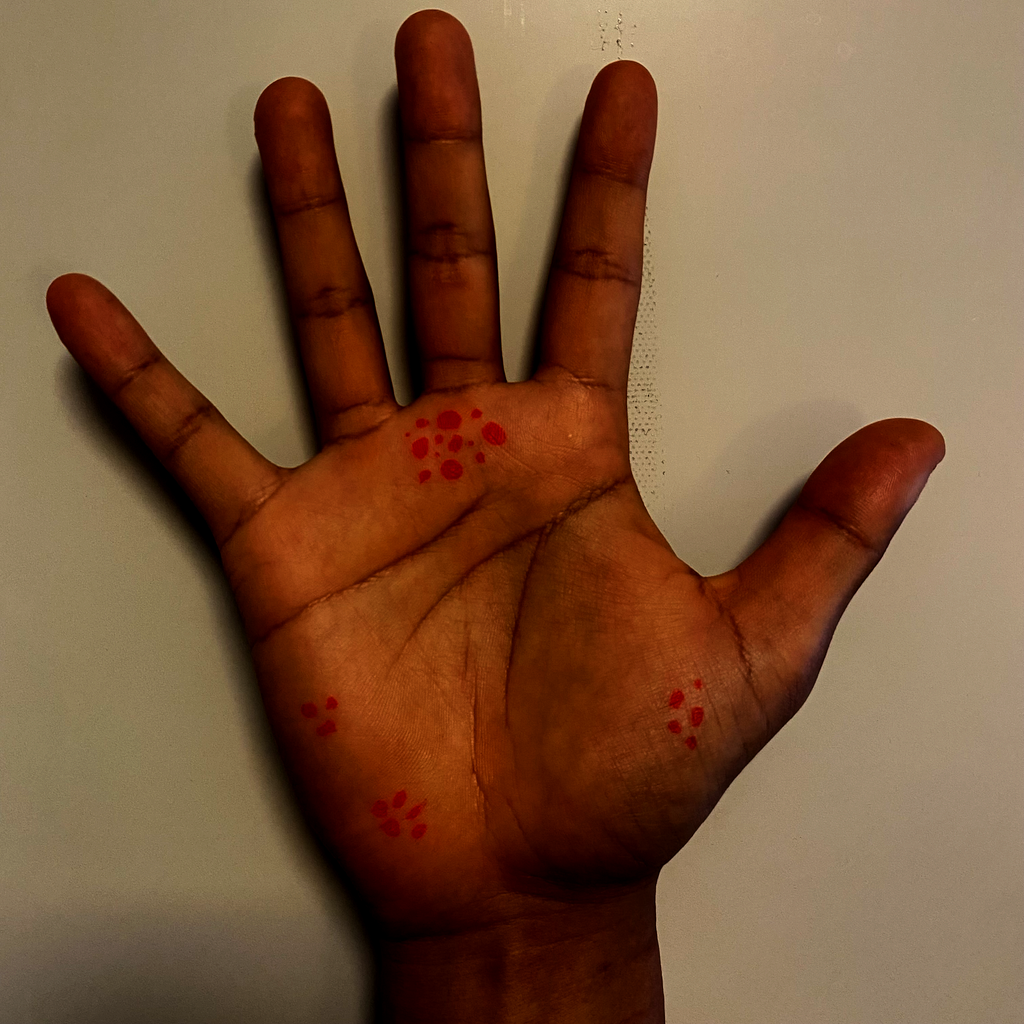
\includegraphics[width=\gridimagewidth,valign=m]{img/supplementary/lighting/darken/0_darken_0.8.png} \\ [6.15ex]
        \end{tabular}
    }
    \caption{Visualization of the degradation types belonging to the \textit{Brightness change} group for increasing levels of intensity.}
    \label{fig:brightness_change_supplementary}
\end{figure*}

\begin{figure*}[ht]
    \centering
    \setlength{\tabcolsep}{1pt}
    \Large
    \resizebox{\textwidth}{!}{%
        \begin{tabular}{C{5em}ccccc}
            & Level 1 & Level 2 & Level 3 & Level 4 & Level 5 \\
            Color block & 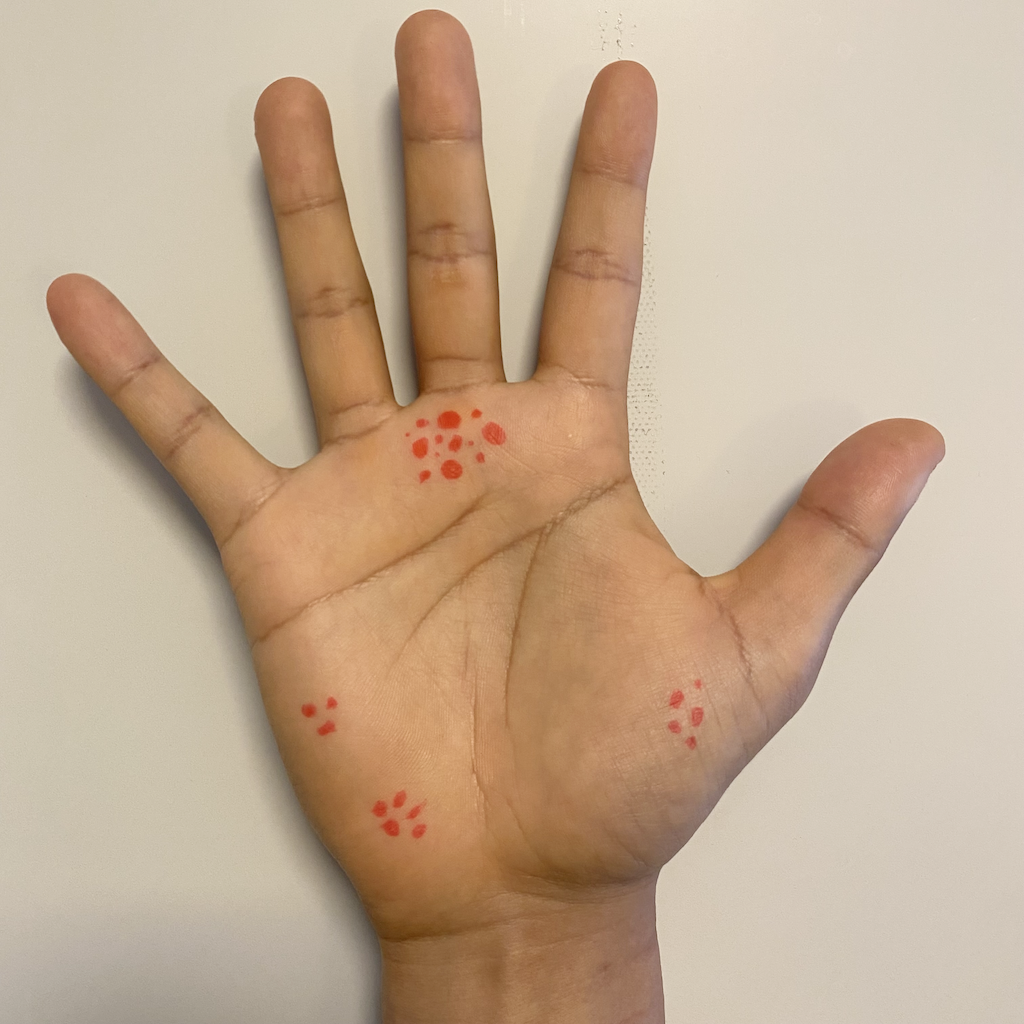
\includegraphics[width=\gridimagewidth,valign=m]{img/supplementary/background/color_block/0_color_block_0.0.png} & 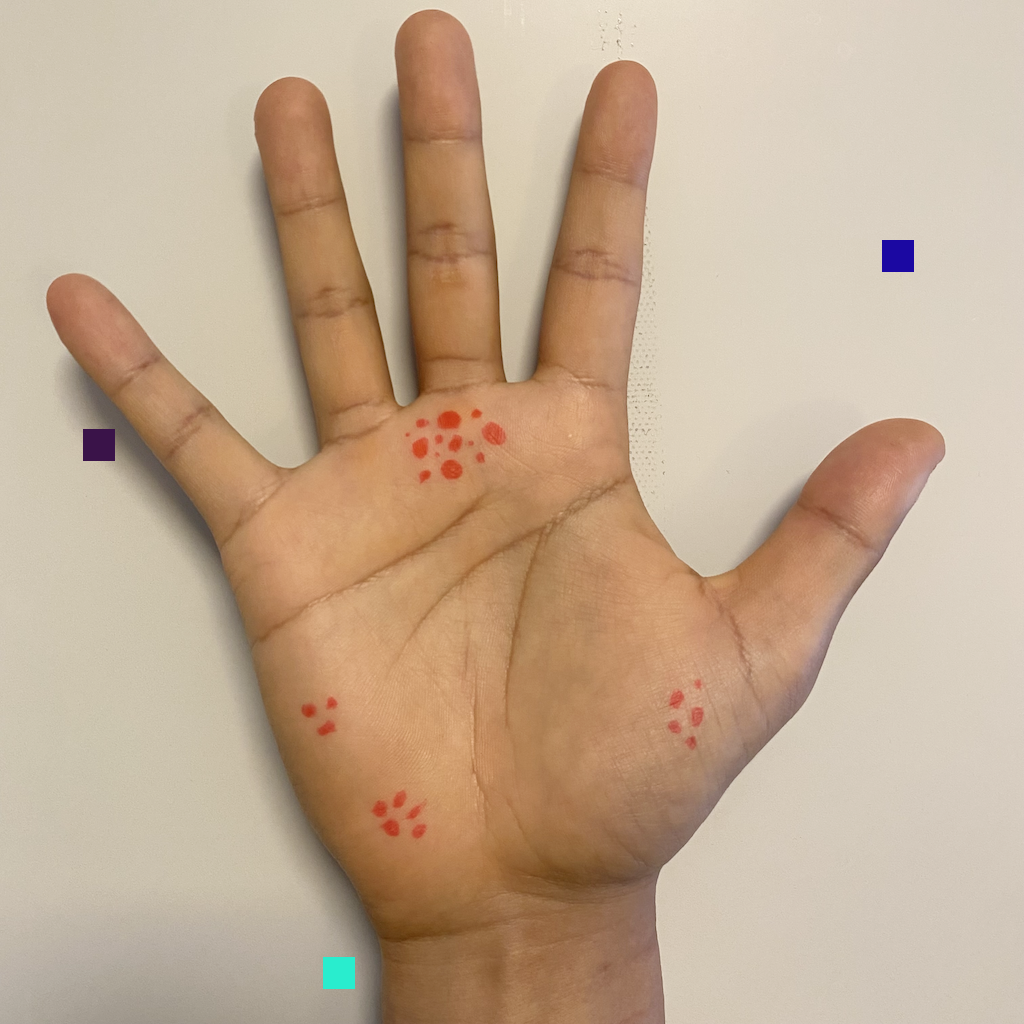
\includegraphics[width=\gridimagewidth,valign=m]{img/supplementary/background/color_block/0_color_block_0.5.png} & 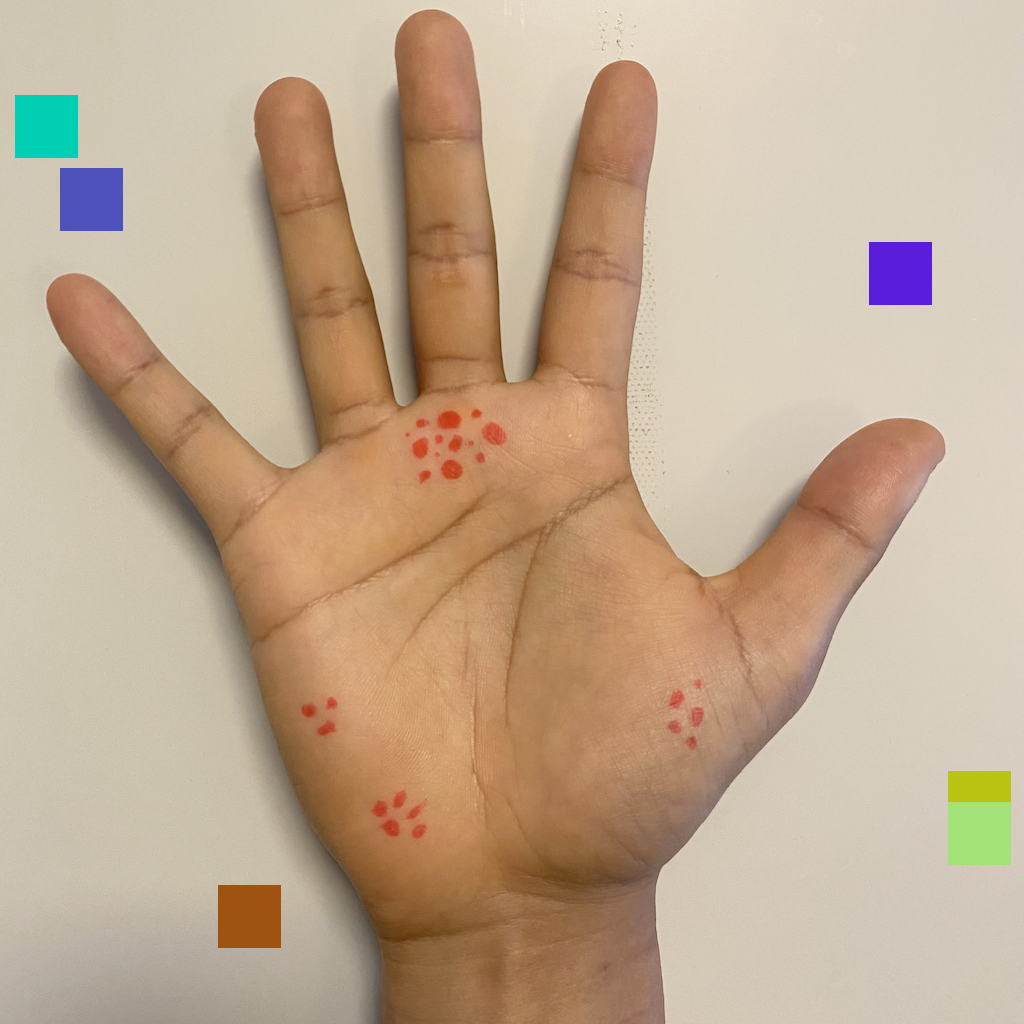
\includegraphics[width=\gridimagewidth,valign=m]{img/supplementary/background/color_block/0_color_block_1.0.png} & 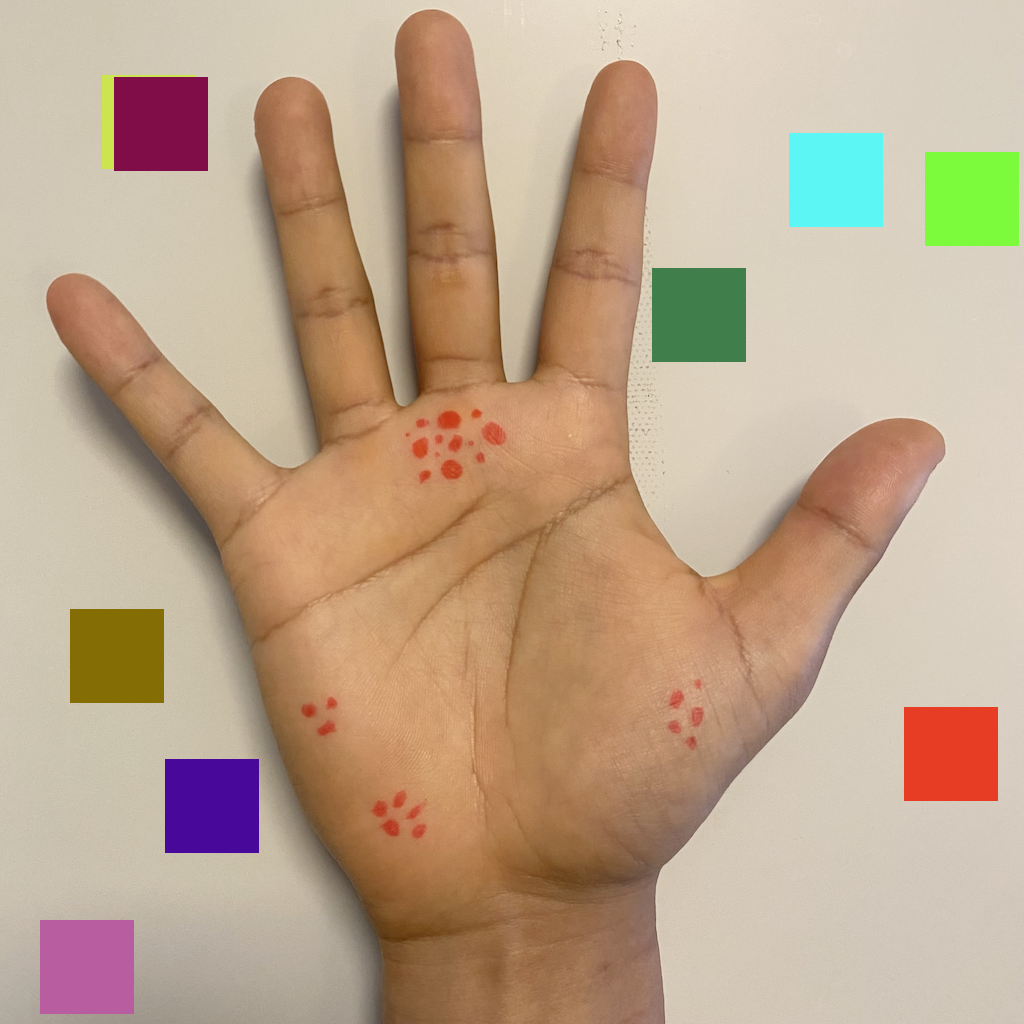
\includegraphics[width=\gridimagewidth,valign=m]{img/supplementary/background/color_block/0_color_block_1.5.png} & 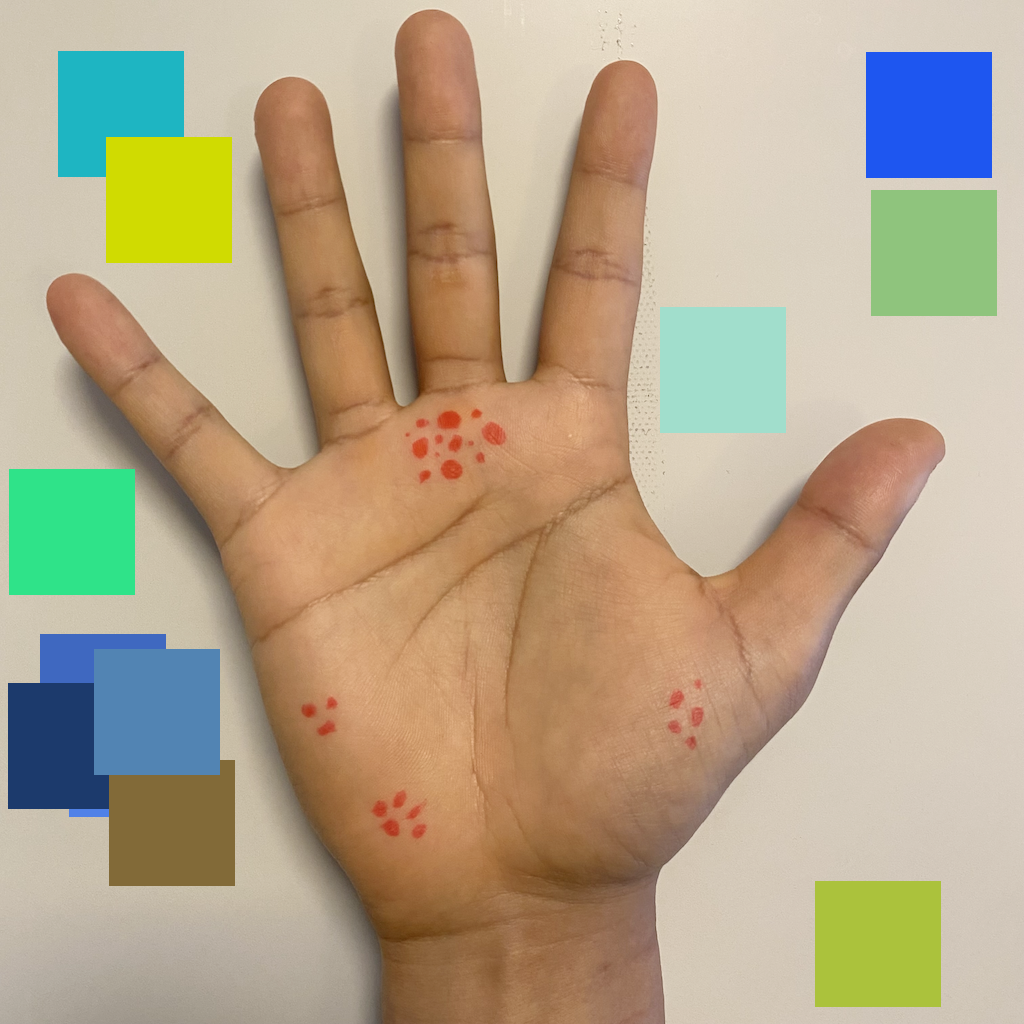
\includegraphics[width=\gridimagewidth,valign=m]{img/supplementary/background/color_block/0_color_block_2.0.png} \\ [6.15ex]
        \end{tabular}
    }
    \caption{Visualization of the degradation types belonging to the \textit{Background color} group for increasing levels of intensity.}
    \label{fig:background_supplementary}
\end{figure*}

\begin{figure*}[ht]
    \centering
    \setlength{\tabcolsep}{1pt}
    \Large
    \resizebox{\textwidth}{!}{%
        \begin{tabular}{C{5em}ccccc}
            & Level 1 & Level 2 & Level 3 & Level 4 & Level 5 \\
            Field of view & 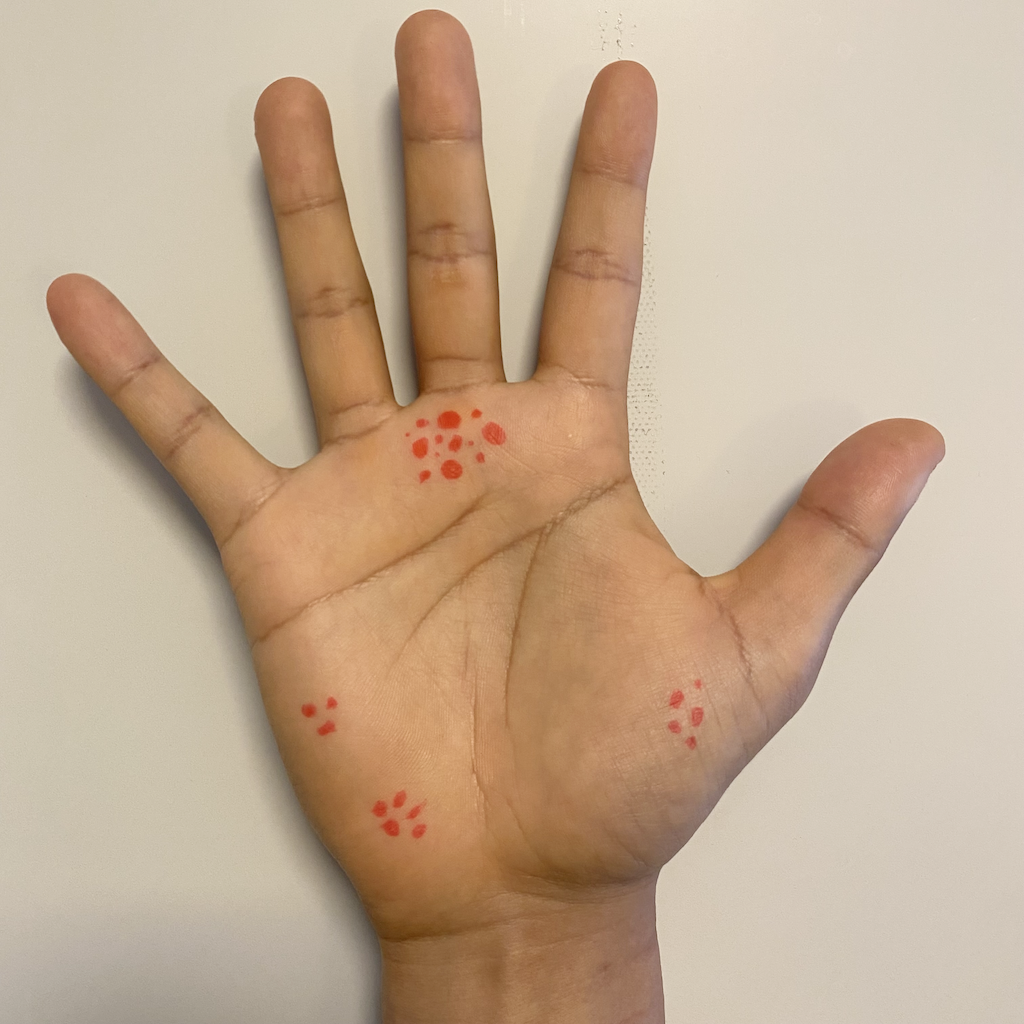
\includegraphics[width=\gridimagewidth,valign=m]{img/supplementary/field_of_view/crop_image/0_crop_image_0.png} & \includegraphics[width=\gridimagewidth,valign=m]{img/supplementary/field_of_view/crop_image/0_crop_image_1.png} & \includegraphics[width=\gridimagewidth,valign=m]{img/supplementary/field_of_view/crop_image/0_crop_image_2.png} & \includegraphics[width=\gridimagewidth,valign=m]{img/supplementary/field_of_view/crop_image/0_crop_image_3.png} & \includegraphics[width=\gridimagewidth,valign=m]{img/supplementary/field_of_view/crop_image/0_crop_image_4.png} \\ [6.15ex]
        \end{tabular}
    }
    \caption{Visualization of the degradation types belonging to the \textit{Field of View} group for increasing levels of intensity.}
    \label{fig:field_of_view_supplementary}
\end{figure*}

\begin{figure*}[ht]
    \centering
    \setlength{\tabcolsep}{1pt}
    \Large
    \resizebox{\textwidth}{!}{%
        \begin{tabular}{C{5em}ccccc}
            & Level 1 & Level 2 & Level 3 & Level 4 & Level 5 \\
            Perspective bottom & \includegraphics[width=\gridimagewidth,valign=m]{img/supplementary/orientation/perspective_bottom/0_perspective_bottom_0.0.png} & \includegraphics[width=\gridimagewidth,valign=m]{img/supplementary/orientation/perspective_bottom/0_perspective_bottom_0.2.png} & \includegraphics[width=\gridimagewidth,valign=m]{img/supplementary/orientation/perspective_bottom/0_perspective_bottom_0.4.png} & \includegraphics[width=\gridimagewidth,valign=m]{img/supplementary/orientation/perspective_bottom/0_perspective_bottom_0.6.png} & \includegraphics[width=\gridimagewidth,valign=m]{img/supplementary/orientation/perspective_bottom/0_perspective_bottom_0.8.png} \\ [6.15ex]
            Perspective top & \includegraphics[width=\gridimagewidth,valign=m]{img/supplementary/orientation/perspective_top/0_perspective_top_0.0.png} & \includegraphics[width=\gridimagewidth,valign=m]{img/supplementary/orientation/perspective_top/0_perspective_top_0.2.png} & \includegraphics[width=\gridimagewidth,valign=m]{img/supplementary/orientation/perspective_top/0_perspective_top_0.4.png} & \includegraphics[width=\gridimagewidth,valign=m]{img/supplementary/orientation/perspective_top/0_perspective_top_0.6.png} & \includegraphics[width=\gridimagewidth,valign=m]{img/supplementary/orientation/perspective_top/0_perspective_top_0.8.png} \\ [6.15ex]
            Perspective left & \includegraphics[width=\gridimagewidth,valign=m]{img/supplementary/orientation/perspective_left/0_perspective_left_0.0.png} & \includegraphics[width=\gridimagewidth,valign=m]{img/supplementary/orientation/perspective_left/0_perspective_left_0.2.png} & \includegraphics[width=\gridimagewidth,valign=m]{img/supplementary/orientation/perspective_left/0_perspective_left_0.4.png} & \includegraphics[width=\gridimagewidth,valign=m]{img/supplementary/orientation/perspective_left/0_perspective_left_0.6.png} & \includegraphics[width=\gridimagewidth,valign=m]{img/supplementary/orientation/perspective_left/0_perspective_left_0.8.png} \\ [6.15ex]
            Perspective right & \includegraphics[width=\gridimagewidth,valign=m]{img/supplementary/orientation/perspective_right/0_perspective_right_0.0.png} & \includegraphics[width=\gridimagewidth,valign=m]{img/supplementary/orientation/perspective_right/0_perspective_right_0.2.png} & \includegraphics[width=\gridimagewidth,valign=m]{img/supplementary/orientation/perspective_right/0_perspective_right_0.4.png} & \includegraphics[width=\gridimagewidth,valign=m]{img/supplementary/orientation/perspective_right/0_perspective_right_0.6.png} & \includegraphics[width=\gridimagewidth,valign=m]{img/supplementary/orientation/perspective_right/0_perspective_right_0.8.png} \\ [6.15ex]
        \end{tabular}
    }
    \caption{Visualization of the degradation types belonging to the \textit{Image orientation} group for increasing levels of intensity.}
    \label{fig:orientation_supplementary}
\end{figure*}

\begin{figure*}[ht]
    \centering
    \setlength{\tabcolsep}{1pt}
    \Large
    \resizebox{\textwidth}{!}{%
        \begin{tabular}{C{5em}ccccc}
            & Level 1 & Level 2 & Level 3 & Level 4 & Level 5 \\
            Gaussian blur & \includegraphics[width=\gridimagewidth,valign=m]{img/supplementary/focus/gaussian_blur/0_gaussian_blur_0.png} & \includegraphics[width=\gridimagewidth,valign=m]{img/supplementary/focus/gaussian_blur/0_gaussian_blur_1.png} & \includegraphics[width=\gridimagewidth,valign=m]{img/supplementary/focus/gaussian_blur/0_gaussian_blur_2.png} & \includegraphics[width=\gridimagewidth,valign=m]{img/supplementary/focus/gaussian_blur/0_gaussian_blur_3.png} & \includegraphics[width=\gridimagewidth,valign=m]{img/supplementary/focus/gaussian_blur/0_gaussian_blur_5.png} \\ [6.15ex]
            Lens blur & \includegraphics[width=\gridimagewidth,valign=m]{img/supplementary/focus/lens_blur/0_lens_blur_0.png} & \includegraphics[width=\gridimagewidth,valign=m]{img/supplementary/focus/lens_blur/0_lens_blur_2.png} & \includegraphics[width=\gridimagewidth,valign=m]{img/supplementary/focus/lens_blur/0_lens_blur_4.png} & \includegraphics[width=\gridimagewidth,valign=m]{img/supplementary/focus/lens_blur/0_lens_blur_6.png} & \includegraphics[width=\gridimagewidth,valign=m]{img/supplementary/focus/lens_blur/0_lens_blur_8.png} \\ [6.15ex]
            Motion blur & \includegraphics[width=\gridimagewidth,valign=m]{img/supplementary/focus/motion_blur/0_motion_blur_0.png} & \includegraphics[width=\gridimagewidth,valign=m]{img/supplementary/focus/motion_blur/0_motion_blur_2.png} & \includegraphics[width=\gridimagewidth,valign=m]{img/supplementary/focus/motion_blur/0_motion_blur_4.png} & \includegraphics[width=\gridimagewidth,valign=m]{img/supplementary/focus/motion_blur/0_motion_blur_6.png} & \includegraphics[width=\gridimagewidth,valign=m]{img/supplementary/focus/motion_blur/0_motion_blur_8.png} \\ [6.15ex]
        \end{tabular}
    }
    \caption{Visualization of the degradation types belonging to the \textit{Focus} group for increasing levels of intensity.}
    \label{fig:focus_supplementary}
\end{figure*}

\begin{figure*}[ht]
    \centering
    \setlength{\tabcolsep}{1pt}
    \Large
    \resizebox{\textwidth}{!}{%
        \begin{tabular}{C{5em}ccccc}
            & Level 1 & Level 2 & Level 3 & Level 4 & Level 5 \\
            Change resolution & \includegraphics[width=\gridimagewidth,valign=m]{img/supplementary/resolution/change_resolution/0_change_resolution_0.0.png} & \includegraphics[width=\gridimagewidth,valign=m]{img/supplementary/resolution/change_resolution/0_change_resolution_0.2.png} & \includegraphics[width=\gridimagewidth,valign=m]{img/supplementary/resolution/change_resolution/0_change_resolution_0.4.png} & \includegraphics[width=\gridimagewidth,valign=m]{img/supplementary/resolution/change_resolution/0_change_resolution_0.6.png} & \includegraphics[width=\gridimagewidth,valign=m]{img/supplementary/resolution/change_resolution/0_change_resolution_0.8.png} \\ [6.15ex]
        \end{tabular}
    }
    \caption{Visualization of the degradation types belonging to the \textit{Resolution} group for increasing levels of intensity.}
    \label{fig:resolution_supplementary}
\end{figure*}

\begin{figure*}[ht]
    \centering
    \setlength{\tabcolsep}{1pt}
    \Large
    \resizebox{\textwidth}{!}{%
        \begin{tabular}{C{5em}ccccc}
            & Level 1 & Level 2 & Level 3 & Level 4 & Level 5 \\
            Color saturation 1 & \includegraphics[width=\gridimagewidth,valign=m]{img/supplementary/color_calibration/color_saturation1/0_color_saturation1_0.png} & \includegraphics[width=\gridimagewidth,valign=m]{img/supplementary/color_calibration/color_saturation1/0_color_saturation1_0.2.png} & \includegraphics[width=\gridimagewidth,valign=m]{img/supplementary/color_calibration/color_saturation1/0_color_saturation1_0.4.png} & \includegraphics[width=\gridimagewidth,valign=m]{img/supplementary/color_calibration/color_saturation1/0_color_saturation1_0.6.png} & \includegraphics[width=\gridimagewidth,valign=m]{img/supplementary/color_calibration/color_saturation1/0_color_saturation1_0.8.png} \\ [6.15ex]
            Color saturation 2 & \includegraphics[width=\gridimagewidth,valign=m]{img/supplementary/color_calibration/color_saturation2/0_color_saturation2_0.png} & \includegraphics[width=\gridimagewidth,valign=m]{img/supplementary/color_calibration/color_saturation2/0_color_saturation2_1.png} & \includegraphics[width=\gridimagewidth,valign=m]{img/supplementary/color_calibration/color_saturation2/0_color_saturation2_2.png} & \includegraphics[width=\gridimagewidth,valign=m]{img/supplementary/color_calibration/color_saturation2/0_color_saturation2_3.png} & \includegraphics[width=\gridimagewidth,valign=m]{img/supplementary/color_calibration/color_saturation2/0_color_saturation2_4.png} \\ [6.15ex]
        \end{tabular}
    }
    \caption{Visualization of the degradation types belonging to the \textit{Color calibration} group for increasing levels of intensity.}
    \label{fig:color_calibration_supplementary}
\end{figure*}


\clearpage
\section{Proposed Framework for Automated Image Quality Assessment in Teledermatology}
\label{sec:framework}
\begin{figure}[ht]
    \centering
    \includegraphics[keepaspectratio,width=5.2cm]{img/Architecture.png}
    \caption{Overview of the proposed framework for automated image quality assessment in teledermatology. It starts with good quality input images, which go through a distortion pipeline covering seven dermatology quality criteria. The ARNIQA backbone extracts features, and a multi-output regressor predicts the seven quality criteria. The final predictions are visualized with radar charts.}
    \label{fig:Architecture}
\end{figure}



\end{document}